\chapter{Novel targets}\label{chap:16}
Dark matter must carry at least \SI{0.333}{MeV} to lift an electron across the gap of silicon (\cref{sec:1.3}), and the bulk crystals of \cref{chap:10,chap:11,chap:12,chap:13,chap:14,chap:15} extend the reach downward through phonons, magnons and the pair-breaking edge of a superconductor. Other solids have been proposed for channels that these crystals lack, often with projected reaches that a complete treatment moves by orders of magnitude. The slow linear bands of a Dirac material bring the threshold mass of an electronic excitation below \SI{10}{keV} (\cref{sec:7.3}). The published reaches, however, leave the remote bands out of the screening of the dark-matter field, and for ZrTe$_5$ they are too strong by a factor of several thousand. Other targets are limited by their inputs. The dark-photon rate on a glass is its measured loss tangent, which changes seventeenfold between preparations, and a color center counts only if a recoil leaves a defect that a readout finds, but no measurement has isolated the yield of readable defects per recoil. In most cases, then, the limit is a material input and not the framework of \cref{chap:8}: a background dielectric constant, a density of tunneling states, the yield of a defect. The tunneling defects of glasses also release heat at millikelvin temperatures, and their kinetics shape the delayed signals of \cref{sec:19.6} (\cref{fig:16-map}).

\begin{figure}[tbp]
  \centering
  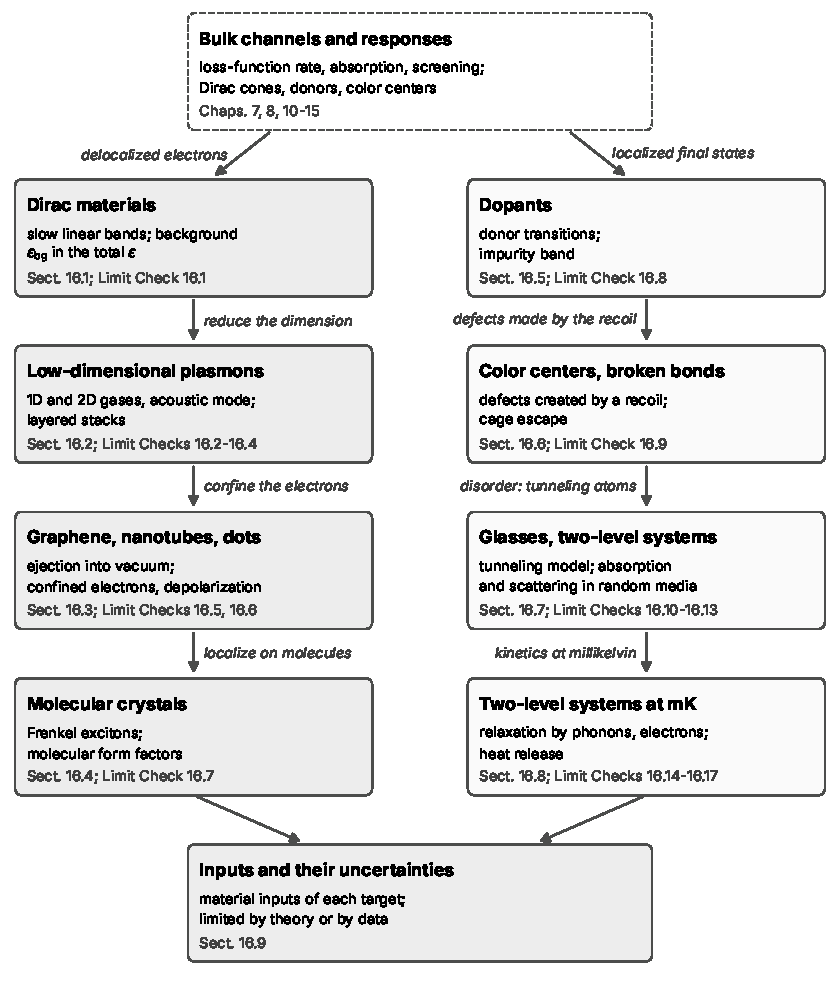
\includegraphics[width=0.85\linewidth]{figures/ch16/map16.pdf}
  \caption{Novel targets, from the bulk responses and rates of \cref{chap:7,chap:8} and \cref{chap:10,chap:11,chap:12,chap:13,chap:14,chap:15}. Left, delocalized electrons: Dirac materials with the background dielectric constant in the total $\varepsilon$ (\cref{sec:16.1}; \cref{lim:16.1a}); electron gases in one and two dimensions and layered stacks (\cref{sec:16.2}; \cref{lim:16.2a,lim:16.2b,lim:16.2c}); graphene, nanotubes and quantum dots (\cref{sec:16.3}; \cref{lim:16.3a,lim:16.3b}); molecular crystals and their Frenkel excitons (\cref{sec:16.4}; \cref{lim:16.4a}). Right, localized final states: dopants (\cref{sec:16.5}; \cref{lim:16.5a}), color centers and broken bonds (\cref{sec:16.6}; \cref{lim:16.6a}), the tunneling two-level systems of glasses and random media (\cref{sec:16.7}; \cref{lim:16.7a,lim:16.7b,lim:16.7c,lim:16.7d}) and their kinetics at millikelvin temperatures (\cref{sec:16.8}; \cref{lim:16.8a,lim:16.8b,lim:16.8c,lim:16.8d}). Both columns feed the table of material inputs and their uncertainties (\cref{sec:16.9}).}
  \label{fig:16-map}
\end{figure}

\section{Dirac-material rates}\label{sec:16.1}

In ZrTe$_5$ the remote bands alone have a dielectric constant of about 50, and the Dirac electrons raise it by \SI{9}{\percent}, to 55 (\cref{we:7-zrte5}). A dark photon that couples to an electron--hole pair in the cone reaches it through both: the field is screened by $|\varepsilon|^2 \approx 3000$, not by the factor $|1 + \varepsilon_{\mathrm{D}}/\varepsilon_{\mathrm{bg}}|^2 = 1.09^2 = 1.2$ that the Dirac electrons contribute alone. The projected reaches of Dirac materials were computed with the second factor~\cite{hochberg2018detection,geilhufe2020dirac}, and for ZrTe$_5$ the two differ by a factor 5200 to 6400 in the scattering rate (\cref{sec:16.1-zrte5}).

\subsection{Loss function of a Dirac target}\label{sec:16.1-loss}

The longitudinal dielectric function is $\varepsilon = 1 - v_{\mathrm{C}}\tilde R$, with $\tilde R$ the proper density response of all the charges (\cref{sec:8.4-proper}). Split $\tilde R = \tilde R_{\mathrm{D}} + \tilde R_{\mathrm{bg}}$ into the Dirac bands inside the cutoff and everything else, the remote bands and, below the optical phonons, the ionic polarization. At energies far below the gap of the remote bands and momenta small compared with the reciprocal lattice, the background responds locally and instantaneously, $1 - v_{\mathrm{C}}\tilde R_{\mathrm{bg}} \to \varepsilon_{\mathrm{bg}}$, real and independent of $\vect{q}$ and $\omega$, with local fields neglected. In the random-phase approximation the proper Dirac response is the independent-pair bubble, $\tilde R_{\mathrm{D}} = R^0_{\mathrm{D}}$, and
\begin{equation}
  \varepsilon(\vect{q},\omega) = \varepsilon_{\mathrm{bg}} + \varepsilon_{\mathrm{D}}(\vect{q},\omega), \qquad \varepsilon_{\mathrm{D}} = -v_{\mathrm{C}}(q)\,R^0_{\mathrm{D}}(\vect{q},\omega) ,
  \label{eq:D.41-eps}
\end{equation}
which is \cref{eq:7.3-epsbg}. By \cref{eq:7.3-eps}, $\varepsilon_{\mathrm{D}} = (g_{\mathrm{deg}}\alpha/6\pi v_{\mathrm{D}})B_{\mathrm{D}}(s)$, with $B_{\mathrm{D}}$ the bracket of that equation: the Coulomb factor $e^2/q^2$ multiplies the bare pair response, and no $\varepsilon_{\mathrm{bg}}$ appears. Since $\varepsilon_{\mathrm{bg}}$ is real, the loss function $L = \Imag(-1/\varepsilon)$ of \cref{eq:4.4-SL} has the Dirac pairs in its numerator and the whole crystal in its denominator. With the spectral form of $R^0_{\mathrm{D}}$ (\cref{eq:2.4-SP}), $\Imag\varepsilon_{\mathrm{D}} = (\pi e^2/q^2)\Vol^{-1}\sum_f|\langle f|n_{\mathrm{D}}(\vect{q})|0\rangle|^2\delta(\omega - \omega_f)$ for $\omega > 0$, the golden-rule sum of pair transitions with a vertex of unit charge.
\begin{keyresult}[Loss function of a Dirac material]
\begin{equation}
  L(\vect{q},\omega) = \frac{\Imag\varepsilon_{\mathrm{D}}}{|\varepsilon_{\mathrm{bg}} + \varepsilon_{\mathrm{D}}|^2} = \frac{g_{\mathrm{deg}}\alpha}{6v_{\mathrm{D}}}\,\frac{\rho(s)\,\Theta(s - 4\Delta_{\mathrm{D}}^2)}{|\varepsilon_{\mathrm{bg}} + \varepsilon_{\mathrm{D}}(\vect{q},\omega)|^2} , \qquad s = \omega^2 - v_{\mathrm{D}}^2q^2 ,
  \label{eq:16.1-L}
\end{equation}
with $\rho(s) = (1 - 4\Delta_{\mathrm{D}}^2/s)^{1/2}(1 + 2\Delta_{\mathrm{D}}^2/s)$ and $\varepsilon_{\mathrm{D}}$ from \cref{eq:7.3-eps}. The scattering rate is \cref{eq:10.2-rate} with this $L$; the absorption rate of a dark photon is \cref{eq:10.7-dp} with $L(0, m_\phi)$.
\end{keyresult}
\noindent For a dark photon, which couples to the total charge, \cref{eq:16.1-L} is exact within the two approximations of \cref{eq:7.3-epsbg}, a local background and the random-phase Dirac response (\cref{eq:8.4-exact}). For a mediator that couples to the electron number it holds with the nuclei clamped. Pairs cost at least $2\Delta_{\mathrm{D}}$, \SI{23.6}{meV} in ZrTe$_5$. Where the pair energies lie above the optical phonons, $\varepsilon_{\mathrm{bg}}$ is the clamped-ion constant of the remote bands. Near a polar phonon it acquires the ionic poles of \cref{sec:5.5} and depends on $\omega$.

The numerator of \cref{eq:16.1-L} does not depend on the background. Deep in the continuum it is $g_{\mathrm{deg}}\alpha/6v_{\mathrm{D}}$, which is 6.1 for $v_{\mathrm{D}} = 4\times10^{-4}$, and all of the dependence on $\varepsilon_{\mathrm{bg}}$ sits in the denominator. At weak screening, $|\varepsilon_{\mathrm{D}}| \ll \varepsilon_{\mathrm{bg}}$, the loss function tends to the leading form $\Imag\varepsilon_{\mathrm{D}}/\varepsilon_{\mathrm{bg}}^2$, and the rate of a Dirac target falls as $1/(v_{\mathrm{D}}\varepsilon_{\mathrm{bg}}^2)$. The factor $|1 + \varepsilon_{\mathrm{D}}/\varepsilon_{\mathrm{bg}}|^{-2}$ that separates the two forms is the screening by the Dirac electrons themselves, the charge renormalization of quantum electrodynamics with $v_{\mathrm{D}}$ in place of the speed of light. Its size is set by $g_{\mathrm{deg}}\tilde\alpha$, with $\tilde\alpha = \alpha/(\varepsilon_{\mathrm{bg}}v_{\mathrm{D}})$ the effective coupling of \cref{eq:7.3-alpha}, times a logarithm: 0.61 at a pair energy of \SI{10}{meV} in the benchmark of \cref{we:16-factor}, and 0.86 to 0.94 for the rate of ZrTe$_5$.

The inputs are those of \cref{sec:7.3}: the principal velocities, the half-gap, the cutoff and the background tensor. Their values for ZrTe$_5$, and the excitonic calculation that the threshold region needs, are specified in \cref{app:E.20}. A computed dielectric tensor contains the Dirac pairs, which the background must exclude (\cref{sec:7.3}); for ZrTe$_5$ the Dirac part is 3 to \SI{8}{\percent} of each component for the parameters used below (\cref{we:16-band}), within the spread of the computed tensors.

\subsection{Background screening in the published rates}\label{sec:16.1-published}\label{app:D.41}

The published Dirac rates~\cite{hochberg2018detection,geilhufe2020dirac} are assembled differently. The reference cross-section $\sigmae$ is defined in vacuum, from the free amplitude~\cite[Eqs.~(3.8), (3.10), (3.11)]{hochberg2018detection}, \cite[Eqs.~(2.3), (2.4)]{geilhufe2020dirac}. The pair transitions are summed with the same unit-charge vertex, through the overlap of the band spinors. The medium enters through the in-medium form factor $F_{\mathrm{med}} = 1/\varepsilon_{\mathrm{pub}}$, where $\varepsilon_{\mathrm{pub}} = 1 + \varepsilon_{\mathrm{D}}/\varepsilon_{\mathrm{bg}}$ (written $\varepsilon_r$ there) is the polarization of the Dirac electrons alone, computed with the charge $e/\varepsilon_{\mathrm{bg}}^{1/2}$ in the loop and the vacuum photon propagator outside it~\cite[Eqs.~(2.5), (2.6), (3.7), (3.11), (A.8)]{hochberg2018detection}, \cite[Eqs.~(2.5)--(2.7), (3.3)]{geilhufe2020dirac}. Since $\varepsilon_{\mathrm{pub}} = \varepsilon/\varepsilon_{\mathrm{bg}}$, the background screens the Dirac electrons among themselves but not the field of the dark photon. For absorption the same polarization serves as the photon self-energy, $\Pi = \omega^2(1 - \varepsilon_{\mathrm{pub}})$~\cite[Eqs.~(4.4), (4.5)]{hochberg2018detection}, \cite[Eqs.~(2.25)--(2.27)]{geilhufe2020dirac}. Then $\zeta_{\mathrm{eff}}^2 = \zeta^2/|\varepsilon_{\mathrm{pub}}|^2$ by \cref{eq:8.4-zetaeff}, and $-\Imag\Pi/\omega = m_\phi\Imag\varepsilon_{\mathrm{pub}} = m_\phi\Imag\varepsilon_{\mathrm{D}}/\varepsilon_{\mathrm{bg}}$.
\begin{keyresult}[Published Dirac rates against the total $\varepsilon$]
For an isotropic Dirac material, at every $(\vect{q},\omega)$ and for any size of $\varepsilon_{\mathrm{D}}$,
\begin{equation}
  L_{\mathrm{pub}} = \frac{\Imag\varepsilon_{\mathrm{D}}}{|\varepsilon/\varepsilon_{\mathrm{bg}}|^2} = \varepsilon_{\mathrm{bg}}^2\,L , \qquad
  \varGamma_{\mathrm{pub}} = \zeta^2m_\phi\,\frac{\Imag\varepsilon_{\mathrm{pub}}}{|\varepsilon_{\mathrm{pub}}|^2} = \varepsilon_{\mathrm{bg}}\,\varGamma ,
  \label{eq:16.1-ratio}
\end{equation}
so that a background-free reach curve moves by $\sigmae^{\mathrm{lim}} \to \varepsilon_{\mathrm{bg}}^2\sigmae^{\mathrm{lim}}$ and $\zeta^{\mathrm{lim}} \to \varepsilon_{\mathrm{bg}}^{1/2}\zeta^{\mathrm{lim}}$ at every mass. For an anisotropic material the factors hold along the principal axes, with $\varepsilon_{\mathrm{bg},ii}$.
\end{keyresult}
\noindent The powers differ because the numerators differ. In scattering the numerator is the bare pair spectrum with the vacuum charge, while in absorption $\Imag\varepsilon_{\mathrm{pub}} = \Imag\varepsilon_{\mathrm{D}}/\varepsilon_{\mathrm{bg}}$ already carries one $1/\varepsilon_{\mathrm{bg}}$, the square of the reduced charge in the loop. The published curves keep the real part of $\varepsilon_{\mathrm{D}}$ in $|\varepsilon_{\mathrm{pub}}|^2$, so the shifts of the reach need no further factor. A recomputation that keeps only the leading term of \cref{eq:16.1-L} at weak screening, $L \to \Imag\varepsilon_{\mathrm{D}}/\varepsilon_{\mathrm{bg}}^2$, must restore the factor $|1 + \varepsilon_{\mathrm{D}}/\varepsilon_{\mathrm{bg}}|^{-2}$ instead, and applying both would count the screening by the Dirac electrons twice.

The published loss function has an exact physical meaning. Let a field couple to the Dirac electrons and to no other charge. Its potential induces a Dirac charge, whose Coulomb field, screened by the background, acts back on the Dirac electrons with $v_{\mathrm{C}}/\varepsilon_{\mathrm{bg}}$; the random-phase sum of this chain is $R_{\mathrm{DD}} = R^0_{\mathrm{D}}/(1 - v_{\mathrm{C}}R^0_{\mathrm{D}}/\varepsilon_{\mathrm{bg}}) = R^0_{\mathrm{D}}/\varepsilon_{\mathrm{pub}}$. Because $R^0_{\mathrm{D}}\varepsilon_{\mathrm{pub}}^* = R^0_{\mathrm{D}} - v_{\mathrm{C}}|R^0_{\mathrm{D}}|^2/\varepsilon_{\mathrm{bg}}$ has the imaginary part $\Imag R^0_{\mathrm{D}}$, $-v_{\mathrm{C}}\Imag R_{\mathrm{DD}} = \Imag\varepsilon_{\mathrm{D}}/|\varepsilon_{\mathrm{pub}}|^2 = L_{\mathrm{pub}}$. The published rate is therefore the rate of a mediator that couples to the Dirac electrons alone, whereas a kinetically mixed dark photon couples to the electromagnetic current, remote bands included~\cite[Eq.~(2.1)]{hochberg2018detection}.

The factor $\varepsilon_{\mathrm{bg}}^2$ is not an artifact of the cutoff. For a gapless cone with a hard cutoff, \cref{eq:D.22-gapless} gives $\varepsilon/\varepsilon_{\mathrm{bg}} = 1 + (g_{\mathrm{deg}}\tilde\alpha/6\pi)[\ln(4v_{\mathrm{D}}^2\Lambda_{\mathrm{D}}^2/|s|) + \ii\pi\Theta(s)]$ with $s = \omega^2 - v_{\mathrm{D}}^2q^2$. The constant 1 can be absorbed into the cutoff, $\Lambda' = \Lambda_{\mathrm{D}}\exp[3\pi/(g_{\mathrm{deg}}\tilde\alpha)]$, and then $\varepsilon/\varepsilon_{\mathrm{bg}} = (g_{\mathrm{deg}}\tilde\alpha/6\pi)\mathcal{L}'$ with $\mathcal{L}' = \ln(4v_{\mathrm{D}}^2\Lambda'^2/|s|) + \ii\pi\Theta(s)$, an identity. It holds in either subtraction scheme, since the constant $\tfrac53$ by which the schemes differ is absorbed into $\Lambda'$ in the same way. It gives
\begin{equation}
  \frac{1}{|\varepsilon|^2} = \Bigl(\frac{6\pi v_{\mathrm{D}}}{g_{\mathrm{deg}}\alpha}\Bigr)^2\frac{1}{|\mathcal{L}'|^2} , \qquad
  \frac{1}{|\varepsilon_{\mathrm{pub}}|^2} = \Bigl(\frac{6\pi\varepsilon_{\mathrm{bg}}v_{\mathrm{D}}}{g_{\mathrm{deg}}\alpha}\Bigr)^2\frac{1}{|\mathcal{L}'|^2} .
  \label{eq:D.41-lprime}
\end{equation}
In the total-$\varepsilon$ rate the prefactor $g_{\mathrm{deg}}\tilde\alpha\varepsilon_{\mathrm{bg}} = g_{\mathrm{deg}}\alpha/v_{\mathrm{D}}$ does not depend on the background; in the published rate it carries $\varepsilon_{\mathrm{bg}}^2$ explicitly. The rescaled cutoff is that of Ref.~\cite[text after Eq.~(3.13)]{hochberg2018detection}, $\Lambda' = \Lambda\exp[12\pi^2\varepsilon_{\mathrm{bg}}v_{\mathrm{D}}/(g_{\mathrm{deg}}e^2)]$, and the prefactor $288\pi^4\varepsilon_{\mathrm{bg}}^2v_{\mathrm{D}}^2/(e^4g_{\mathrm{deg}}^2)$ of its Eq.~(3.13) is $\frac12(6\pi\varepsilon_{\mathrm{bg}}v_{\mathrm{D}}/g_{\mathrm{deg}}\alpha)^2$: the explicit $\varepsilon_{\mathrm{bg}}^2$ in it is the omitted $1/\varepsilon_{\mathrm{bg}}^2$. At large $\varepsilon_{\mathrm{bg}}$, $|\mathcal{L}'| \approx 6\pi/(g_{\mathrm{deg}}\tilde\alpha) \propto \varepsilon_{\mathrm{bg}}$, so the published rate tends to a constant, the unscreened rate of the Dirac pairs, while the total-$\varepsilon$ rate falls as $1/\varepsilon_{\mathrm{bg}}^2$.

How large is the factor in a material where the one-loop dielectric function can be trusted? For an isotropic cone, or along a principal axis with $v_i$ and $\varepsilon_{\mathrm{bg},ii}$ in place of $v_{\mathrm{D}}$ and $\varepsilon_{\mathrm{bg}}$, scattering needs $v_{\mathrm{D}} < v_{\mathrm{max}}$ (\cref{sec:7.3}), and the weak-coupling condition $\tilde\alpha = \alpha/(\varepsilon_{\mathrm{bg}}v_{\mathrm{D}}) < 1$ then requires $\varepsilon_{\mathrm{bg}} > \alpha/v_{\mathrm{D}} > \alpha/v_{\mathrm{max}} = 2.75$. Wherever both hold, the published scattering rate is too large by at least $(\alpha/v_{\mathrm{max}})^2 = 7.6$, and for a cone slower than $v_{\mathrm{max}}$ the published absorption rate, too large by $\varepsilon_{\mathrm{bg}}$, by at least $\alpha/v_{\mathrm{max}} = 2.75$; absorption needs no $v_{\mathrm{D}} < v_{\mathrm{max}}$, and a faster cone has a smaller bound $\alpha/v_{\mathrm{D}}$. The published form is the $\varepsilon_{\mathrm{bg}} \to 1$ limit of \cref{eq:16.1-L}, and \cref{lim:16.1a} follows the two rates as the background grows.

The correction also reverses a rule for choosing a target. In the published form the scattering rate grows with $\varepsilon_{\mathrm{bg}}$ toward the unscreened rate of the pairs, and the absorption rate $\propto \varepsilon_{\mathrm{bg}}\Imag\varepsilon_{\mathrm{D}}/|\varepsilon_{\mathrm{bg}} + \varepsilon_{\mathrm{D}}|^2$ is largest at $\varepsilon_{\mathrm{bg}} = |\varepsilon_{\mathrm{D}}|$, with $|\varepsilon_{\mathrm{D}}| = 7.6$ at \SI{50}{meV} in the material of \cref{lim:16.1a}. A maximum of this kind underlies the optimal ratio $\varepsilon_{\mathrm{bg}}/g_{\mathrm{deg}} \sim 10$ found by Hochberg et al.~\cite[Sect.~4.2]{hochberg2018detection}. With the total $\varepsilon$ both rates fall monotonically as the background grows at fixed Dirac parameters. The best Dirac target has the smallest background constant that still keeps the coupling weak, $\varepsilon_{\mathrm{bg}}$ near $\alpha/v_{\mathrm{D}}$.

\begin{limitbox}[Background screening of Dirac-material rates][lim:16.1a]
Published scattering and absorption rates of a Dirac material, with the vacuum $\sigmae$ and the in-medium factor $1/\varepsilon_{\mathrm{pub}}$~\cite[Eqs.~(3.7), (3.11), (4.4), (4.5)]{hochberg2018detection}, \cite[Eqs.~(2.7), (2.25)--(2.27), (3.14)]{geilhufe2020dirac}: the $\varepsilon_{\mathrm{bg}} \to 1$ limit of \cref{eq:16.1-L} and \cref{eq:10.7-dp}.
\par\smallskip
{\centering
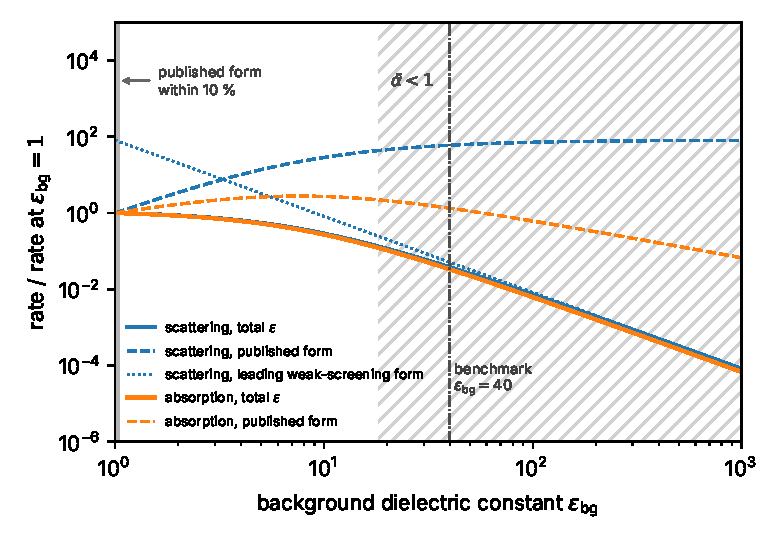
\includegraphics[width=0.9\linewidth]{figures/ch16/limit16_1a.pdf}
\captionof{figure}{Rates of the gapped isotropic Dirac material of Ref.~\cite{hochberg2018detection} ($v_{\mathrm{D}} = 4\times10^{-4}$, $\Delta_{\mathrm{D}} = \SI{2.5}{meV}$, $g_{\mathrm{deg}} = 2$, hard cutoff $\Lambda_{\mathrm{D}} = \SI{0.2}{keV}$) against the background dielectric constant at fixed Dirac parameters, each divided by its value at $\varepsilon_{\mathrm{bg}} = 1$, where the two forms coincide. Blue: scattering at $m_\chi = \SI{100}{keV}$ through a light mediator, \cref{eq:10.2-rate}, with the total $\varepsilon$ (solid), the published form (dashed) and the leading weak-screening form $\Imag\varepsilon_{\mathrm{D}}/\varepsilon_{\mathrm{bg}}^2$ (dotted). Orange: dark-photon absorption at $m_\phi = \SI{50}{meV}$ with the total $\varepsilon$ (solid) and the published form (dashed). Gray: $\varepsilon_{\mathrm{bg}} \le 1.049$, where the published scattering rate is within \SI{10}{\percent} of the total-$\varepsilon$ rate. Hatched: $\tilde\alpha < 1$, $\varepsilon_{\mathrm{bg}} > \alpha/v_{\mathrm{D}} = 18.2$, where one-loop screening is used. Dash-dotted: the published benchmark $\varepsilon_{\mathrm{bg}} = 40$, where the total-$\varepsilon$ scattering rate is 0.74 of its leading form. The dashed curves are $\varepsilon_{\mathrm{bg}}^2$ and $\varepsilon_{\mathrm{bg}}$ times the solid ones.}\label{fig:16-limit-dirac}
\par}
\smallskip
For $\varepsilon_{\mathrm{bg}} > 1$ the published form leaves out the screening of the dark-photon field by the remote bands; at large $\varepsilon_{\mathrm{bg}}$ its scattering rate tends to the unscreened rate of the Dirac pairs, 0.99 of it at $\varepsilon_{\mathrm{bg}} = 1000$, while the true rate falls as $1/\varepsilon_{\mathrm{bg}}^2$.
\end{limitbox}

\begin{workedexample}{The factor $\varepsilon_{\mathrm{bg}}^2$ at $\varepsilon_{\mathrm{bg}} = 40$}\label{we:16-factor}
The ideal Dirac material of Ref.~\cite[Fig.~4]{hochberg2018detection} has $v_{\mathrm{D}} = 4\times10^{-4}$, $\varepsilon_{\mathrm{bg}} = 40$, $g_{\mathrm{deg}} = 2$ and a cutoff of \SI{0.2}{keV}, which we read as a hard cutoff, $v_{\mathrm{D}}\Lambda_{\mathrm{D}} = \SI{80}{meV}$. The coupling is $\tilde\alpha = \alpha/(40\times4\times10^{-4}) = 0.456$, and $g_{\mathrm{deg}}\tilde\alpha = 0.91$ is the effective coupling quoted there.

\emph{One point.} Take the gapless cone at $\vect{q} \to 0$ and $\omega = \SI{10}{meV}$, so that $\sqrt{s} = \SI{10}{meV}$. \Cref{eq:D.22-gapless} gives the bracket $\ln(4v_{\mathrm{D}}^2\Lambda_{\mathrm{D}}^2/s) + \ii\pi = 5.545 + 3.142\ii$, and with $g_{\mathrm{deg}}\alpha/(6\pi v_{\mathrm{D}}) = 1.936$, $\varepsilon_{\mathrm{D}} = 10.73 + 6.08\ii$. The total is $\varepsilon = 50.73 + 6.08\ii$ and $|\varepsilon|^2 = 2611$, so $L = 6.08/2611 = 2.33\times10^{-3}$, 0.61 of the leading form $6.08/1600 = 3.80\times10^{-3}$. Had the \SI{0.2}{keV} been a cutoff in the subtraction scheme of the reference, the bracket would gain $\frac53$, $\Real\varepsilon_{\mathrm{D}}/\varepsilon_{\mathrm{bg}}$ would rise from 0.27 to 0.35, and the ratio to the leading form would be 0.54. The published construction divides $\Imag\varepsilon_{\mathrm{D}} = 6.08$ by $|\varepsilon/\varepsilon_{\mathrm{bg}}|^2 = 1.632$ and obtains 3.73, which is $1600$ times $L$.

\emph{Absorption.} At $m_\phi = \SI{10}{meV}$ the same $\varepsilon$ applies. The published rate is $\zeta^2m_\phi\Imag\varepsilon_{\mathrm{pub}}/|\varepsilon_{\mathrm{pub}}|^2 = 0.0932\,\zeta^2m_\phi$, forty times $\zeta^2m_\phi L$. With the density \SI{10}{g.cm^{-3}} of the reference and $\rho_\chi = \SI{0.3}{GeV.cm^{-3}}$, \cref{eq:10.7-dp} gives $3.35\times10^{30}\,\zeta^2$ events per kg-year, and three events in a kg-year reach $\zeta = 9.5\times10^{-16}$, against $1.5\times10^{-16}$ with the published form, a factor $\sqrt{40} = 6.3$.

\emph{Scattering reach.} For scattering the reference counts one Dirac valence electron per cell, $n_e = \SI{5e24}{kg^{-1}}$ electrons per unit mass in cells of $V_{\mathrm{uc}} = \SI{60}{\angstrom^3}$, which fixes the density $1/(n_eV_{\mathrm{uc}}) = \SI{3.33}{g.cm^{-3}}$; its absorption estimate takes \SI{10}{g.cm^{-3}} instead, and we keep each with its own rate. For the gapped cone ($\Delta_{\mathrm{D}} = \SI{2.5}{meV}$) at $m_\chi = \SI{100}{keV}$, with the standard halo and three events in a kg-year, \cref{eq:10.2-rate} with \cref{eq:16.1-L} reaches $\sigmae = \SI{4.4e-42}{cm^2}$, and the published form $\SI{2.8e-45}{cm^2}$, a factor 1600 at this and at every other mass, 3.2 decades. The published curve for this material has its minimum, \SI{3.4e-46}{cm^2} near \SI{9}{keV}, read from the reference's figure; corrected, it lies at \SI{5.4e-43}{cm^2}.\footnote{The published curve lies about a factor two above the reference's own formula: with the standard halo it reads \SI{5.0e-45}{cm^2} at \SI{100}{keV} against the recomputed \SI{2.8e-45}{cm^2}, a factor 1.8. The factor 1600 between the published and the total-$\varepsilon$ reach holds either way.}
\end{workedexample}

\subsection{ZrTe\texorpdfstring{$_5$}{5} and other anisotropic targets}\label{sec:16.1-zrte5}

Take an anisotropic cone and a background tensor with the same principal axes. The background enters the longitudinal function as $\hat{\vect{q}}\cdot\varepsilon_{\mathrm{bg}}\cdot\hat{\vect{q}} = \sum_i\varepsilon_{\mathrm{bg},ii}\hat q_i^2$. The rescaling at the end of \cref{app:D.22} turns $q^2/v_{\mathrm{D}}$ in the overlap into $\tilde q^2/(v_1v_2v_3)$ with $\tilde{\vect{q}} = (v_1q_1, v_2q_2, v_3q_3)$, so that
\begin{equation}
  \varepsilon(\vect{q},\omega) = \sum_i\varepsilon_{\mathrm{bg},ii}\hat q_i^2 + \sum_i\hat q_i^2\,\varepsilon_{\mathrm{D},i}(\omega^2 - \tilde q^2), \qquad
  \varepsilon_{\mathrm{D},i} = \frac{g_{\mathrm{deg}}\alpha}{6\pi}\,\frac{v_i^2}{v_1v_2v_3}\,B_{\mathrm{D}}(\omega^2 - \tilde q^2) ,
  \label{eq:D.41-aniso}
\end{equation}
with $B_{\mathrm{D}}$ the bracket of \cref{eq:7.3-eps} and $v_{\mathrm{D}}\Lambda_{\mathrm{D}}$ replaced by the energy cutoff $\tilde\Lambda$ of \cref{eq:7.3-aniso}. Both terms of \cref{eq:D.41-aniso} carry the factor $\hat q_i^2$ of a longitudinal function; the background is not divided into the Dirac term. The in-medium factor of Ref.~\cite[Eq.~(3.14)]{geilhufe2020dirac} instead divides each component of the Dirac polarization by its own background constant, $\varepsilon_{\mathrm{pub}} = 1 + \sum_i\hat q_i^2\varepsilon_{\mathrm{D},i}/\varepsilon_{\mathrm{bg},ii}$. The ratio of the two loss functions is
\begin{equation}
  \frac{L_{\mathrm{pub}}}{L} = \frac{|\sum_i\hat q_i^2(\varepsilon_{\mathrm{bg},ii} + \varepsilon_{\mathrm{D},i})|^2}{|1 + \sum_i\hat q_i^2\varepsilon_{\mathrm{D},i}/\varepsilon_{\mathrm{bg},ii}|^2} .
  \label{eq:D.41-ratio}
\end{equation}
(The term of the $x$ axis is read with $q_x^2v_x^2$, where that equation prints $q_x^2v_z^2$.) Along a principal axis the ratio is $\varepsilon_{\mathrm{bg},ii}^2$, which for the computed tensor of ZrTe$_5$, $\varepsilon_{\mathrm{bg},ii} = 308.4$, 20.75 and 126.1~\cite[Table~2]{geilhufe2020dirac}, is $9.5\times10^4$, 431 and $1.6\times10^4$. Off the axes it is not a power of any single background constant: for $\varepsilon_{\mathrm{D}} \to 0$ it tends to $(\hat{\vect{q}}\cdot\varepsilon_{\mathrm{bg}}\cdot\hat{\vect{q}})^2$, and for finite $\varepsilon_{\mathrm{D}}$ it depends on $\hat{\vect{q}}$ through both sums. The event rates then differ by the ratio of their integrals over directions and energies, which the reach of an anisotropic target must be computed with. The background tensor also orders the directions by itself. At equal Dirac numerator, a momentum transfer along $y$, the axis of the smallest background constant, gives a rate $(308.4/20.75)^2 = 221$ times that along $x$. The rate of a crystal fixed in the laboratory therefore modulates daily mainly through its background tensor, which neither a harmonic mean of the tensor nor the per-component factor represents.

We evaluate ZrTe$_5$ with the parameter row that the calculation of \cref{we:7-zrte5} gives for the measured crystal structure~\cite[Table~1 and text below it]{geilhufe2020dirac}: the principal velocities $1.1\times10^{-3}$, $4.5\times10^{-4}$ and $1.0\times10^{-3}$, the energy cutoff $\tilde\Lambda = \min_iv_i\Lambda_i = \SI{0.191}{eV}$, $g_{\mathrm{deg}} = 2$, and the half-gap $\Delta_{\mathrm{D}} = \SI{11.8}{meV}$, half the computed gap of \SI{23.6}{meV}. The relaxed cell of \cref{we:7-zrte5}, the row the reference implements, gives \SI{15.6}{meV} with its own velocities and cutoff, and an earlier calculation \SI{17.5}{meV}. The threshold mass is \SI{8.0}{keV} for the isotropic cone and 9.6, 7.1 and \SI{9.0}{keV} along the principal axes. We average the loss function over the directions of $\vect{q}$, which gives the rate averaged over the orientations of the crystal relative to the dark-matter wind, and insert it into \cref{eq:10.2-rate} with a light mediator, the standard halo and the measured density \SI{6.089}{g.cm^{-3}}~\cite[Fig.~3]{geilhufe2020dirac}. At $m_\chi = \SI{100}{keV}$ and $\sigmae = \SI{e-38}{cm^2}$ this yields 108 events per kg-year. Since a background-free reach scales as the inverse rate (\cref{eq:1.5-limscaling}), three events in a kg-year reach about \SI{1.5e-40}{cm^2} near \SI{40}{keV} (\cref{fig:16-zrte5}a). The published rule, recomputed with the same inputs and the standard halo, gives a rate 5200 to 6400 times larger between \SI{20}{keV} and \SI{1}{MeV}. Over the two computed rows (11.8 and \SI{15.6}{meV}) and the two halos of \cref{fig:16-zrte5} the factor spans 4800 to 6600, and a halo with $v_0 = 220$, $v_{\mathrm{E}} = 232$ and $v_{\mathrm{esc}} = \SI{544}{km.s^{-1}}$ lowers its lower end to 4300. That is more than the square of the harmonic mean of the tensor, $50.5^2 = 2550$, and an isotropic model of the same row, with the geometric-mean velocity and the harmonic-mean background as in \cref{we:7-zrte5}, overstates the orientation-averaged total-$\varepsilon$ rate by a factor 2.3 to 2.7. The curve of Hochberg et al.~\cite{hochberg2018detection}, computed for an isotropic model with $\varepsilon_{\mathrm{bg}} = 25.34$, the harmonic mean of its own tensor (187.5, 9.8 and 90.9), moves by $25.34^2 = 642$ exactly.

\begin{figure}[tbp]
  \centering
  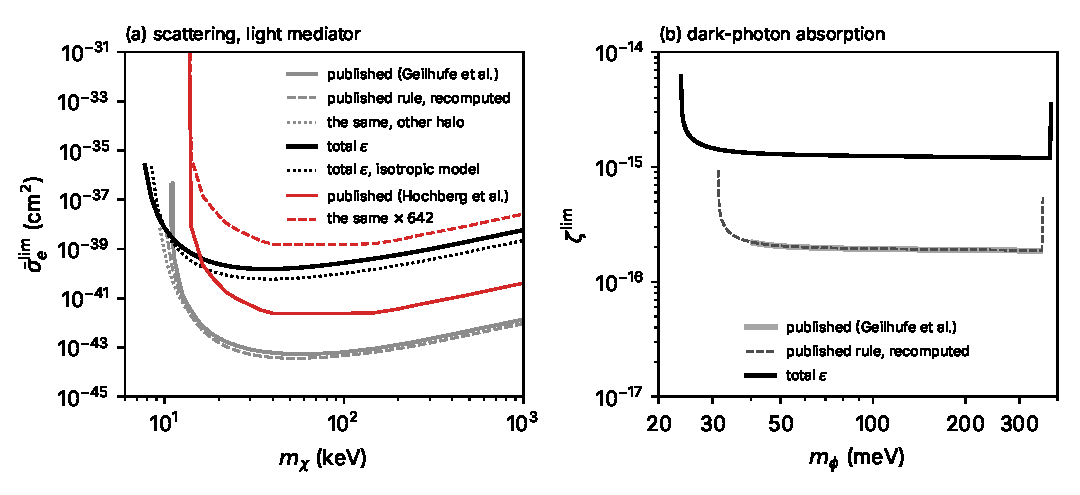
\includegraphics[width=\linewidth]{figures/ch16/fig16_1.pdf}
  \caption{ZrTe$_5$ reach as published and with the background in the total dielectric function: three events in one kg-year, no background, $\rho_\chi = \SI{0.3}{GeV.cm^{-3}}$. (a) Scattering through a light mediator. Gray solid: the published curve for the computed parameters of Geilhufe et al.~\cite{geilhufe2020dirac} (read from their figure). Gray dashed: their in-medium factor, recomputed for their half-gap, \SI{15.6}{meV}, with the standard halo and the loss function averaged over the directions of $\vect{q}$; it lies at 0.63 to 0.72 of the published curve above \SI{20}{keV}, consistent with a difference of halo: the source states none, and with $v_0 = 220$, $v_{\mathrm{E}} = 232$ and $v_{\mathrm{esc}} = \SI{600}{km.s^{-1}}$ (gray dotted) the ratio is 0.8 to 1.1. Black solid: the target with the total $\varepsilon$, \cref{eq:16.1-L} with the anisotropic $\varepsilon_{\mathrm{D}}$ of \cref{eq:D.41-aniso}, measured-structure row ($\Delta_{\mathrm{D}} = \SI{11.8}{meV}$, $\tilde\Lambda = \SI{0.191}{eV}$), density \SI{6.089}{g.cm^{-3}}. Black dotted: its isotropic model (geometric-mean velocity, harmonic-mean $\varepsilon_{\mathrm{bg}} = 50.5$) with the total $\varepsilon$. Red: the published curve of Hochberg et al.~\cite{hochberg2018detection} for their ZrTe$_5$ parameters, isotropized with $\varepsilon_{\mathrm{bg}} = 25.34$ (solid), and the same curve times 642 (dashed). (b) Absorption of dark-photon dark matter, each polarization along a principal axis, unpolarized average, density \SI{6.135}{g.cm^{-3}} as in Ref.~\cite{geilhufe2020dirac}. Gray: their published curve; dashed: their rule recomputed with $\Delta_{\mathrm{D}} = \SI{15.6}{meV}$, within \SI{0.5}{\percent} of it; black: the total $\varepsilon$ with the measured-structure row. Published-rule curves: $\Delta_{\mathrm{D}} = \SI{15.6}{meV}$, $\tilde\Lambda = \SI{0.180}{eV}$. Off-diagonal entries of the tensor ($|\varepsilon_{\mathrm{bg},ij}| \le 1.2$) are dropped.}
  \label{fig:16-zrte5}
\end{figure}

Absorption at rest has no direction of $\vect{q}$, but the polarization of the dark photon picks a component of the tensor, and each polarization is absorbed with the factor $\varepsilon_{\mathrm{bg},ii}$ of \cref{eq:16.1-ratio}. With the total $\varepsilon$ the polarization along $y$, with the smallest background constant, carries \SI{86}{\percent} of the unpolarized rate at \SI{100}{meV}. Recomputed with the published rule, our absorption rate reproduces the published reach of Ref.~\cite{geilhufe2020dirac} to \SI{0.5}{\percent} over the whole range, which checks the inputs. With the total $\varepsilon$ and the measured-structure row, the reach in $\zeta$ weakens by a factor of 6.3 to 6.4 between the gap and the cutoff (\cref{fig:16-zrte5}b), to about $1.25\times10^{-15}$ at \SI{100}{meV}. The factor is the square root of a polarization average and lies between $\varepsilon_{\mathrm{bg},yy}^{1/2} = 4.6$ and $\varepsilon_{\mathrm{bg},xx}^{1/2} = 17.6$. For the cubic Yb$_3$PbO of the same reference the factors are $42.8^2 = 1832$ and $42.8^{1/2} = 6.5$ identically. Its computed dielectric constant, however, is described there as sensitive to the size of the gap~\cite[Sect.~4]{geilhufe2020dirac}. It contains the Dirac bands, the background is smaller than 42.8, and the Dirac term is counted twice under either rule. These two factors describe the model, not the material.

\subsection{Excitonic and strong-coupling corrections}\label{sec:16.1-validity}

\Cref{eq:16.1-L} keeps the random-phase response of the Dirac electrons, the first order in $\tilde\alpha$ of their polarization, with the expansion parameter $g_{\mathrm{deg}}\tilde\alpha\ln[v_{\mathrm{D}}\Lambda_{\mathrm{D}}/\max(\Delta_{\mathrm{D}}, v_{\mathrm{D}}q)]$ of \cref{sec:7.3}. For ZrTe$_5$ that is 1.02 at long wavelength with the measured-structure row (0.93 with the relaxed cell), at the edge of the expansion, and for the benchmark of \cref{we:16-factor}, $g_{\mathrm{deg}}\tilde\alpha = 0.91$ times a logarithm of a few. At next order the electron--hole ladder, the self-energy and vertex of the carriers, and the material outside the model all enter.

The ladder of the Bethe--Salpeter equation (\cref{sec:4.9}) is the attraction between the electron and the hole of a pair. Near the edge the pair is nonrelativistic, with reduced mass $\Delta_{\mathrm{D}}/2v_{\mathrm{D}}^2$ and Coulomb coupling $\alpha/\varepsilon_{\mathrm{bg}}$. It binds with the energy $(\Delta_{\mathrm{D}}/2v_{\mathrm{D}}^2)(\alpha/\varepsilon_{\mathrm{bg}})^2/2 = \Delta_{\mathrm{D}}\tilde\alpha^2/4$, \SI{0.10}{meV} for the isotropic model of ZrTe$_5$ with $\tilde\alpha = 0.18$, and its continuum carries the Sommerfeld factor $x/(1 - \ee^{-x})$ with $x = \pi\tilde\alpha/b$. Here $b = (1 - 4\Delta_{\mathrm{D}}^2/s)^{1/2}$ is the speed of each carrier in the rest frame of the pair, in units of $v_{\mathrm{D}}$. In ZrTe$_5$ the factor exceeds 1.5 for $b < 0.66$, that is for pair energies up to 1.33 times the edge, and that region carries \SI{60}{\percent} of the rate at \SI{20}{keV}, \SI{12}{\percent} at \SI{100}{keV} and \SI{3}{\percent} at \SI{1}{MeV} in the isotropic model. Near the threshold mass the reach is therefore uncertain by the Sommerfeld factor, 1.5 or more, until the ladder is solved, which \cref{app:E.20} specifies. The bound states lie at $\sqrt{s} < 2\Delta_{\mathrm{D}}$ and add absorption lines below the edge.

The self-energy of the carriers renormalizes $v_{\mathrm{D}}$ logarithmically in the cutoff, and a vertex correction accompanies it. Each is of relative order $\tilde\alpha$, with a coefficient that the one-loop result does not fix. Outside the model, a chemical potential inside a band adds an intraband term, Thomas--Fermi screening with $k_{\mathrm{TF}}^2 = e^2\mathcal{N}_{\mathrm{D}}(E_{\mathrm{F}})/\varepsilon_{\mathrm{bg}}$, which removes the weak screening at $\omega \lesssim v_{\mathrm{D}}k_{\mathrm{F}}$. The background acquires ionic poles near the optical phonons. And the bands bend beyond $\Lambda_{\mathrm{D}}$, which moves weight between the background and the logarithm of \cref{eq:7.3-static}.

At $\tilde\alpha \gtrsim 1$ none of these is small, and no controlled method is known. The ladder is the controlled correction of first order in $\tilde\alpha$ and is uncontrolled beyond it; neither self-consistent $GW$ with the Bethe--Salpeter equation nor a functional renormalization group has a small parameter there. The question matters for the slowest cones, which have the most states and the lowest thresholds. BNQ-TTF, with velocities near $2\times10^{-4}$, has an effective coupling of about 10, and its authors present its one-loop rates as a qualitative estimate~\cite[footnote~3]{geilhufe2020dirac}. What replaces \cref{eq:16.1-L} for such targets is open.

\section{Low-dimensional plasmons and layered stacks}\label{sec:16.2}

Rolled into a metallic carbon nanotube, the Dirac electrons of \cref{sec:16.1} put their whole low-energy response to a density coupling into one line, $\omega = v_{\mathrm{D}}q_\parallel/g_c$, with $v_{\mathrm{D}} = 3.02\times10^{-3}$ the Dirac velocity of graphene. The Luttinger parameter $g_c \approx 0.2$ (\cref{eq:16.2-wire}) makes the line 3.4 to 6.9 times faster than any particle of the halo at momenta of 1 to \SI{100}{eV}. The plasmon of a doped graphene sheet is faster still at the momenta of keV-mass dark matter. In bulk silicon a mode that fast is out of reach: the plasmon of \cref{sec:10.3} needs a particle at \SI{2860}{km.s^{-1}}. In a tube or a sheet, however, the response depends only on the momentum along the tube or in the plane, and a halo particle can supply the rest of its momentum across it. A mode faster than $v_{\mathrm{max}}$ is then reached by an oblique momentum transfer, and the confined plasmon becomes a final state of its own. Its weight sits in a single line at low energy, which is what the sum-rule bounds of \cref{sec:10.2} need to come close to saturation. We will derive the Coulomb kernels of sheets and tubes, the random-phase plasmons in one and two dimensions, the acoustic plasmon of two kinds of carriers, and the dielectric function of a stack of layers, exact at long wavelength, with its leading correction.

\subsection{Confined electrons and their Coulomb kernels}\label{sec:16.2-kernels}

Consider identical units, wires or sheets, in which electrons move freely in one or two dimensions and are confined across, with no tunneling between units. Write $\vect{q} = (\vect{q}_\parallel, \vect{q}_\perp)$, with $\vect{q}_\parallel$ along the free directions. Suppose the distribution of the electrons across a unit does not depend on their state along it. The density operator of \cref{eq:2.3-nq} then factorizes, $n_e(\vect{q}) = \sum_u \ee^{\ii\vect{q}_\perp\cdot\vect{r}_u}F_\perp(\vect{q}_\perp)\,n_u(\vect{q}_\parallel)$. Here $\vect{r}_u$ locates unit $u$, $n_u$ is its density operator along the free directions, and the transverse form factor $F_\perp$ is the Fourier transform of the normalized distribution across the unit, with $F_\perp(0) = 1$. For a sheet of uniform thickness $d$, $F_\perp = \sin(q_zd/2)/(q_zd/2)$; for a tube whose electrons sit on a cylinder of radius $r_{\mathrm{t}}$, $F_\perp = J_0(q_\perp r_{\mathrm{t}})$. If the units respond independently, the cross terms between units average to zero at $\omega \ne 0$. The structure factor of \cref{eq:4.2-Sab} then becomes
\begin{equation}
  S(\vect{q},\omega) = \nd_{\mathrm{u}}\,|F_\perp(\vect{q}_\perp)|^2\,S_{\mathrm{u}}(\vect{q}_\parallel,\omega) ,
  \label{eq:16.2-embed}
\end{equation}
with $\nd_{\mathrm{u}}$ the number of units per unit transverse area (wires) or length (sheets) and $S_{\mathrm{u}}$ the structure factor of one unit per unit length or area, in the normalization of \cref{sec:4.2}. In \cref{eq:8.2-spectrum} the target enters as $S/\rho_T = |F_\perp|^2S_{\mathrm{u}}/\rho_{\mathrm{u}}$, with $\rho_{\mathrm{u}}$ the mass of one unit per unit length or area. The rate per unit mass is then independent of how densely the units are packed, as long as they remain independent. The tube proposal of Zhang and Chen reports its rate per unit tube length~\cite[Eq.~(6)]{zhang2026luttinger}, and Das, Jang and Min write \cref{eq:16.2-embed} for a sheet of uniform thickness with the areal mass density~\cite[Eqs.~(13), (14)]{das2023sub}.

\Cref{eq:16.2-embed} changes the kinematics. The structure factor depends on $\vect{q}_\parallel$ alone, while the dark matter deposits $\omega = \vect{q}\cdot\vect{v} - q^2/2\mchi$ with the full $\vect{q}$. A mode at $(\vect{q}_\parallel, \omega)$ is reached by any $\vect{q}$ with that projection, and the condition $\omega \le qv_{\mathrm{max}} - q^2/2\mchi$ only requires $q \gtrsim \omega/v_{\mathrm{max}}$, which can exceed $q_\parallel$ by any amount. The cost is the form factor, which falls once $q_\perp$ exceeds the inverse thickness. For a tube of radius \SI{0.7}{nm}, $|J_0|^2$ starts to fall at $q_\perp \approx 1/r_{\mathrm{t}} = \SI{282}{eV}$, and halo particles reach energies up to $v_{\mathrm{max}}/r_{\mathrm{t}} = \SI{0.75}{eV}$ without that suppression. A bulk mode at $(\vect{q},\omega)$, by contrast, is reached only if $\omega \le qv_{\mathrm{max}}$ at its own $\vect{q}$.

The electrons of a unit interact through the Coulomb potential averaged over the transverse distribution. Take a sheet between two half spaces of dielectric constants $\varepsilon_a$ and $\varepsilon_b$. \Cref{sec:15.3-sheet} found the potential of its density wave from the two-dimensional Fourier transform of $e^2/4\pi r$ and the image charges,
\begin{equation}
  v_{\mathrm{C}}^{\mathrm{2D}}(q_\parallel) = \frac{e^2}{(\varepsilon_a + \varepsilon_b)\,q_\parallel} = \frac{e^2}{2\bar\varepsilon\,q_\parallel} ,
  \qquad
  \varepsilon_{\mathrm{2D}} = 1 - v_{\mathrm{C}}^{\mathrm{2D}}\tilde R^{\mathrm{2D}} ,
  \qquad
  S_{\mathrm{2D}} = -2\,\Imag\frac{\tilde R^{\mathrm{2D}}}{\varepsilon_{\mathrm{2D}}} \quad (T = 0) ,
  \label{eq:16.2-kernel2D}
\end{equation}
with $\bar\varepsilon = (\varepsilon_a + \varepsilon_b)/2$ and $\tilde R^{\mathrm{2D}}$ the proper density response of the sheet per unit area, the two-dimensional analogue of \cref{eq:4.4-proper}. The kernel falls as $1/q_\parallel$, not as $1/q^2$: a sheet screens a long-wavelength potential weakly, because the field of its induced charge spreads into the space around it. Give the sheet a finite thickness $d$, with a uniform distribution across it in a homogeneous medium. Averaging $\ee^{-q_\parallel|z - z'|}$ over both positions multiplies the kernel by
\begin{equation}
  F_{\mathrm{th}}(q_\parallel d) = \frac{2}{q_\parallel d} - \frac{2\bigl(1 - \ee^{-q_\parallel d}\bigr)}{(q_\parallel d)^2} = 1 - \frac{q_\parallel d}{3} + O\bigl(q_\parallel^2d^2\bigr) .
  \label{eq:16.2-thick}
\end{equation}
For the interlayer distance $d = \SI{3.35}{\angstrom}$ of bilayer graphene the factor is 0.95 at $q_\parallel = \SI{100}{eV}$ and 0.85 at \SI{300}{eV}, and it reaches 0.9 at \SI{191}{eV}; Ref.~\cite[Eq.~(17)]{das2023sub} keeps the profile in the form factor but uses the zero-thickness kernel, a correction of this size at the momenta of sub-MeV dark matter.

The bands far from the Fermi level enter the proper response as a static part $\tilde R^{\mathrm{2D}}_{\mathrm{bg}}$, which for an insulating background is proportional to $q_\parallel^2$ at small $q_\parallel$. Writing $-\tilde R^{\mathrm{2D}}_{\mathrm{bg}} = 2r_0q_\parallel^2/e^2$ defines the Keldysh length $r_0$, and
\begin{equation}
  \bar\varepsilon\,\varepsilon_{\mathrm{2D}}(q_\parallel,\omega) = \bar\varepsilon + r_0q_\parallel - \frac{e^2}{2q_\parallel}\,\tilde R^{\mathrm{2D}}_{\mathrm{low}}(q_\parallel,\omega) ,
  \label{eq:16.2-keldysh}
\end{equation}
with $\tilde R^{\mathrm{2D}}_{\mathrm{low}}$ the response of the bands near the Fermi level. Compared to a bulk material, the remote bands of a sheet do not screen at long wavelength: their contribution $r_0q_\parallel$ vanishes as $q_\parallel \to 0$, while in three dimensions they give the constant $\varepsilon_{\mathrm{bg}}$ of \cref{sec:7.3} that \cref{sec:16.1} places inside the total $\varepsilon$. In a sheet the substrate enters only through $\bar\varepsilon$ and the remote bands only through $r_0$; neither rescales the coupling to the dark matter. A polar substrate makes $\varepsilon_b$ depend on frequency, and the sheet plasmon then mixes with its surface phonons.

For a tube the same average over a cylindrical shell of radius $r_{\mathrm{t}}$ selects the azimuthally uniform term of the expansion of $1/|\vect{r} - \vect{r}'|$ in cylindrical coordinates, $(2/\pi)\int_0^\infty\dd k\cos[k(z - z')]I_0(kr_{\mathrm{t}})K_0(kr_{\mathrm{t}})$, with $I_0$ and $K_0$ the modified Bessel functions of order zero~\cite[Sect.~10.25]{olver2010nist}. Its Fourier transform along the axis is $2I_0(q_\parallel r_{\mathrm{t}})K_0(q_\parallel r_{\mathrm{t}})$, and with $e^2 = 4\pi\alpha$ (\cref{app:A.2})
\begin{equation}
  v_{\mathrm{C}}^{\mathrm{1D}}(q_\parallel) = \frac{2\alpha}{\varepsilon_{\mathrm{env}}}\,I_0(q_\parallel r_{\mathrm{t}})\,K_0(q_\parallel r_{\mathrm{t}}) \simeq \frac{2\alpha}{\varepsilon_{\mathrm{env}}}\Bigl[\ln\frac{2}{q_\parallel r_{\mathrm{t}}} - \gamma_{\mathrm{E}}\Bigr] \quad (q_\parallel r_{\mathrm{t}} \ll 1) ,
  \label{eq:16.2-kernel1D}
\end{equation}
for a tube in a medium of dielectric constant $\varepsilon_{\mathrm{env}}$, with $\gamma_{\mathrm{E}}$ Euler's constant; the small-argument form follows from $I_0 \to 1$ and $K_0(x) \to \ln(2/x) - \gamma_{\mathrm{E}}$~\cite[Eqs.~(10.30.1), (10.31.2)]{olver2010nist}. The logarithmic form falls \SI{10}{\percent} below the exact kernel at $q_\parallel r_{\mathrm{t}} = 0.38$, which is \SI{108}{eV} for $r_{\mathrm{t}} = \SI{0.7}{nm}$. The logarithm comes from the one-dimensional geometry: the interaction of two lines of charge grows without bound as their wavelength grows.

\Cref{app:E.21} specifies how $\tilde R^{\mathrm{2D}}$, $r_0$ and the corresponding tables for tubes and stacks are computed. The proper response of a monolayer comes from a plane-wave code with the Coulomb interaction cut off between periodic images, or from a Wannier-function bubble. The substrate enters through its measured $\varepsilon_b(\omega)$ with the polar phonons, and the random-phase equations are solved with the kernels above.

\subsection{Plasmons in one and two dimensions}\label{sec:16.2-plasmons}

At frequencies above the pair continuum the proper response of any band takes the form $\tilde R \simeq D_{\mathrm{Dr}}\,q_\parallel^2/\omega^2$, with $D_{\mathrm{Dr}}$ the Drude weight. The coefficient follows from the intraband part of the Lehmann sum, expanded for $\omega \gg \vect{q}\cdot\vect{v}$: $D_{\mathrm{Dr}} = \sum_{\vect{k}}(-\partial n_{\mathrm{F}}/\partial E)(\hat{\vect{q}}\cdot\vect{v}_{\vect{k}})^2$ per unit area, summed over spin and valleys. For a parabolic band of mass $m^*$ this is $\nd_{\mathrm{2D}}/m^*$, the areal density over the mass, as the $f$-sum rule requires. For a Dirac cone, $\vect{v}_{\vect{k}} = v_{\mathrm{D}}\hat{\vect{k}}$ and the Fermi circle has length $2\pi k_{\mathrm{F}}$, so $D_{\mathrm{Dr}} = g_{\mathrm{deg}}E_{\mathrm{F}}/4\pi$, with $g_{\mathrm{deg}} = 4$ for graphene. The zero of $\varepsilon_{\mathrm{2D}}$ in \cref{eq:16.2-kernel2D} is then the sheet plasmon. For a parabolic band the next term of the high-frequency expansion is that of \cref{eq:4.5-moments}, with the disc average $\langle(\hat{\vect{q}}\cdot\vect{v})^2\rangle = v_{\mathrm{F}}^2/4$ in place of the sphere's $v_{\mathrm{F}}^2/5$. Then
\begin{equation}
  \omega_{\mathrm{pl}}^2(q_\parallel) = \frac{e^2\,\nd_{\mathrm{2D}}\,q_\parallel}{(\varepsilon_a + \varepsilon_b)\,m^*} + \frac34\,v_{\mathrm{F}}^2q_\parallel^2 + O\bigl(q_\parallel^3\bigr) .
  \label{eq:16.2-2Dpl}
\end{equation}
Compared to the bulk plasmon, which starts at $\omega_p$, the sheet plasmon is gapless and rises as $\sqrt{q_\parallel}$, because the kernel falls only as $1/q_\parallel$. It stays undamped as long as it lies above the pair continuum, $\omega > q_\parallel v_{\mathrm{F}} + q_\parallel^2/2m^*$. For doped graphene in vacuum, $\omega_{\mathrm{pl}}^2 = 2\alpha E_{\mathrm{F}}q_\parallel$. At $E_{\mathrm{F}} = \SI{0.2}{eV}$ its phase velocity is 20 times $v_{\mathrm{max}}$ at $q_\parallel = \SI{1}{eV}$ and 6.4 times at \SI{10}{eV}, and the long-wavelength form ends at $q_\parallel = \SI{32}{eV}$, where $\omega = \SI{0.30}{eV}$ and the line meets the interband edge $2E_{\mathrm{F}} - v_{\mathrm{D}}q_\parallel$. Here $v_{\mathrm{D}} = 3ta_{\mathrm{cc}}/2 = 3.02\times10^{-3}$, from the nearest-neighbor hopping $t = \SI{2.8}{eV}$ and the carbon--carbon distance $a_{\mathrm{cc}} = \SI{1.42}{\angstrom}$~\cite[text after Eqs.~(5) and (7)]{castroneto2009electronic}, the value used for graphene and nanotubes throughout this chapter. Das, Jang and Min quote a hopping of \SI{3.16}{eV} for their bilayer model~\cite[Sect.~II]{das2023sub}, and Zhang and Chen take $v = \SI{0.8e6}{m.s^{-1}} = 2.67\times10^{-3}$ for nanotubes~\cite{zhang2026luttinger}. Their rate for bilayer graphene is \cref{eq:16.2-embed,eq:16.2-kernel2D} at $\varepsilon_a = \varepsilon_b = 1$, with the random-phase response of the four low-energy bands~\cite[Eqs.~(13)--(19)]{das2023sub}; on a substrate the 2 in their kernel $e^2/2q$ becomes $\varepsilon_a + \varepsilon_b$. Their gate opens a gap and puts the Fermi level inside it, so their loss function is interband and has no sheet plasmon.

The bands of a metallic nanotube at its Fermi level are linear. The tube has $N_{\mathrm{ch}}$ channels at the Fermi level, two for spin times two for the valleys, each with right- and left-moving electrons of velocity $\pm v$; for a nanotube $v = v_{\mathrm{D}}$. For the right movers of one channel, $n_k - n_{k+q} = 1$ on an interval of length $q$ below $k_{\mathrm{F}}$ and the energy denominator is $\omega - vq$; the left movers give the same with $-v$. Their sum per unit length is $(q/2\pi)[1/(\omega - vq) - 1/(\omega + vq)]$, and for $N_{\mathrm{ch}}$ channels
\begin{equation*}
  R^0_{\mathrm{1D}}(q_\parallel,\omega) = \frac{N_{\mathrm{ch}}\,v\,q_\parallel^2}{\pi\,(\omega^2 - v^2q_\parallel^2)} .
\end{equation*}
The random-phase response $R = R^0_{\mathrm{1D}}/(1 - v_{\mathrm{C}}^{\mathrm{1D}}R^0_{\mathrm{1D}})$ has its pole where $\omega^2 = v^2q_\parallel^2[1 + N_{\mathrm{ch}}v_{\mathrm{C}}^{\mathrm{1D}}/(\pi v)]$, and near it $\Imag[1/(\omega^2 - \omega_{\mathrm{pl}}^2 + \ii0^+)] = -\pi\delta(\omega - \omega_{\mathrm{pl}})/2\omega_{\mathrm{pl}}$, so that $S = -2\Imag R$ is a single line:
\begin{keyresult}[One-dimensional plasmon of linear channels]
\begin{equation}
  S_{\mathrm{1D}}(q_\parallel,\omega) = N_{\mathrm{ch}}\,g_c\,|q_\parallel|\,\delta\Bigl(\omega - \frac{v|q_\parallel|}{g_c}\Bigr) , \qquad
  g_c(q_\parallel) = \Bigl[1 + \frac{N_{\mathrm{ch}}\,v_{\mathrm{C}}^{\mathrm{1D}}(q_\parallel)}{\pi v}\Bigr]^{-1/2} ,
  \label{eq:16.2-wire}
\end{equation}
at $T = 0$ and $\omega > 0$, with $v_{\mathrm{C}}^{\mathrm{1D}}$ of \cref{eq:16.2-kernel1D}. It is embedded in three dimensions by \cref{eq:16.2-embed} with $F_\perp = J_0(q_\perp r_{\mathrm{t}})$.
\end{keyresult}
\noindent For a single channel this is the result of Zhang and Chen~\cite[Eqs.~(3), (4)]{zhang2026luttinger}. They bosonize a model with forward couplings $g_2$ and $g_4$ between right and left movers; with $g_2 = g_4 = v_{\mathrm{C}}^{\mathrm{1D}}$ their Luttinger parameter and velocity become $g_c$ and $v/g_c$ of \cref{eq:16.2-wire}. For this model the random-phase result is exact, because the linear band makes every higher-order term in the interaction cancel; that is the content of bosonization. The product of the weight and the velocity, $g_c\cdot v/g_c = v$, does not depend on the interaction. The first moment of the line, $\int\dd\omega\,\omega S_{\mathrm{1D}} = N_{\mathrm{ch}}vq_\parallel^2$, is therefore that of the free channels, the $f$-sum of the linear bands: the interaction raises the line and lowers its weight in the same proportion.

The charge of a nanotube is carried by all four channels together. The dark matter couples to the total density $n = \sum_in_i$, and so does the Coulomb interaction. The symmetric combination of the channel densities is the plasmon of \cref{eq:16.2-wire} with $N_{\mathrm{ch}} = 4$. The three other combinations, in which spin or valley densities oscillate against each other, carry no charge, keep $g = 1$, and do not appear in $S$. The model of Ref.~\cite{zhang2026luttinger} has one right- and one left-moving mode, $N_{\mathrm{ch}} = 1$, but its benchmark values $g = 0.2$ to 0.7 are those measured for nanotubes, which belong to the charge mode $g_c$ of the four-channel theory. At fixed $g_c$ its structure factor, and the rate of its Eq.~(6), are four times too low. At a fixed interaction instead the comparison is $N_{\mathrm{ch}}g_c(N_{\mathrm{ch}})$ against $g_c(1)$: with the kernel of a tube of radius \SI{0.7}{nm} in vacuum, $g_c = 0.212$ for four channels and 0.398 for one at $q_\parallel = \SI{10}{eV}$, and the four-channel line is 2.1 times stronger.

The interaction is strong. With $r_{\mathrm{t}} = \SI{0.7}{nm}$, $\varepsilon_{\mathrm{env}} = 1$ and the graphene velocity, $N_{\mathrm{ch}}v_{\mathrm{C}}^{\mathrm{1D}}/\pi v_{\mathrm{D}}$ is 35 at $q_\parallel = \SI{1}{eV}$ and 8 at \SI{100}{eV}, and $g_c$ is 0.17, 0.21 and 0.34 at 1, 10 and \SI{100}{eV}, inside the measured range. The plasmon then moves at 6.9, 5.4 and 3.4 times $v_{\mathrm{max}}$. A bulk mode that fast would be unreachable; the line of a tube is reached by any halo particle that deposits $\omega$ with a total momentum $q \gtrsim \omega/v_{\mathrm{max}}$ and a projection $q_\parallel = g_c\omega/v$ on the axis. The rate depends on the angle between the tube and the velocity of the particle, and with it on the time of day, which is the directional signal of Ref.~\cite{zhang2026luttinger}. \Cref{fig:16-dispersion} compares the plasmons of a tube, a sheet and bulk silicon with the reach of the halo.

\begin{figure}[tbp]
  \centering
  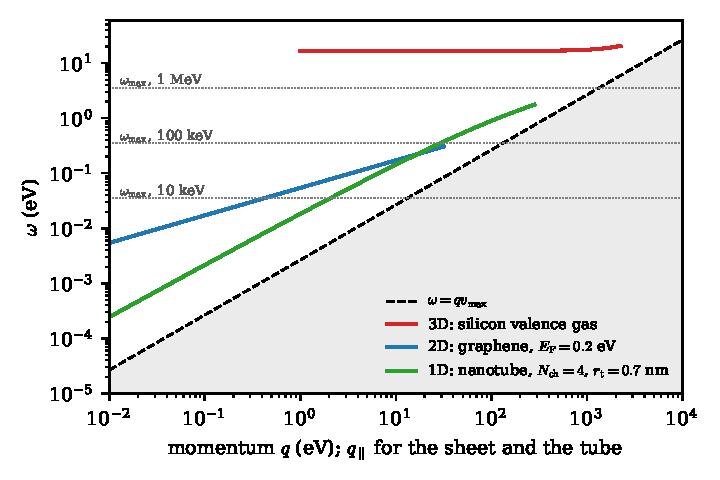
\includegraphics[width=0.85\linewidth]{figures/ch16/fig16_2.pdf}
  \caption{Plasmons in three, two and one dimensions against the reach of halo dark matter. Red: the valence-electron gas of silicon, $\omega_{\mathrm{pl}}^2 = \omega_p^2 + \tfrac35v_{\mathrm{F}}^2q^2$ with $\omega_p = \SI{16.6}{eV}$, to the quadratic cutoff at \SI{2.24}{keV}. Blue: doped graphene in vacuum at a Fermi energy of \SI{0.2}{eV}, $\omega_{\mathrm{pl}}^2 = 2\alpha E_{\mathrm{F}}q_\parallel$, up to the interband edge at \SI{32}{eV}. Green: the charge mode of a metallic nanotube, \cref{eq:16.2-wire} with $N_{\mathrm{ch}} = 4$, $r_{\mathrm{t}} = \SI{0.7}{nm}$, $\varepsilon_{\mathrm{env}} = 1$ and $v_{\mathrm{D}} = 3.02\times10^{-3}$, to $q_\parallel = 1/r_{\mathrm{t}}$. Dashed: $\omega = qv_{\mathrm{max}}$, the largest energy a halo particle deposits with momentum $q$ (gray below it). Dotted: the largest energy $\mchi v_{\mathrm{max}}^2/2$ for three masses. The bulk mode lies above the dashed line at its own $q$ and is out of reach. The modes of the sheet and the tube depend only on $q_\parallel$, and a particle reaches them with a total momentum $q \ge \omega/v_{\mathrm{max}}$, the rest of it across the sheet or the tube.}
  \label{fig:16-dispersion}
\end{figure}

\Cref{eq:16.2-wire} rests on the linear band. A real band curves on the scale of its Fermi momentum, and the limit check below compares the linear channels with parabolic ones of the same velocity $v$ at $k_{\mathrm{F}}$, of mass $m^* = k_{\mathrm{F}}/v$. The one-dimensional Lindhard function of one such channel is $(m^*/2\pi q_\parallel)\ln[(\omega^2 - \omega_-^2)/(\omega^2 - \omega_+^2)]$, with $\omega_\pm = q_\parallel v \pm q_\parallel^2/2m^*$ the edges of its pair band, and the zero of the random-phase dielectric function has the closed form $\omega^2 = (\omega_+^2\ee^{y} - \omega_-^2)/(\ee^{y} - 1)$, with $y = 2\pi q_\parallel/(N_{\mathrm{ch}}v_{\mathrm{C}}^{\mathrm{1D}}m^*)$. Expanding it in $y$, the $q_\parallel^3$ terms cancel and the plasmon frequency is
\begin{equation*}
  \frac{\omega_{\mathrm{pl}}^{\mathrm{par}}}{\omega_{\mathrm{pl}}} = 1 + \frac{q_\parallel^2}{2k_{\mathrm{F}}^2}\,g_c^2\Bigl[\frac14 + \frac{g_c^2}{3(1 - g_c^2)}\Bigr] + O\bigl(q_\parallel^4/k_{\mathrm{F}}^4\bigr) .
\end{equation*}
The correction carries $g_c^2$: the stronger the interaction, the further the plasmon lies above the pairs, and the less the shape of the band matters. In a nanotube the linear band itself ends at the next subbands, whose pairs open at $2v_{\mathrm{D}}/r_{\mathrm{t}} = \SI{1.7}{eV}$; below that energy and for $q_\parallel \ll 1/r_{\mathrm{t}}$ the four channels are the whole low-energy response. In a forest of parallel tubes the Coulomb interaction between tubes adds to $v_{\mathrm{C}}^{\mathrm{1D}}$ once $q_\perp$ is below the inverse spacing, 1 to \SI{2}{eV} for the spacings of 100 to \SI{200}{nm} that Ref.~\cite{zhang2026luttinger} considers.

\begin{limitbox}[One-dimensional plasmons of linear channels][lim:16.2a]
$S_{\mathrm{1D}} = N_{\mathrm{ch}}g_c|q_\parallel|\delta(\omega - v|q_\parallel|/g_c)$ with $g_c = [1 + N_{\mathrm{ch}}v_{\mathrm{C}}^{\mathrm{1D}}/\pi v]^{-1/2}$; Zhang and Chen give the case $N_{\mathrm{ch}} = 1$, and a metallic nanotube has $N_{\mathrm{ch}} = 4$~\cite[Eqs.~(3)--(6)]{zhang2026luttinger}.
\par\smallskip
{\centering
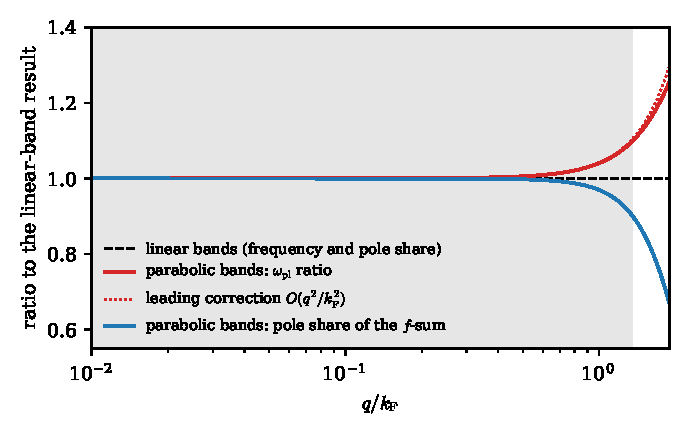
\includegraphics[width=0.82\linewidth]{figures/ch16/limit16_2a.pdf}
\captionof{figure}{Plasmon frequency and pole share of the $f$-sum for $N_{\mathrm{ch}} = 4$ parabolic channels, relative to the linear-band result, against $q_\parallel/k_{\mathrm{F}}$. Both use the kernel of a tube of radius \SI{0.7}{nm} in vacuum and the velocity $v_{\mathrm{D}} = 3.02\times10^{-3}$ at $k_{\mathrm{F}}$; the parabolic band, of mass $k_{\mathrm{F}}/v_{\mathrm{D}}$ with $k_{\mathrm{F}} = 1/r_{\mathrm{t}} = \SI{282}{eV}$, is a model for the curvature that the subbands bring on that scale. Red: frequency ratio; dotted, its leading correction in $q_\parallel^2/k_{\mathrm{F}}^2$. Blue: share of the $f$-sum $N_{\mathrm{ch}}vq_\parallel^2$ in the plasmon line (one for linear bands). Gray: both within \SI{10}{\percent} of the linear-band result, $q_\parallel < 1.36\,k_{\mathrm{F}}$. Along the curve $g_c$ rises from 0.18 to 0.61.}\label{fig:16-wire-limit}
\par}
\smallskip
Beyond $q_\parallel \approx 1.4\,k_{\mathrm{F}}$ the plasmon of curved bands moves up by more than \SI{10}{\percent} and loses weight to the pair continuum, which linear bands do not have.
\end{limitbox}

In the random-phase approximation the line of \cref{eq:16.2-wire} does not decay, and neither does the sheet plasmon above the pair continuum. Such a plasmon is a final state of its own in the sense of \cref{sec:8.7}, unlike the bulk plasmon of silicon, which decays into pairs at once. Its energy leaves the tube or sheet by propagating to the contacts, where Ref.~\cite{zhang2026luttinger} proposes to convert it into quasiparticles of a superconductor, or by damping through disorder, phonons or the substrate. How much of it reaches a sensor is a question for the cascade of \cref{chap:18}, not for the response.

\subsection{The acoustic plasmon of two components}\label{sec:16.2-demon}

A material with two kinds of carriers, light electrons of Fermi velocity $v_{\mathrm{F},l}$ and heavy ones of mass $m_h$ and density $\nd_h$, has a second collective mode below the plasmon. It is known as Pines' demon, after its prediction in 1956~\cite{pines1956electron}. In the window $qv_{\mathrm{F},h} \ll \omega \ll qv_{\mathrm{F},l}$ the light electrons follow the potential statically and screen it, while the heavy ones respond as a free plasma. Take the light response at $q \ll k_{\mathrm{F},l}$ from \cref{eq:4.5-lindhard}, $R^0_l = -2\mathcal{N}_{\mathrm{F},l}\,f_3(\nu)$ with $\nu = \omega/qv_{\mathrm{F},l}$ and $f_3(\nu) = 1 - (\nu/2)\ln|(1 + \nu)/(1 - \nu)| + \ii(\pi/2)\nu\,\Theta(1 - \nu)$, and the heavy response at high frequency, $\nd_hq^2/m_h\omega^2$. In three dimensions
\begin{gather}
  \varepsilon(q,\omega) = 1 + \frac{k_{\mathrm{TF},l}^2}{q^2}\,f_3(\nu) - \frac{\omega_{p,h}^2}{\omega^2} , \notag \\
  \omega_a(q) = \frac{\omega_{p,h}\,q}{\bigl(q^2 + k_{\mathrm{TF},l}^2\bigr)^{1/2}} \simeq v_aq ,
  \qquad
  v_a = \frac{\omega_{p,h}}{k_{\mathrm{TF},l}} = \Bigl(\frac{\nd_h}{2m_h\mathcal{N}_{\mathrm{F},l}}\Bigr)^{1/2} ,
  \label{eq:16.2-demon}
\end{gather}
with $k_{\mathrm{TF},l}^2 = 2e^2\mathcal{N}_{\mathrm{F},l}$ and $\omega_{p,h}^2 = e^2\nd_h/m_h$, where $\omega_a$ is the zero of $\varepsilon$ with $\Real f_3 \simeq 1$. The heavy plasma would oscillate at $\omega_{p,h}$; the light electrons move against it and cancel its charge to within a fraction $q^2/k_{\mathrm{TF},l}^2$, and the frequency of the screened oscillation vanishes linearly in $q$. The mode is consistent if $v_{\mathrm{F},h} \ll v_a \ll v_{\mathrm{F},l}$.

Since its charge is screened, the mode carries little weight in the loss function. Near the zero, $\partial\varepsilon/\partial\omega = 2(1 + k_{\mathrm{TF},l}^2/q^2)/\omega_a$, and the line in $L = \Imag(-1/\varepsilon)$ has weight $\pi/(\partial\varepsilon/\partial\omega)$, as in \cref{eq:4.5-plasmonL}. Its first moment, compared with the $f$-sum $(\pi/2)\omega_{p,h}^2$ of the heavy carriers,
\begin{equation}
  \frac{\omega_a\cdot\pi/(\partial\varepsilon/\partial\omega)}{(\pi/2)\,\omega_{p,h}^2} = \Bigl(\frac{q^2}{q^2 + k_{\mathrm{TF},l}^2}\Bigr)^2 \quad (\text{3D}) ,
  \qquad
  \Bigl(\frac{q_\parallel}{q_\parallel + q_s}\Bigr)^2 \quad (\text{2D}) ,
  \label{eq:16.2-share}
\end{equation}
where the two-dimensional form follows below. A density coupling acts on light and heavy electrons with the same sign, and it sees the acoustic plasmon only at order $q^4/k_{\mathrm{TF},l}^4$. The mode is neutral at long wavelength, as Hochberg, Novko, Ovadia and Politano note for the demon of Sr$_2$RuO$_4$, observed there by electron energy-loss spectroscopy~\cite{hochberg2025unconventional}. Their first-principles loss function of that layered metal shows the mode along the stacking axis as a broad peak from 80 to \SI{800}{meV}, while the plasmon at \SI{1.6}{eV} dominates in the plane. Their rate is \cref{eq:4.4-SL} inserted in \cref{eq:8.2-spectrum}~\cite[Eqs.~(1), (2)]{hochberg2025unconventional}. \Cref{eq:16.2-demon,eq:16.2-share} are the two-component random-phase limit of such a loss function, which a calculation of the full crystal contains automatically. Hole-doped diamond, in the same work, has an acoustic plasmon near \SI{200}{meV} from the oscillation of its valence manifold.

The light electrons also damp the mode, since at $\omega_a < qv_{\mathrm{F},l}$ the acoustic plasmon lies inside their pair continuum. With $\Imag\varepsilon = (k_{\mathrm{TF},l}^2/q^2)(\pi/2)\nu$ and the slope above, the full width at half maximum, $\varGamma_a = 2\Imag\varepsilon/(\partial\varepsilon/\partial\omega)$, is at $q \ll k_{\mathrm{TF},l}$
\begin{equation}
  \frac{\varGamma_a}{\omega_a} = \frac{\pi}{2}\,\frac{v_a}{v_{\mathrm{F},l}} \quad (\text{3D}) ,
  \qquad
  \frac{\varGamma_a}{\omega_a} = \frac{v_a/v_{\mathrm{F},l}}{\bigl(1 - v_a^2/v_{\mathrm{F},l}^2\bigr)^{1/2}} \quad (\text{2D}) .
  \label{eq:16.2-width}
\end{equation}
The mode is well defined only while $v_a \ll v_{\mathrm{F},l}$, and the condition that made the light electrons static is the same that keeps the mode narrow. In two dimensions every step repeats with the kernel of \cref{eq:16.2-kernel2D}. The static light response gives $v_{\mathrm{C}}^{\mathrm{2D}}\cdot2\mathcal{N}_{\mathrm{F},l} = q_s/q_\parallel$, with the two-dimensional screening wavevector $q_s = 2e^2\mathcal{N}_{\mathrm{F},l}/(\varepsilon_a + \varepsilon_b)$, and the heavy plasma gives $\omega_{\mathrm{2D},h}^2 = e^2\nd_{\mathrm{2D},h}q_\parallel/[(\varepsilon_a + \varepsilon_b)m_h]$. The zero is $\omega_a^2 = \omega_{\mathrm{2D},h}^2/(1 + q_s/q_\parallel) \simeq v_a^2q_\parallel^2$, with the same $v_a = (\nd_{\mathrm{2D},h}/2m_h\mathcal{N}_{\mathrm{F},l})^{1/2}$: the charge cancels from the velocity, which depends on neither the dimension nor the substrate. The width differs. At $q_\parallel \ll k_{\mathrm{F},l}$ the two-dimensional Lindhard function below the continuum edge has $\Real f_2 = 1$ exactly and $\Imag f_2 = \nu/(1 - \nu^2)^{1/2}$, which gives the second form of \cref{eq:16.2-width}, without the factor $\pi/2$ and with no shift of the line.

\begin{limitbox}[Acoustic plasmon of two components and its Landau width][lim:16.2b]
$\varGamma_a/\omega_a = (\pi/2)v_a/v_{\mathrm{F},l}$ for the demon of a three-dimensional two-component metal~\cite{pines1956electron}, with $v_a = \omega_{p,h}/k_{\mathrm{TF},l}$ from \cref{eq:16.2-demon} and the loss function entering the rate as in Ref.~\cite[Eqs.~(1), (2)]{hochberg2025unconventional}; $(v_a/v_{\mathrm{F},l})(1 - v_a^2/v_{\mathrm{F},l}^2)^{-1/2}$ for a sheet, from the two-dimensional Lindhard response of the light carriers, \cref{eq:16.2-width}.
\par\smallskip
{\centering
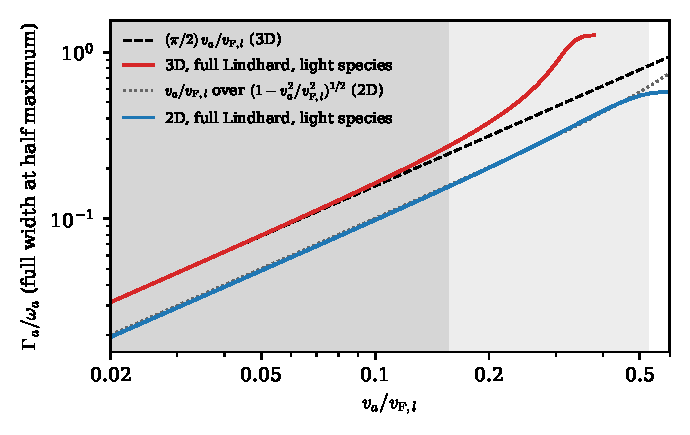
\includegraphics[width=0.82\linewidth]{figures/ch16/limit16_2b.pdf}
\captionof{figure}{Full width at half maximum of the acoustic plasmon over its frequency, against $v_a/v_{\mathrm{F},l}$. Dashed and dotted: \cref{eq:16.2-width} in three and two dimensions. Red and blue: the width of the line in $L = \Imag(-1/\varepsilon)$ with the full frequency dependence of the light carriers' Lindhard function at $q \ll k_{\mathrm{F},l}$. The heavy carriers are cold, and $q = 0.02\,k_{\mathrm{TF},l}$ (3D) and $q_\parallel = 0.02\,q_s$ (2D); the 3D curve stops at $v_a/v_{\mathrm{F},l} = 0.4$, beyond which the line is too broad and asymmetric for a width to be defined. Dark gray: the 3D form within \SI{10}{\percent}, $v_a/v_{\mathrm{F},l} < 0.157$; light gray: the 2D form within \SI{10}{\percent}, $v_a/v_{\mathrm{F},l} < 0.53$. At $v_a/v_{\mathrm{F},l} = 0.02$ the 2D width is \SI{3}{\percent} below its formula because of the finite $q_\parallel/q_s$.}\label{fig:16-demon-limit}
\par}
\smallskip
Beyond the shaded region the light carriers no longer screen statically, the line broadens into their continuum, in three dimensions with a long tail toward high frequency, and the width stops being a small correction to a sharp mode.
\end{limitbox}

\begin{workedexample}{The acoustic plasmon of a two-band sheet}\label{we:16-demon}
Take a sheet suspended in vacuum with two parabolic, spin-degenerate bands of areal density $\nd_{\mathrm{2D}} = \SI{1.0e13}{cm^{-2}}$ each, and masses $m_l = 0.2\,m_e$ and $m_h = 4.0\,m_e$, model values chosen to show the mode. Both bands have $k_{\mathrm{F}} = (2\pi\nd_{\mathrm{2D}})^{1/2} = \SI{156.4}{eV}$ (\SI{0.793}{nm^{-1}}), so $v_{\mathrm{F},l} = 1.53\times10^{-3}$ and $v_{\mathrm{F},h} = 7.65\times10^{-5}$. With $2\mathcal{N}_{\mathrm{F},l} = m_l/\pi$, the screening wavevector is $q_s = e^2m_l/2\pi = 2\alpha m_l = \SI{1.49}{keV}$.

\emph{Velocity.} $v_a^2 = \nd_{\mathrm{2D}}\pi/(m_hm_l) = k_{\mathrm{F}}^2/(2m_hm_l)$, so $v_a = 2.42\times10^{-4}$, or \SI{72.5}{km.s^{-1}}. The mode lies between the continua: $v_a/v_{\mathrm{F},l} = (m_l/2m_h)^{1/2} = 0.158$ and $v_a/v_{\mathrm{F},h} = 3.16$.

\emph{Frequency and width at $q_\parallel = \SI{20}{eV}$.} Here $q_\parallel/k_{\mathrm{F}} = 0.128$ and $q_\parallel/q_s = 0.0134$. The heavy band alone would oscillate at $\omega_{\mathrm{2D},h} = \SI{41.8}{meV}$; screened, $\omega_a = \omega_{\mathrm{2D},h}(1 + q_s/q_\parallel)^{-1/2} = \SI{4.81}{meV}$. \Cref{eq:16.2-width} gives $\varGamma_a/\omega_a = 0.160$, a width of \SI{0.77}{meV}. Both bands together carry the ordinary sheet plasmon at \SI{191.5}{meV} to leading order (\SI{193}{meV} with the $v_{\mathrm{F}}^2$ term of \cref{eq:16.2-2Dpl}), far above $q_\parallel v_{\mathrm{F},l} = \SI{30.6}{meV}$.

\emph{Weight.} By \cref{eq:16.2-share} the line carries $(q_\parallel/(q_\parallel + q_s))^2 = 1.75\times10^{-4}$ of the heavy band's $f$-sum. The light band's own pair continuum carries about as much in the lower half of its range, below $\tfrac12q_\parallel v_{\mathrm{F},l} = \SI{15.3}{meV}$: $1.72\times10^{-4}$ of the same sum, spread over all energies up to there.

\emph{Check.} Now treat both bands with the two-dimensional Lindhard function at $q_\parallel \ll k_{\mathrm{F}}$, so that the heavy band is no longer assumed cold. The peak of $L$ then sits at \SI{4.97}{meV} with a width of \SI{0.76}{meV} ($\varGamma_a/\omega_a = 0.154$), and the first moment within three widths of the peak is $1.76\times10^{-4}$ of the heavy $f$-sum. The heavy band raises the frequency by \SI{3.5}{\percent}, the size of $\tfrac34(v_{\mathrm{F},h}/v_a)^2 = 0.075$ in $\omega_a^2$.

\emph{Kinematics.} A halo particle deposits \SI{4.81}{meV} if $\mchi \ge 2\omega_a/v_{\mathrm{max}}^2 = \SI{1.37}{keV}$, and supplies $q_\parallel = \SI{20}{eV}$ if $2\mchi v_{\mathrm{max}} \ge \SI{20}{eV}$, or $\mchi \ge \SI{3.8}{keV}$. The energy needs a total momentum of only $\omega_a/v_{\mathrm{max}} = \SI{1.8}{eV}$, and the in-plane \SI{20}{eV} decides. The mode, eleven times slower than the fastest halo particles, is reachable by keV-mass dark matter. Its weight, however, is four orders of magnitude below that of the heavy band: a density coupling scatters off this sheet mostly through the pair continuum and the optical plasmon, not through the acoustic one.
\end{workedexample}

\subsection{Layered stacks}\label{sec:16.2-stacks}

A stack of identical sheets with period $a_s$ in a background $\varepsilon_b$, with no tunneling between them, is the simplest layered target. The sheets interact, and \cref{eq:16.2-embed} no longer applies. A density wave $\delta\nd_{\mathrm{2D}}\,\ee^{\ii\vect{q}_\parallel\cdot\vect{r}_\parallel}$ on sheet $n$, with the phase $\ee^{\ii q_zna_s}$ of the external potential, produces $(e^2/2\varepsilon_bq_\parallel)\ee^{-q_\parallel|z - na_s|}$ at height $z$, and the sum over sheets at $z = 0$ is a geometric series. Each sheet therefore sees the kernel
\begin{gather}
  v_{\mathrm{C}}^{\mathrm{L}}(q_\parallel,q_z) = \frac{e^2}{2\varepsilon_bq_\parallel}\sum_n\ee^{-q_\parallel|n|a_s + \ii q_zna_s} = \frac{e^2}{2\varepsilon_bq_\parallel}\,\frac{\sinh q_\parallel a_s}{\cosh q_\parallel a_s - \cos q_za_s} , \notag \\
  S(\vect{q},\omega) = -\frac{2}{a_s}\,\Imag\frac{\tilde R^{\mathrm{2D}}}{1 - v_{\mathrm{C}}^{\mathrm{L}}\tilde R^{\mathrm{2D}}} ,
  \label{eq:16.2-sheets}
\end{gather}
at $T = 0$, per unit volume, for sheets thinner than $1/q$, with the background treated as a static dielectric. For $a_s \to \infty$ the kernel becomes that of an isolated sheet, and $S$ is $1/a_s$ times its structure factor. For $q_\parallel a_s, q_za_s \ll 1$ it becomes $e^2/(\varepsilon_ba_sq^2)$, the bulk kernel acting on the density $\nd_{\mathrm{2D}}/a_s$. In between, the stack carries a band of layer plasmons. For parabolic sheets, $\omega^2 = v_{\mathrm{C}}^{\mathrm{L}}\nd_{\mathrm{2D}}q_\parallel^2/m^*$ runs at small $q_\parallel$ from the bulk plasma frequency of the density $\nd_{\mathrm{2D}}/a_s$ at $q_z = 0$, where all sheets oscillate in phase, down to the acoustic mode $\omega^2 = e^2\nd_{\mathrm{2D}}a_sq_\parallel^2/4\varepsilon_bm^*$ at $q_za_s = \pi$, where neighbors oscillate against each other. The dark-matter momentum along the axis is not reduced to a zone, since the sheets have no structure on the scale of $1/q$; $S$ is periodic in $q_z$ with period $2\pi/a_s$ until the profile of a sheet cuts it off.

Layers many atoms thick respond through their own local dielectric functions. Take layers of materials A and B, of thicknesses $d_A$ and $d_B = a_s - d_A$, filling $f = d_A/a_s$, and local dielectric functions $\varepsilon_A(\omega)$, $\varepsilon_B(\omega)$. When the wavelength is long compared with $a_s$, the field within one period is that of a uniform field across planar boundaries. The tangential field is continuous, so the in-plane displacement is the volume average of $\varepsilon$; the normal displacement is continuous, so the normal field is the volume average of $1/\varepsilon$. The stack is a uniaxial medium with its optic axis along the stacking direction, and with $\theta$ the angle between $\vect{k}$ and that axis,
\begin{gather}
  \varepsilon_\perp = f\varepsilon_A + (1 - f)\,\varepsilon_B , \qquad
  \frac{1}{\varepsilon_\parallel} = \frac{f}{\varepsilon_A} + \frac{1 - f}{\varepsilon_B} , \notag \\
  L(\vect{k},\omega) = \Imag\frac{-1}{\varepsilon_\parallel\cos^2\theta + \varepsilon_\perp\sin^2\theta} \qquad (ka_s \to 0) .
  \label{eq:16.2-emt}
\end{gather}
Since $\varepsilon_\parallel = \varepsilon_A\varepsilon_B/[(1 - f)\varepsilon_A + f\varepsilon_B]$ and $\varepsilon_\perp[(1 - f)\varepsilon_A + f\varepsilon_B] = \varepsilon_A\varepsilon_B + f(1 - f)(\varepsilon_A - \varepsilon_B)^2$, the inverse $1/(\varepsilon_\parallel\cos^2\theta + \varepsilon_\perp\sin^2\theta)$ equals $[(1 - f)\varepsilon_A + f\varepsilon_B]/[\varepsilon_A\varepsilon_B + f(1 - f)(\varepsilon_A - \varepsilon_B)^2\sin^2\theta]$. This is identical, at every filling, to the effective longitudinal response of Lasenby and Prabhu~\cite[Eq.~(16)]{lasenby2022dark}, which they state for $d_A/a_s \ll 1$. The loss function has one line in each direction, at the zero of the denominator. For metal layers in vacuum the line falls toward zero frequency as $\vect{k}$ approaches the axis: with $\varepsilon_A = \varepsilon_\infty(1 - \omega_p^2/\omega^2)$ and small $\theta$ and $f$ it sits at $\omega^2 \simeq f\varepsilon_\infty\omega_p^2\theta^2/\varepsilon_B$, the filling fraction times the plasma frequency squared, reduced by the direction~\cite{lasenby2022dark}.

For $\vect{k}$ in the plane of the layers the response is known in closed form at every $ka_s$. The source $\ee^{\ii kz}$ is uniform across the layers, and the potential is $\psi(x)\ee^{\ii kz}$ with $x$ along the axis. Inside layer $j$ it is the particular solution $1/\varepsilon_jk^2$ plus $C_j\cosh[k(x - x_j)]$, symmetric about the center $x_j$ of the layer. Continuity of $\psi$ and of $\varepsilon\,\partial_x\psi$ at an interface fixes $C_A = (\varepsilon_A - \varepsilon_B)s_B/[k^2\varepsilon_A(\varepsilon_Bs_Bc_A + \varepsilon_As_Ac_B)]$ and $C_B = -\varepsilon_As_AC_A/\varepsilon_Bs_B$, with $s_j = \sinh(kd_j/2)$ and $c_j = \cosh(kd_j/2)$. The average of $k^2\psi$ over a period is the head of $\varepsilon^{-1}$ at the external wavevector:
\begin{keyresult}[Stack of two dielectrics, $\vect{k}$ in the plane]
\begin{equation}
  \frac{1}{\varepsilon(k,\omega)} = \frac{f}{\varepsilon_A} + \frac{1 - f}{\varepsilon_B} - \frac{2}{ka_s}\,\frac{(\varepsilon_A - \varepsilon_B)^2\,s_As_B}{\varepsilon_A\varepsilon_B\,(\varepsilon_As_Ac_B + \varepsilon_Bs_Bc_A)} ,
  \label{eq:16.2-inplane}
\end{equation}
with $L = \Imag[-1/\varepsilon]$, exact for local $\varepsilon_A$, $\varepsilon_B$ at any $ka_s$.
\end{keyresult}
\noindent At $ka_s \to 0$, $s_j \to kd_j/2$, $c_j \to 1$, and the right side becomes $1/\varepsilon_\perp$, the in-plane limit of \cref{eq:16.2-emt}. Expanding to the next order,
\begin{equation}
  \frac{1}{\varepsilon(k,\omega)} = \frac{1}{\varepsilon_\perp} + (ka_s)^2\,\frac{f^2(1 - f)^2(\varepsilon_A - \varepsilon_B)^2}{12\,\varepsilon_\parallel\,\varepsilon_\perp^2} + O\bigl((ka_s)^4\bigr) .
  \label{eq:16.2-corr}
\end{equation}
The correction is quadratic in the period over the wavelength and grows with the contrast between the layers. At $ka_s \to \infty$, $s_j/c_j \to 1$ and the response is the volume average of $1/\varepsilon_j$: each layer then screens as its own bulk. One layer alone follows for $d_B \to \infty$ with $\varepsilon_B = 1$. Multiplied by $a_s$, $\varepsilon^{-1} - 1$ becomes the response per unit area, $d_A(1/\varepsilon_A - 1) - 2(\varepsilon_A - 1)^2s_A/[k\varepsilon_A(\varepsilon_As_A + c_A)]$, and minus this equals the thin-film response of Lasenby and Prabhu up to the real constant $d_A$, which does not enter the loss~\cite[Eq.~(19)]{lasenby2022dark}: the constant is the vacuum term that their response, normalized to $-d/\varepsilon$ for a bulk slab, does not subtract. Its line sits at $\varepsilon_A = -\coth(kd_A/2)$; for a Drude metal at $kd_A \ll 1$ that is $\omega^2 = \omega_p^2kd_A/2$, the sheet plasmon of \cref{eq:16.2-2Dpl} with $\nd_{\mathrm{2D}} = \nd_ed_A$ in vacuum. With $|\varepsilon_A| \gg 1$ and $kd_A \ll 1$ the same expression reduces to the sheet screening of \cref{eq:15.3-sheet}. For a general direction the same matching, with the Bloch condition $\psi(x + a_s) = \ee^{\ii k_xa_s}\psi(x)$ across one period, gives $\varepsilon^{-1}$ by solving four linear equations; it also approaches \cref{eq:16.2-emt} at small $ka_s$.

\begin{limitbox}[Effective medium of a layered stack][lim:16.2c]
For $ka_s \to 0$ a stack of layers with local $\varepsilon_A$, $\varepsilon_B$ and filling $f$ has $1/\varepsilon_L = [(1 - f)\varepsilon_A + f\varepsilon_B]/[\varepsilon_A\varepsilon_B + f(1 - f)(\varepsilon_A - \varepsilon_B)^2\sin^2\theta]$, $\theta$ measured from the stacking axis~\cite[Eq.~(16)]{lasenby2022dark}.
\par\smallskip
{\centering
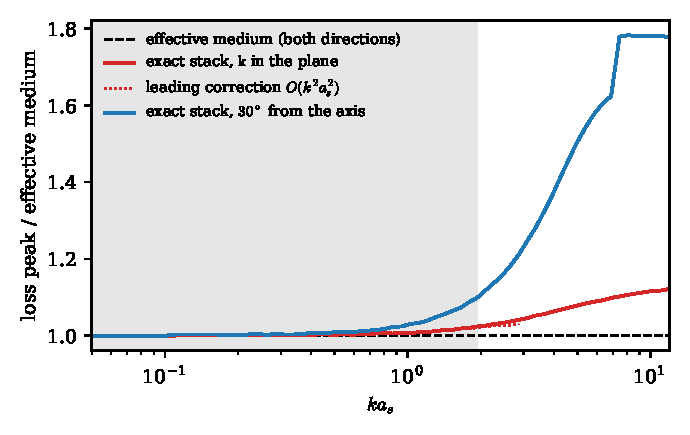
\includegraphics[width=0.82\linewidth]{figures/ch16/limit16_2c.pdf}
\captionof{figure}{Frequency of the loss peak of a model stack relative to the effective medium, against $ka_s$. Layers of \SI{1}{nm} with $\varepsilon_A = 10[1 - \omega_p^2/\omega(\omega + \ii\gamma)]$, $\omega_p = \SI{0.5}{eV}$, $\gamma = 0.1\,\omega_p$, alternate with \SI{4}{nm} of vacuum ($a_s = \SI{5}{nm}$, $f = 0.2$), the toy stack of Lasenby and Prabhu. Red: $\vect{k}$ in the plane, exact (\cref{eq:16.2-inplane}); dotted, the leading correction \cref{eq:16.2-corr}. Blue: $\vect{k}$ at \SI{30}{\degree} from the axis, exact solution of the periodic stack. The effective-medium peaks are at 0.4215 and \SI{0.2740}{eV}. Gray: both within \SI{10}{\percent} of the effective medium, $ka_s < 1.94$. At $ka_s = 12$ the peaks are at 0.473 and \SI{0.487}{eV}, near the surface plasmon of a single layer, $\varepsilon_A = -\varepsilon_B$ (\SI{0.477}{eV} without damping).}\label{fig:16-stack-limit}
\par}
\smallskip
Beyond $ka_s \approx 2$ the field varies within a period, the line of an oblique direction moves up by tens of percent toward that of a single layer, and the stack must be treated layer by layer.
\end{limitbox}

A single undamped line in each direction is the case in which the sum-rule bound of \cref{sec:10.2} can be reached. For $L = A\,\delta(\omega - \omega_{\vect{k}})$ every moment is $K_n = A\omega_{\vect{k}}^n$, and the Hölder inequality behind \cref{eq:10.2-Kn} holds as an equality; the bound \cref{eq:10.2-bound} is then attained when the line sits where $\omega^{-n}\eta$ is largest. A bulk metal places its line at $\omega_p$, far above what light dark matter deposits. A stack moves it down by the filling fraction and the direction, which is why Lasenby and Prabhu proposed it~\cite{lasenby2022dark}. For the model stack of the limit check, \SI{10}{\percent} accuracy at \SI{30}{\degree} ends at $k = \SI{77}{eV}$, the largest momentum transfer, $2\mchi v_{\mathrm{max}}$, of a particle of \SI{14.5}{keV}. Heavier dark matter probes the stack at momenta where the field varies within a period, and needs the full periodic response, with $q_z$ unreduced, that \cref{app:E.21} specifies, and at $k \gtrsim 1/d_A$ also the nonlocal response $\varepsilon_A(\vect{k},\omega)$ of the layer material itself.

\section{Graphene, nanotubes and quantum dots}\label{sec:16.3}

An electron of a graphene sheet that receives more than the work function, about \SI{4.3}{eV}, can leave the sheet without meeting another atom. It then carries into the vacuum the direction and the energy the dark matter gave it, and both can be measured. A bulk crystal turns the same deposit into a cascade of secondary pairs and phonons, and the direction is lost. Carbon nanotubes keep the one-atom thickness and roll the sheet into a cylinder of radius $r_{\mathrm{t}}$. Rolling the sheet quantizes the momentum around the tube and opens a gap in most nanotubes. Quantum dots, nanocrystals a few nanometers across, push confinement to all three directions: a lead sulfide dot \SI{3.3}{nm} across has an optical gap of \SI{1.2}{eV}, against \SI{0.41}{eV} for the bulk crystal, and it re-emits the energy of a pair as a photon~\cite{blanco2023dark}.

\subsection{Electron ejection into vacuum}\label{sec:16.3-ejection}

Take an electron in band $i$ with in-plane crystal momentum $\vect{k}_\parallel$, bound by $E_B(i,\vect{k}_\parallel) \ge 0$ below the Fermi level. It leaves with kinetic energy $E_{\mathrm{ej}} = p_{\mathrm{ej}}^2/2m_e$ when the dark matter deposits
\begin{equation}
  \omega = E_{\mathrm{ej}} + \Phi_{\mathrm{wf}} + E_B(i,\vect{k}_\parallel) ,
  \label{eq:16.3-omega}
\end{equation}
with $\Phi_{\mathrm{wf}}$ the work function, the energy from the Fermi level to the vacuum. For graphene $\Phi_{\mathrm{wf}} \simeq \SI{4.3}{eV}$, and it can be moved by the choice of substrate~\cite[text after Eq.~(5) and footnote~2]{hochberg2017directional}. The largest energy a particle can deposit is its kinetic energy, $\mchi v_{\mathrm{max}}^2/2$, so ejection starts at $\mchi = 2\Phi_{\mathrm{wf}}/v_{\mathrm{max}}^2 = \SI{1.22}{MeV}$, at a momentum transfer of at least $\Phi_{\mathrm{wf}}/v_{\mathrm{max}} = \SI{1.62}{keV}$. This minimum momentum transfer is already a fifth of the momentum scale of a carbon $2p$ orbital, $\beta = Z_{\mathrm{eff}}/2a_0 = \SI{7.51}{keV}$ for the hydrogenic orbital with $Z_{\mathrm{eff}} = 4.03$ that Hochberg et al.\ fit to the overlap of neighboring orbitals~\cite[Eq.~(2)]{hochberg2017directional}. Ejection probes the short-distance structure of the orbitals, as atomic ionization does (\cref{sec:2.2}), and not their tails.

In the independent-particle picture the initial states are the occupied Bloch states $\psi_{i\vect{k}_\parallel}$ of the $\pi$ band and the three $\sigma$ bands, normalized over the sample, and each final state is a hole in the sheet with a free electron. We take the free electron as a plane wave $\ee^{\ii\vect{p}\cdot\vect{r}}/\Vol^{1/2}$ of momentum $\vect{p}$, $|\vect{p}| = p_{\mathrm{ej}}$. Its transition form factor \cref{eq:2.2-ff} is the momentum-space wavefunction of the initial state, $M_{\mathrm{PW}}(\vect{p},\vect{q}) = \tilde\psi_{i\vect{k}_\parallel}(\vect{p} - \vect{q})$, and the structure factor of \cref{eq:4.2-Sab} becomes
\begin{equation}
  S_{\mathrm{ej}}(\vect{q},\omega) = \frac{2\pi}{\Vol}\sum_{i,\vect{k}_\parallel,\sigma}\int\frac{\dd^3p}{(2\pi)^3}\,|M(\vect{p},\vect{q})|^2\,\delta\bigl(\omega - E_{\mathrm{ej}} - \Phi_{\mathrm{wf}} - E_B(i,\vect{k}_\parallel)\bigr) ,
  \label{eq:16.3-Sej}
\end{equation}
with $M = M_{\mathrm{PW}}$ for plane waves and $\sigma$ the spin. Only energy is conserved. Since the bound state is not a momentum eigenstate, it supplies whatever part of $\vect{q}$ the electron does not leave with, and $\vect{p}$ and $\vect{q}$ are independent variables. Inserting \cref{eq:16.3-Sej} and $|\tilde V|^2 = \pi\sigmae\FDM^2/\mu_{\chi e}^2$ (\cref{eq:1.4-Vsq}) into \cref{eq:8.2-spectrum}, with $\rho_T\Vol = N_{\mathrm{cell}}M_{\mathrm{cell}}$, the factors $2\pi\cdot\pi/(2\pi)^3$ combine into $1/4\pi$, and the rate per unit mass is a sum of cross-sections, one for each occupied state:
\begin{equation}
  \begin{gathered}
  \mathcal{R} = \frac{\rho_\chi}{\mchi\,N_{\mathrm{cell}}M_{\mathrm{cell}}}\sum_{i,\vect{k}_\parallel,\sigma}\int\dd^3v\,f_\chi(\vect{v})\,\langle\sigma v\rangle_{i\vect{k}_\parallel}(\vect{v}) ,\\
  \langle\sigma v\rangle_{i\vect{k}_\parallel} = \frac{\sigmae}{\mu_{\chi e}^2}\int\frac{\dd^3p}{(2\pi)^3}\int\frac{\dd^3q}{4\pi}\,\FDM(q)^2\,|M(\vect{p},\vect{q})|^2\,\delta\Bigl(E_{\mathrm{ej}} + \Phi_{\mathrm{wf}} + E_B + \frac{q^2}{2\mchi} - \vect{q}\cdot\vect{v}\Bigr) .
  \end{gathered}
  \label{eq:16.3-rate}
\end{equation}
For plane waves the cross-section is that of Hochberg et al.~\cite[Eq.~(5)]{hochberg2017directional}. They write the sum over states as $2N_{\mathrm{C}}A_{\mathrm{cell}}\int\dd^2k_\parallel/(2\pi)^2$ per band, with $N_{\mathrm{C}}$ the number of carbon atoms per unit mass and $A_{\mathrm{cell}}$ the area of the unit cell. They take for $\tilde\psi$ the tight-binding function of one atom and its three nearest neighbors~\cite[Eqs.~(1), (3), (7)]{hochberg2017directional}. A nanotube changes only the sum over states. Going once around the tube must return the Bloch phase, so the momentum around the circumference takes the values $n/r_{\mathrm{t}}$. Then $A_{\mathrm{cell}}\int\dd^2k_\parallel/(2\pi)^2$ becomes $(A_{\mathrm{cell}}/2\pi r_{\mathrm{t}})\sum_n\int\dd k_z/2\pi$, with $k_z$ along the axis; with this sum over states, \cref{eq:16.3-rate} is the rate of Cavoto et al.~\cite[Eqs.~(16)--(18), (23)]{cavoto2018sub}.

With Bloch states, the in-plane part of $\vect{p} - \vect{q}$ is fixed up to a reciprocal-lattice vector by the crystal momentum of the hole. A Bloch state normalized over $N_{\mathrm{cell}}$ cells has $|\tilde\psi_{i\vect{k}_\parallel}(\vect{k})|^2 \propto \sum_{\vect{G}}\delta^2(\vect{k}_\parallel' - \vect{k}_\parallel - \vect{G})$, with $\vect{k}_\parallel'$ the in-plane part of $\vect{k}$. As a result, each direction of the ejected electron selects one state of each band, with its own binding energy. The selection of one state per band is the origin of the diffraction pattern that Hochberg et al.\ find in the angular distribution of electrons ejected by a cold stream~\cite[Sect.~III]{hochberg2017directional}. The halo washes the pattern out but keeps the forward peak: the momentum-space orbital is largest when $\vect{p} - \vect{q}$ is small, and the electron leaves close to the direction of $\vect{q}$, which follows the dark-matter velocity. For the standard halo they find the forward rate about twice the backward rate between \SI{10}{MeV} and \SI{10}{GeV}~\cite[Sect.~III]{hochberg2017directional}, and the daily rotation of a fixed sheet modulates both rates.

The orbitals and the binding energies are the material input. They come from a density-functional ground state, with maximally localized Wannier functions for the occupied bands and an all-electron orbital for the carbon 1s shell, which a pseudopotential lacks (\cref{app:E.21}).

\paragraph{Orthogonality of the final state.} A plane wave is not an eigenstate of the sheet, and it is not orthogonal to the state the electron leaves. As $q \to 0$, $M_{\mathrm{PW}}$ tends to $\tilde\psi_{i\vect{k}_\parallel}(\vect{p})$, which is not zero, so plane waves predict ejection with no momentum transfer, although $\ee^{\ii\vect{q}\cdot\vect{r}} \to 1$ cannot connect two orthogonal eigenstates. The cure is to orthogonalize the final state to the occupied states, $|\chi_{\vect{p}}\rangle = |\vect{p}\rangle - \sum_n|\psi_n\rangle\langle\psi_n|\vect{p}\rangle$, the orthogonalized plane wave (OPW). Its transition form factor is
\begin{equation}
  M_{\mathrm{OPW}}(\vect{p},\vect{q}) = \tilde\psi_i(\vect{p} - \vect{q}) - \sum_{n\in\mathrm{occ}}\tilde\psi_n(\vect{p})\,f_{i\to n}(\vect{q}) ,
  \label{eq:16.3-opw}
\end{equation}
with $f_{i\to n}$ the form factor \cref{eq:2.2-ff} between occupied states, here written with a single index for $(i,\vect{k}_\parallel)$. Since $f_{i\to n}(\vect{q}) = \delta_{in} + O(q)$, the term without momentum transfer cancels and $M_{\mathrm{OPW}} = O(q)$. To size the orthogonalization correction we take the hydrogenic $2p_z$ orbital above, $\psi \propto r\ee^{-\beta r}\cos\theta$ with $\tilde\psi(\vect{k}) \propto \beta k_z/(\beta^2 + k^2)^3$~\cite[Eq.~(4)]{hochberg2017directional}, orthogonalize the plane wave to it alone, and average over the orientation of the sheet. Integrated over the directions of the ejected electron, $|M_{\mathrm{OPW}}|^2/|M_{\mathrm{PW}}|^2$ runs from 0.46 to 25 at $E_{\mathrm{ej}} = 50$ to \SI{100}{eV} and $q = 5$ to \SI{40}{keV}. The ratio depends on $q$ and on the angle between $\vect{q}$ and the orbital axis, and an orbital of the same form with the more diffuse exponent $1.568/a_0$ of Clementi and Raimondi gives 0.4 to 4.3. At \SI{10}{eV} it reaches 740, but only at $q \gg p_{\mathrm{ej}}$, where the plane-wave amplitude has already fallen as $|\vect{p} - \vect{q}|^{-5}$ and contributes little. The rate weights each $(\vect{p},\vect{q})$ by the halo, so these ratios bound the correction without giving it.

For an orbital averaged over orientations, $|M|^2$ integrated over the directions of $\vect{p}$ depends only on $p_{\mathrm{ej}}$ and $q$. Call this integral $K(p_{\mathrm{ej}},q)$. The velocity integral of \cref{eq:16.3-rate} then reduces with \cref{eq:A.8-eta}, $\int\dd^3q\,g(q)\int\dd^3v\,f_\chi\,\delta(\cdots) = 2\pi\int q\,\dd q\,\eta(\vmin)\,g(q)$, and $p^2\dd p = m_ep_{\mathrm{ej}}\,\dd E_{\mathrm{ej}}$ gives the spectrum per electron
\begin{equation}
  \frac{\dd\langle\sigma v\rangle}{\dd E_{\mathrm{ej}}} = \frac{\sigmae\,m_e\,p_{\mathrm{ej}}}{16\pi^3\mu_{\chi e}^2}\int q\,\dd q\,\eta\bigl(\vmin(q,\omega)\bigr)\,\FDM(q)^2\,K(p_{\mathrm{ej}},q) ,
  \label{eq:16.3-iso}
\end{equation}
with $\vmin = \omega/q + q/2\mchi$ and $\omega$ from \cref{eq:16.3-omega}. Summed over the electrons of a full atomic shell with plane waves, \cref{eq:16.3-iso} times $E_{\mathrm{ej}}$ is \cref{eq:2.2-ion} with \cref{eq:2.2-fion-pw}. \Cref{fig:16-ejection} applies it to the $\pi$ electrons of graphene, one per atom, with the momentum density of the isolated orbital. Their binding energies are those of the nearest-neighbor band, $E_B = t|1 + \ee^{\ii\vect{k}\cdot\vect{a}_1} + \ee^{\ii\vect{k}\cdot\vect{a}_2}|$ with $\vect{a}_{1,2}$ the primitive vectors and hopping $t = \SI{2.8}{eV}$~\cite[text after Eq.~(5)]{castroneto2009electronic}, spread from 0 to \SI{8.4}{eV} with a mean of \SI{4.41}{eV}. At $\sigmae = \SI{e-37}{cm^2}$ and a heavy mediator the $\pi$ electrons alone give \num{6.9e3} events per kg-year at \SI{10}{MeV} with plane waves and \num{1.0e4} with orthogonalized ones; at \SI{100}{MeV}, \num{2.8e3} and \num{5.2e3}. The orthogonalization raises the rate, by factors of 1.44 and 1.84, and moves the peak of the spectrum up in energy. For a light mediator the factors are only 1.14 and 1.19. The light mediator weights the smallest momentum transfers, a few keV, where the orthogonality term lowers the squared amplitude (to 0.46--0.74 of the plane-wave value at $q = \SI{5}{keV}$ for $E_{\mathrm{ej}} = \SI{50}{eV}$) and so partly cancels the gain at larger $q$.

\begin{figure}[tbp]
  \centering
  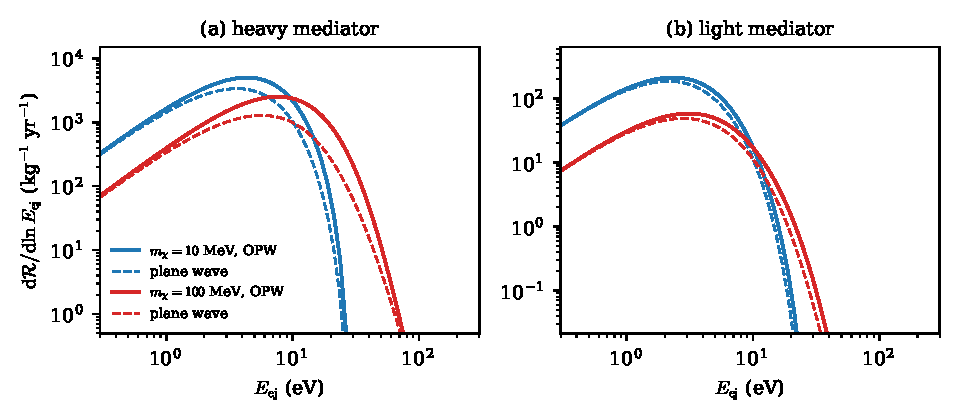
\includegraphics[width=\linewidth]{figures/ch16/fig16_3.pdf}
  \caption{Ejection spectra of the $\pi$ electrons of graphene, $\dd\mathcal{R}/\dd\ln E_{\mathrm{ej}}$ per kg-year at $\sigmae = \SI{e-37}{cm^2}$, against the kinetic energy $E_{\mathrm{ej}}$ of the ejected electron, for $\mchi = \SI{10}{MeV}$ (blue) and \SI{100}{MeV} (red): (a) heavy mediator, $\FDM = 1$; (b) light mediator, $\FDM = (\alpha m_e/q)^2$. Dashed: plane-wave final states; solid: final plane wave orthogonalized to the initial orbital, \cref{eq:16.3-opw}. Model: one hydrogenic $2p_z$ orbital per atom with $Z_{\mathrm{eff}} = 4.03$, Bloch interference between neighbors dropped, binding energies of the nearest-neighbor $\pi$ band ($t = \SI{2.8}{eV}$, 0 to \SI{8.4}{eV}), work function \SI{4.3}{eV}, sheet orientation averaged, standard halo of \cref{tab:1-shm}. The $\sigma$ electrons are not included.}
  \label{fig:16-ejection}
\end{figure}

\begin{limitbox}[Vacuum ejection with plane-wave final states][lim:16.3a]
The ejection rate of a sheet or a tube with plane-wave final states, $M = \tilde\psi_{i\vect{k}_\parallel}(\vect{p} - \vect{q})$ in \cref{eq:16.3-rate}, is the published form~\cites[Eqs.~(5), (7)]{hochberg2017directional}[Eq.~(23)]{cavoto2018sub}.
\par\smallskip
{\centering
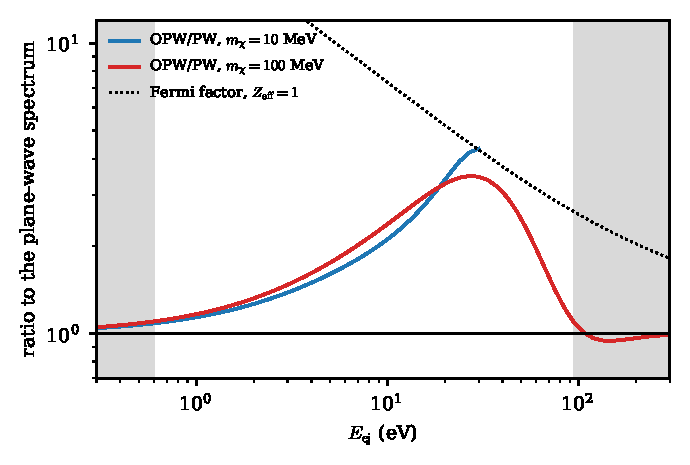
\includegraphics[width=0.85\linewidth]{figures/ch16/limit16_3a.pdf}
\captionof{figure}{Ejection spectrum of graphene $\pi$ electrons with orthogonalized final states, \cref{eq:16.3-opw}, divided by the plane-wave spectrum, against the kinetic energy $E_{\mathrm{ej}}$ of the ejected electron, for $\mchi = \SI{10}{MeV}$ (blue, which ends at \SI{31}{eV}) and \SI{100}{MeV} (red), heavy mediator, in the model of \cref{fig:16-ejection}. Thin line: the plane-wave form. Dotted: the Fermi factor \cref{eq:2.2-fermi} with $Z_{\mathrm{eff}} = 1$, the largest final-state enhancement an unscreened hole can produce. Gray: the orthogonalized spectrum within \SI{10}{\percent} of the plane-wave one, $E_{\mathrm{ej}} < \SI{0.60}{eV}$ and, for \SI{100}{MeV}, $E_{\mathrm{ej}} > \SI{94}{eV}$.}\label{fig:16-limit-ejection}
\par}
\smallskip
Between these energies, where most of the rate lies, orthogonality raises the spectrum by factors up to 3.5 at \SI{100}{MeV} (2.1 at \SI{10}{eV} and 4.3 at the kinematic end for \SI{10}{MeV}), and the attraction of the hole can add up to the Fermi factor, 7.3 at \SI{10}{eV} and 2.6 at \SI{100}{eV}; neither factor is fixed until all occupied orbitals and true scattering states are used.
\end{limitbox}

The second correction to the plane-wave rate is the final-state interaction. The ejected electron leaves a hole behind, and an unscreened point charge would enhance the slow part of the spectrum by the Fermi factor \cref{eq:2.2-fermi}, 7.3, 3.4 and 2.6 at $E_{\mathrm{ej}} = 10$, 50 and \SI{100}{eV}. Graphene screens the hole with its own electrons, and this screening pushes the factor toward one, and the ejected electron travels only atomic distances near the nuclei before it is in vacuum; for these two reasons Hochberg et al.\ leave the factor out~\cite[text after Eq.~(6)]{hochberg2017directional}. A semiconducting tube screens less. The two corrections cannot simply be multiplied: an orthogonalized plane wave is not a scattering state of the hole, and multiplying it by a Fermi factor counts part of the same distortion twice. The consistent final state is a scattering state of the sheet's own potential plus the screened hole.

\subsection{Semiconducting nanotubes}\label{sec:16.3-tubes}

Below the work function a tube responds through pairs within its own bands. Rolling the sheet quantizes the momentum around the circumference in steps of $1/r_{\mathrm{t}}$, and the Dirac cones of graphene are cut along lines. A tube is metallic when a line passes through a Dirac point; otherwise the nearest line misses it by a third of the spacing, and the subbands, labeled $n$, are massive Dirac bands in one dimension with half-gaps $\Delta_n = nv_{\mathrm{D}}/3r_{\mathrm{t}}$ for $n = 1, 2$. With the velocity $v_{\mathrm{D}} = \num{3.02e-3}$ of \cref{sec:16.2}, or \SI{9.1e5}{m.s^{-1}}, a tube \SI{1}{nm} across has $2\Delta_1 = \SI{0.80}{eV}$. The edge is reached through momentum across the tube, which the structure factor \cref{eq:16.2-embed} does not see except through $|F_\perp|^2 = J_0(q_\perp r_{\mathrm{t}})^2$. At the edge $q_\parallel = 0$ and $\omega = 2\Delta_n$, and since $q \ge \omega/v_{\mathrm{max}}$ the dark matter needs $q_\perp \ge 2\Delta_n/v_{\mathrm{max}}$, that is $q_\perp r_{\mathrm{t}} \ge 2nv_{\mathrm{D}}/3v_{\mathrm{max}}$, independent of the radius: 0.76 for the first subband, where $J_0^2 = 0.74$, and 1.52 for the second, where $J_0^2 = 0.25$. For a \SI{1}{nm} tube the first edge opens at $\mchi = 4\Delta_1/v_{\mathrm{max}}^2 = \SI{226}{keV}$.

Each subband pair is $h = v_{\mathrm{D}}k\sigma_x + \Delta_n\sigma_z$, the one-dimensional form of \cref{eq:7.3-H}, with $k$ along the axis and $g_{\mathrm{deg}} = 4$ for spin and valley. The interband response per unit length follows from two symmetries before any integral is done. The model is invariant under Lorentz boosts with $v_{\mathrm{D}}$ in place of the speed of light, and its density is the time component of a conserved current. The response then has the form $q_\parallel^2\,\mathfrak{p}(s)$, with $s = \omega^2 - v_{\mathrm{D}}^2q_\parallel^2$ the invariant of \cref{sec:7.3} and $\mathfrak{p}$ a function of $s$ alone, and it is enough to compute the response at small $q_\parallel$. There the pair is made at $\pm k$ with $\omega = 2\varepsilon_k$, $\varepsilon_k = (v_{\mathrm{D}}^2k^2 + \Delta_n^2)^{1/2}$. The spinors of the two bands are rotated by the angle $\theta_k$ with $\tan\theta_k = v_{\mathrm{D}}k/\Delta_n$, and the interband overlap is $|\langle +,k + q_\parallel|-,k\rangle|^2 = \tfrac14(\partial_k\theta_k)^2q_\parallel^2 = q_\parallel^2v_{\mathrm{D}}^2\Delta_n^2/4\varepsilon_k^4$. Inserting it in $-\Imag\tilde R = (g_{\mathrm{deg}}/2)\int\dd k\,|\langle +|-\rangle|^2\,\delta(\omega - \varepsilon_k - \varepsilon_{k+q_\parallel})$, summing the two roots and replacing $\omega^2$ by $s$,
\begin{equation}
  -\Imag\tilde R^{\mathrm{1D}}_n(q_\parallel,\omega) = \frac{2g_{\mathrm{deg}}v_{\mathrm{D}}q_\parallel^2\Delta_n^2}{s^{3/2}\,(s - 4\Delta_n^2)^{1/2}}\,\Theta(s - 4\Delta_n^2) .
  \label{eq:16.3-R1D}
\end{equation}
The inverse square root at $s = 4\Delta_n^2$ is the van Hove singularity of a one-dimensional band edge. The factor multiplying $q_\parallel^2$ integrates to $g_{\mathrm{deg}}v_{\mathrm{D}}$ over $s$, whatever $\Delta_n$; as $\Delta_n \to 0$ it becomes $g_{\mathrm{deg}}v_{\mathrm{D}}\delta(s)$, the single line of the metallic tube in \cref{sec:16.2}.

In the random-phase approximation the subbands are screened together by the tube kernel \cref{eq:16.2-kernel1D}, $\varepsilon_{\mathrm{1D}} = 1 - v_{\mathrm{C}}^{\mathrm{1D}}\sum_n\tilde R^{\mathrm{1D}}_n$, with the real part of $\tilde R^{\mathrm{1D}}_n$ from \cref{eq:16.3-R1D} by the Kramers--Kronig relation (\cref{app:C.5}), and $S_{\mathrm{1D}} = -2\Imag(\sum_n\tilde R^{\mathrm{1D}}_n/\varepsilon_{\mathrm{1D}})$ at $T = 0$ enters \cref{eq:16.2-embed}. At $q_\parallel r_{\mathrm{t}} \gg 1$ the kernel tends to $\alpha/q_\parallel r_{\mathrm{t}}$, which is the sheet kernel $2\pi\alpha/q_\parallel$ of \cref{eq:16.2-kernel2D} (in vacuum) shared over the circumference $2\pi r_{\mathrm{t}}$: at wavelengths shorter than the radius the tube screens like the flat sheet it was rolled from. Two effects lie outside this response. Transitions between subbands of different $n$ carry angular momentum around the tube and enter through the higher azimuthal harmonics of the transverse form factor. And the electron and the hole of a pair attract each other strongly in one dimension; the attraction binds excitons below each edge, moves the weight of the van Hove singularity into the excitons, and is the Bethe--Salpeter correction of \cref{sec:4.9} and \cref{sec:10.5}.

The same response sets the absorption of a dark photon by an array of aligned tubes. As $q_\parallel \to 0$, $v_{\mathrm{C}}^{\mathrm{1D}}\tilde R^{\mathrm{1D}}_n$ vanishes as $q_\parallel^2\ln(1/q_\parallel r_{\mathrm{t}})$: an isolated tube does not screen a uniform field along its axis. Take a dilute array of $\nd_{\mathrm{u}}$ tubes per unit area and a field along the tubes. \Cref{eq:16.2-embed} and $\varepsilon_2 = (e^2/q^2)(-\Imag R)$ then give
\begin{equation}
  \varepsilon_2^{\parallel}(\omega) = 8\pi\alpha\,g_{\mathrm{deg}}v_{\mathrm{D}}\,\nd_{\mathrm{u}}\sum_n\frac{\Delta_n^2}{\omega^3\,(\omega^2 - 4\Delta_n^2)^{1/2}}\,\Theta(\omega - 2\Delta_n) ,
  \label{eq:16.3-eps2}
\end{equation}
and the rate is \cref{eq:10.7-dp} with $L \simeq \varepsilon_2^{\parallel}$, since $|\varepsilon| \simeq 1$ for a dilute array; a randomly polarized field couples with one third of $\varepsilon_2^{\parallel}$. Dividing by the mass density, which is $\nd_{\mathrm{u}}$ times the mass of a tube per unit length, removes the packing, as it did for scattering.

\subsection{Quantum dots}\label{sec:16.3-dots}

A dot of radius $R$ much larger than the lattice constant has a periodic potential locally and a boundary globally. Its states near the band edges are Bloch functions at the edge, $u_\kappa(\vect{r})$ for the valence or conduction band, times envelopes $\psi_{nlm} = R_{nl}(r)Y_{lm}$ that vanish at the surface~\cite[Eqs.~(2)--(4)]{blanco2023dark}. The radial parts are $R_{nl} \propto j_l(\chi_{nl}r/R)$, with $\chi_{nl}$ the $n$th zero of the spherical Bessel function: this is the effective-mass picture of \cref{sec:3.3} in a hard-walled sphere. The levels are $\chi_{nl}^2/2m^*R^2$ for each carrier, and the gap of the dot,
\begin{equation}
  \Delta E_{\mathrm{QD}} = \Eg + \frac{\pi^2}{2R^2}\Bigl(\frac{1}{m_e^*} + \frac{1}{m_h^*}\Bigr) ,
  \label{eq:16.3-gap}
\end{equation}
exceeds the bulk gap by the confinement energy $E_{\mathrm{conf}}$ of the two lowest envelopes~\cite[Eq.~(5)]{blanco2023dark}. The Coulomb attraction of the pair shifts the dot gap by an amount $\sim\alpha/\varepsilon R$, small when $R$ is below the exciton radius $a_x$ of \cref{sec:4.9}, about \SI{20}{nm} in PbS as quoted by Blanco et al.~\cite{blanco2023dark}. For the dots \SI{3.3}{nm} across that they consider, $\Delta E_{\mathrm{QD}} = \SI{1.2}{eV}$ against $\Eg = \SI{0.41}{eV}$, so $E_{\mathrm{conf}} = \SI{0.79}{eV}$, and the electron and the hole are confined independently.

Dots suspended in a solvent or a glass at volume fraction $\varphi_{\mathrm{QD}} \ll 1$ respond independently, and each transition of a dot is screened by its host. A pair moves an electron from a valence envelope $\psi^h$ to a conduction envelope $\psi^e$, and for $q$ small against the inverse lattice constant the matrix element factorizes into the band-edge form factor of one cell times the envelope overlap $\langle\psi^e|\ee^{\ii\vect{q}\cdot\vect{r}}|\psi^h\rangle$. The overlaps obey a closure rule: summed over all conduction envelopes, $\sum_e|\langle\psi^e|\ee^{\ii\vect{q}\cdot\vect{r}}|\psi^h\rangle|^2 = 1$ for every valence envelope. Confinement therefore redistributes the bulk weight in energy without changing its total. When the levels are dense on the scale of the energy resolution, the sum over pairs becomes the joint density of states of the bulk with the gap moved to $\Delta E_{\mathrm{QD}}$, and $S^{\mathrm{QD}} \to \varphi_{\mathrm{QD}}\,S^{\mathrm{bulk}}(\vect{q},\omega)$ with $\Eg \to \Delta E_{\mathrm{QD}}$, the scissor of \cref{sec:10.1}. Blanco et al.\ use this limit for deposits of 2.5 to \SI{10}{eV}, quoting measurements in which the optical response of PbS dots resembles the bulk above about \SI{2.5}{eV}~\cite[Sect.~III\,A]{blanco2023dark}.

The rate per unit mass of dot material follows from \cref{eq:A.8-rateiso}. Blanco et al.\ define the form factor of a dot as $|f_{\mathrm{QD}}(q,\omega)|^2 = \sum_{f}\sum_{i\in\mathrm{cell}}\delta(\omega - E_f + E_i)\,|\langle f|\ee^{\ii\vect{q}\cdot\vect{r}}|i\rangle|^2$, with the initial states of one cell~\cite[Eq.~(10)]{blanco2023dark}; this form factor has the dimension of an inverse energy. The angle-averaged structure factor is then $\bar S = (2\pi/\Omega)\langle|f_{\mathrm{QD}}|^2\rangle$, with $\Omega$ the cell volume and the average taken over the directions of $\vect{q}$. With $\rho_T\Omega = M_{\mathrm{cell}}$,
\begin{equation}
  \frac{\dd\mathcal{R}}{\dd\ln\omega} = \frac{\omega\,\rho_\chi\,\sigmae}{2\mchi\,M_{\mathrm{cell}}\,\mu_{\chi e}^2}\int q\,\dd q\,\eta\bigl(\vmin(q,\omega)\bigr)\,\FDM(q)^2\,\langle|f_{\mathrm{QD}}(q,\omega)|^2\rangle .
  \label{eq:16.3-qdrate}
\end{equation}
In the bulk limit $2\pi\langle|f_{\mathrm{QD}}|^2\rangle = 4\pi\alpha m_e^2|f_{\mathrm{crys}}|^2/q^3$ by \cref{eq:10.1-fcrys}, and \cref{eq:16.3-qdrate} becomes $\omega$ times the isotropic rate \cref{eq:10.1-rateiso} with the scissored gap, the form their numerical rates use through the bulk code of Ref.~\cite{essig2016direct}.

\begin{limitbox}[Quantum-dot rate and its bulk limit][lim:16.3b]
The scattering rate of quantum dots is \cref{eq:16.3-qdrate} with the bulk crystal form factor and the gap moved to the dot gap, $|f_{\mathrm{crys}}(q,\omega;\Eg \to \Delta E_{\mathrm{QD}})|^2$ of \cref{eq:10.1-fcrys} in \cref{eq:10.1-rateiso}~\cite[Eqs.~(6), (10)--(12)]{blanco2023dark}.
\par\smallskip
{\centering
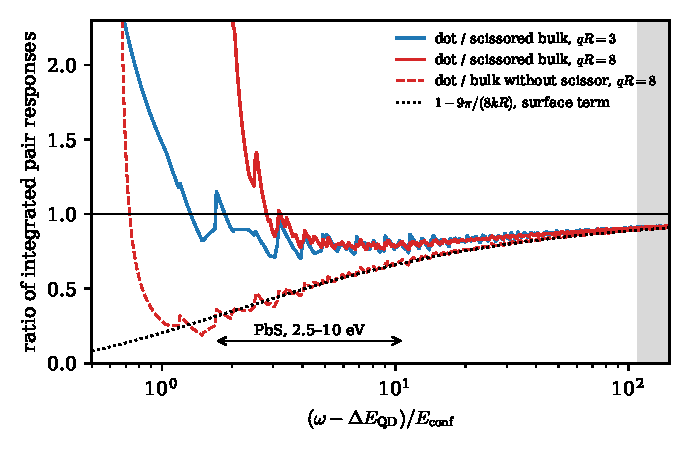
\includegraphics[width=0.85\linewidth]{figures/ch16/limit16_3b.pdf}
\captionof{figure}{Pair response of a hard-walled spherical dot, integrated from its gap up to $\omega$, divided by the same integral of the bulk response with the scissored gap, against $(\omega - \Delta E_{\mathrm{QD}})/E_{\mathrm{conf}}$, for $qR = 3$ (blue) and 8 (red). Model: envelopes of \cref{eq:16.3-gap}, equal electron and hole masses, the band-edge cell factor common to dot and bulk; the direction of $\vect{q}$ averaged. Dashed: the bulk without the scissor at $qR = 8$. Dotted: $1 - 9\pi/(8kR)$, the surface term of the level count of a sphere at $q \to 0$, with $k$ the envelope momentum. Arrow: the range of deposits of PbS dots \SI{3.3}{nm} across, 2.5 to \SI{10}{eV} with $E_{\mathrm{conf}} = \SI{0.79}{eV}$ ($qR \ge 7.5$ there). Gray: the ratios for $qR = 3$ and 8 both within \SI{10}{\percent} of one, above 109 confinement energies ($kR \ge 33$).}\label{fig:16-limit-qd}
\par}
\smallskip
Between 3 and 11 confinement energies above the gap, 3.6 to \SI{10}{eV} for these dots, the hard wall removes states near the surface and the dot carries 0.76 to 1.03 of the scissored bulk response at $qR = 8$ (0.70 to 0.97 at $qR = 3$). The deficit relative to the scissored bulk is set by $kR$ and not by $qR$. Nearer the gap the discrete levels dominate the cumulative ratio, which reaches 2.4 to 66 at $qR = 8$.
\end{limitbox}

The deficit comes from the surface. A wavefunction that must vanish at the surface is depleted within about a wavelength of it, and the number of levels of a sphere below momentum $k$ is $Vk^3/6\pi^2 - Sk^2/16\pi$, with $V$ and $S$ its volume and surface. The second term removes the fraction $9\pi/8kR$ of the bulk count, and the scissor, which shifts the bulk by a fixed energy, corrects only at order $1/(kR)^2$. Between 3 and 11 confinement energies above the gap the model lies 15 to \SI{30}{\percent} below the scissored bulk over most of the range. A real dot has surface atoms and ligands with states of their own, and its wall is not infinitely high. For a real dot the hard wall therefore overstates the depletion, and the measured bulk-like optical response above \SI{2.5}{eV} points to a smaller depletion.

\paragraph{Absorption and the depolarization factor.} A dark photon of mass $m_\phi$ near the dot gap has a reduced wavelength $1/m_\phi v$ of about \SI{0.2}{mm} at \SI{1}{eV}. Over a dot the dark-photon field is uniform, and a dot in a host is a dielectric sphere in a uniform field. Inside, the potential is $-E_{\mathrm{in}}r\cos\theta$; outside it is $-E_0r\cos\theta$ plus a dipole term $\propto\cos\theta/r^2$. Continuity of the potential and of $\varepsilon\,\partial_r\phi$ at $r = R$ gives $E_{\mathrm{in}} = 3\varepsilon_{\mathrm{out}}E_0/(\varepsilon_{\mathrm{in}} + 2\varepsilon_{\mathrm{out}})$, with $\varepsilon_{\mathrm{in}}$ and $\varepsilon_{\mathrm{out}}$ the dielectric functions of the dot and of the host at $\omega = m_\phi$. The polarization of a dilute set of these dielectric spheres gives the Maxwell Garnett dielectric function $\varepsilon_{\mathrm{eff}} = \varepsilon_{\mathrm{out}}[1 + 3\varphi_{\mathrm{QD}}b/(1 - \varphi_{\mathrm{QD}}b)]$, $b = (\varepsilon_{\mathrm{in}} - \varepsilon_{\mathrm{out}})/(\varepsilon_{\mathrm{in}} + 2\varepsilon_{\mathrm{out}})$. To first order in $\varphi_{\mathrm{QD}}$ and for a real $\varepsilon_{\mathrm{out}}$, $\Imag(-1/\varepsilon_{\mathrm{eff}}) = (3\varphi_{\mathrm{QD}}/\varepsilon_{\mathrm{out}})\Imag b = 9\varphi_{\mathrm{QD}}\Imag\varepsilon_{\mathrm{in}}/|\varepsilon_{\mathrm{in}} + 2\varepsilon_{\mathrm{out}}|^2$, the loss function that enters \cref{eq:10.7-dp}. Per unit mass of dot material this loss function replaces the bulk loss function $\Imag\varepsilon_{\mathrm{in}}/|\varepsilon_{\mathrm{in}}|^2$ that a rescaling of the measured photon cross-section with the dot's own $\varepsilon$ uses~\cite[Eq.~(16)]{blanco2023dark}. The two loss functions differ by the depolarization factor
\begin{equation}
  \frac{9\,|\varepsilon_{\mathrm{in}}|^2}{|\varepsilon_{\mathrm{in}} + 2\varepsilon_{\mathrm{out}}|^2} > 1 \iff |\varepsilon_{\mathrm{in}}|^2 > \frac{\varepsilon_{\mathrm{out}}}{2}\,\bigl(\Real\varepsilon_{\mathrm{in}} + \varepsilon_{\mathrm{out}}\bigr) .
  \label{eq:16.3-depol}
\end{equation}
The criterion follows from expanding $|\varepsilon_{\mathrm{in}} + 2\varepsilon_{\mathrm{out}}|^2 = |\varepsilon_{\mathrm{in}}|^2 + 4\varepsilon_{\mathrm{out}}\Real\varepsilon_{\mathrm{in}} + 4\varepsilon_{\mathrm{out}}^2$. The factor tends to 9 when $|\varepsilon_{\mathrm{in}}| \gg \varepsilon_{\mathrm{out}}$, equals one when dot and host are the same medium, and falls below one when $|\varepsilon_{\mathrm{in}}|$ is of order one; for a real $\varepsilon_{\mathrm{in}}$ it exceeds one exactly when $\varepsilon_{\mathrm{in}} > \varepsilon_{\mathrm{out}}$.

\begin{workedexample}{The depolarization factor of a PbS dot in a glass}\label{we:16-depol}
Take a PbS dot in fused silica. Below the bulk gap, at \SI{3.5}{\micro m} (\SI{0.354}{eV}), the dispersion formula of Zemel et al.~\cite{zemel1965electrical} gives $\varepsilon_{\mathrm{in}} = 17.63$, real, and Malitson's fit for silica~\cite{malitson1965interspecimen} gives $\varepsilon_{\mathrm{out}} = 1.977$, both as tabulated in Ref.~\cite{polyanskiy2024refractiveindex}. The field inside the dot is $3\varepsilon_{\mathrm{out}}/(\varepsilon_{\mathrm{in}} + 2\varepsilon_{\mathrm{out}}) = 0.275$ of the field in the glass, against $1/\varepsilon_{\mathrm{in}} = 0.0567$ in bulk PbS, and the depolarization factor is
\begin{equation*}
  \frac{9 \times 17.63^2}{(17.63 + 2\times1.977)^2} = 6.00 .
\end{equation*}
The factor depends little on the exact value of $\varepsilon_{\mathrm{in}}$: $\Real\varepsilon_{\mathrm{in}} = 10$ gives 4.62 and 25 gives 6.71. Wherever $|\varepsilon_{\mathrm{in}}|$ is large, as near the absorption edge of a dot, the bulk formula therefore underestimates the absorption rate by a factor of 4.6 to 6.7. At \SI{5}{eV} silica has $\varepsilon_{\mathrm{out}} = 2.276$. If $\varepsilon_{\mathrm{in}}$ there were $1 + \ii$, an illustrative value near one, the factor would be 0.566, and the bulk formula would overestimate the rate; for $\varepsilon_{\mathrm{in}} = 3 + 3\ii$ it would be 2.45.
\end{workedexample}

Over 2.5 to \SI{10}{eV}, the range of Blanco et al., it is not known whether the depolarization factor is above or below one. The size and even the sign of the depolarization correction need the dielectric function $\varepsilon_{\mathrm{in}}(\omega)$ of real dots of the size used, measured or computed. With it, \cref{eq:16.3-depol} is a one-line evaluation.

\section{Molecular crystals}\label{sec:16.4}

Anthracene, C$_{14}$H$_{10}$, is three benzene rings fused in a row. Its molecules stack in a monoclinic crystal, two to a cell, and the crystal keeps much of the molecule's spectrum: the lowest singlet absorption lies at \SI{3.1}{eV} in the crystal against \SI{3.5}{eV} in the gas~\cite[Tables~I and~III]{rangel2016structural}. A particle must carry $2\times\SI{3.1}{eV}/v_{\mathrm{max}}^2 = \SI{0.883}{MeV}$ to make this excitation (\cref{eq:1.3-mmin}), and an organic crystal turns a large fraction of its singlet excitations into scintillation photons that a photodetector can count, at least 63 percent of them in trans-stilbene~\cite[Sect.~IV\,B]{blanco2021dark}. The electrons that dark matter excites near threshold are in $\pi$ orbitals perpendicular to the flat molecule, and all molecules of the crystal point along two directions, so the rate depends on the angle at which the dark-matter wind meets the molecular planes, and this angle turns with the Earth. The excited electron stays on its molecule, bound to the hole it left: an excitation that stays on one molecule is a \emph{Frenkel exciton}. (The vacancy--interstitial pair of \cref{sec:7.4} is an unrelated object of the same name.)

\subsection{Molecular-basis Bethe--Salpeter equation}\label{sec:16.4-bse}

\Cref{eq:4.9-bse} holds in any basis of electron--hole pairs, and for a molecular crystal the natural one is localized. Combine the occupied Bloch states into orbitals $\phi_{v\mathfrak{o}}$ centered on molecule $\mathfrak{o}$, and the empty ones into orbitals $\phi_{c\mathfrak{o}}$, where $\mathfrak{o} = 1,\dots,N_{\mathrm{mol}}$ labels the molecules of the cell at positions $\vect{r}_{\mathfrak{o}}$ and the cell index is kept implicit. A pair is then an electron in $\phi_{c\mathfrak{o}'}$ and a hole in $\phi_{v\mathfrak{o}}$. If $\mathfrak{o}' = \mathfrak{o}$ the electron stays on the molecule where the hole is; if $\mathfrak{o}' \ne \mathfrak{o}$ the pair is a \emph{charge-transfer} pair, with the electron on a neighbor at a distance $d$.

The kernels of \cref{eq:4.9-kernels} now take a simple form when the orbitals of different molecules do not overlap. The direct kernel contains the overlap densities $\phi_{c\mathfrak{o}'}^*\phi_{c\mathfrak{o}'''}$ and $\phi_{v\mathfrak{o}}^*\phi_{v\mathfrak{o}''}$, which vanish unless the electron and the hole each stay on their molecule. It therefore acts within one molecule, as the intramolecular attraction, and between the partners of a charge-transfer pair, as their screened attraction at distance $d$. The exchange kernel contains the transition densities $\phi_{c\mathfrak{o}'}^*\phi_{v\mathfrak{o}}$, which vanish for a charge-transfer pair; on one molecule they are the charge distribution of a molecular transition, and exchange couples these molecular transitions on different molecules through their Coulomb interaction. In the limit of zero overlap the charge-transfer pairs decouple, and the problem separates into two steps.

The first step is the molecule. Its own block of $H^{\mathrm{exc}}$, with both kernels, gives the singlet excited states $\mathfrak{x}$ of one molecule in the crystal, with energies $E_{\mathfrak{x}}$ and transition densities $\rho^{(\mathfrak{o})}_{0\mathfrak{x}}(\vect{r}) = \langle\mathfrak{x}|\hat{\nd}_e(\vect{r})|0\rangle$. The Fourier transforms of the transition densities are the molecular form factors,
\begin{equation}
  f^{(\mathfrak{o})}_{0\mathfrak{x}}(\vect{q}) = \int\dd^3r\;\ee^{\ii\vect{q}\cdot(\vect{r} - \vect{r}_{\mathfrak{o}})}\,\rho^{(\mathfrak{o})}_{0\mathfrak{x}}(\vect{r}) = \Bigl\langle\mathfrak{x}\Bigl|\sum_j\ee^{\ii\vect{q}\cdot(\vect{r}_j - \vect{r}_{\mathfrak{o}})}\Bigr|0\Bigr\rangle ,
  \label{eq:16.4-ff}
\end{equation}
with the sum over the electrons of the molecule. The singlet factor $\sqrt{g_{\mathrm{deg}}}$ of \cref{sec:10.5} is inside $f$, since $\langle\mathfrak{x}|$ is the full many-electron state. Molecules related by a rotation $\mathsf{R}_{\mathfrak{o}}$ have form factors related by $f^{(\mathfrak{o})}_{0\mathfrak{x}}(\vect{q}) = f_{0\mathfrak{x}}(\mathsf{R}_{\mathfrak{o}}^{-1}\vect{q})$, and at small $q$ each starts as $\ii\vect{q}\cdot\vect{d}_{\mathfrak{x}}$, with $\vect{d}_{\mathfrak{x}} = \langle\mathfrak{x}|\sum_j(\vect{r}_j - \vect{r}_{\mathfrak{o}})|0\rangle$ the transition dipole that fixes the oscillator strength \cref{eq:4.3-osc}.

The second step is the crystal. A molecular excitation on $\mathfrak{o}$ can move to $\mathfrak{o}'$ when its transition density and that of the receiving molecule interact, and the Bloch combinations of crystal momentum $\vect{Q}$ diagonalize the translations. The Frenkel Hamiltonian is
\begin{equation}
  \begin{gathered}
  H^{\mathrm{F}}_{\mathfrak{o}\mathfrak{x},\mathfrak{o}'\mathfrak{x}'}(\vect{Q}) = E_{\mathfrak{x}}\,\delta_{\mathfrak{o}\mathfrak{o}'}\delta_{\mathfrak{x}\mathfrak{x}'} + \mathfrak{J}_{\mathfrak{o}\mathfrak{x},\mathfrak{o}'\mathfrak{x}'}(\vect{Q}) ,\\
  \mathfrak{J}_{\mathfrak{o}\mathfrak{x},\mathfrak{o}'\mathfrak{x}'}(\vect{Q}) = {\sum_{\vect{R}}}'\,\ee^{\ii\vect{Q}\cdot\vect{R}}\int\dd^3r\,\dd^3r'\;\rho^{(\mathfrak{o})}_{0\mathfrak{x}}(\vect{r})^*\,\frac{e^2}{4\pi|\vect{r} - \vect{r}' - \vect{R}|}\,\rho^{(\mathfrak{o}')}_{0\mathfrak{x}'}(\vect{r}') ,
  \end{gathered}
  \label{eq:16.4-HF}
\end{equation}
where the prime drops the term $\vect{R} = 0$, $\mathfrak{o}' = \mathfrak{o}$, since a molecule's interaction with itself is already in $E_{\mathfrak{x}}$. The coupling $\mathfrak{J}$ is the exchange kernel $g_{\mathrm{deg}}K^{\mathrm{x}}$ of \cref{eq:4.9-kernels} between molecules, written in real space; as there, its long-wavelength part, the Fourier component at $\vect{Q}$ itself, is removed and kept in $\varepsilon_{\mathrm{mac}}$. The lattice sum converges only conditionally, and in practice it is done by Ewald's method. The eigenvectors $A^\lambda_{\mathfrak{o}\mathfrak{x}}(\vect{Q})$ and energies $E_\lambda(\vect{Q})$ of $H^{\mathrm{F}}$ are the Frenkel excitons. A molecular level becomes $N_{\mathrm{mol}}$ exciton bands. At $\vect{Q} \to 0$ the exciton bands give the \emph{Davydov splitting} of the absorption line of the molecular level into components, and in a cell with two inequivalent orientations the components absorb light of different polarizations.

The molecular energies and transition densities are the material input. They come from the $GW$ and Bethe--Salpeter equations solved for one molecule in a basis of atom-centered Gaussian orbitals, with singlet energies typically within \SIrange{0.1}{0.3}{eV} of measurement. The crystal enters either as the reaction field of a polarizable medium or through a calculation of the whole periodic crystal (\cref{app:E.6}). In anthracene the environment lowers the fundamental gap, the difference between ionization energy and electron affinity, from \SI{6.9}{eV} in the gas to 3.9--\SI{4.2}{eV} in the crystal~\cite[Tables~I--III]{rangel2016structural}, since the polarization of the neighbors stabilizes a separated electron and hole far more than a neutral excitation. A periodic $GW$ calculation followed by the Bethe--Salpeter equation places the crystal's lowest singlet at \SI{3.3}{eV}, against the measured \SI{3.1}{eV}~\cite[Table~III]{rangel2016structural}.

\subsection{Frenkel-exciton rate}\label{sec:16.4-rate}

The structure factor follows from \cref{eq:4.9-S} with the molecular basis in place of the band pairs. The vertex of the pair $(\mathfrak{o},\mathfrak{x})$ at momentum transfer $\vect{q}$ is $F_{\mathfrak{o}\mathfrak{x}}(\vect{q}) = \ee^{\ii\vect{q}\cdot\vect{r}_{\mathfrak{o}}}f^{(\mathfrak{o})}_{0\mathfrak{x}}(\vect{q})$, where the phase places the molecule in the cell, and the exciton that a momentum transfer $\vect{q}$ creates has crystal momentum $\vect{q}$. Per cell of volume $\Omega$,
\begin{equation}
  S^{\mathrm{F}}(\vect{q},\omega) = \frac{2\pi}{\Omega}\sum_\lambda\frac{\bigl|\sum_{\mathfrak{o}\mathfrak{x}}A^\lambda_{\mathfrak{o}\mathfrak{x}}(\vect{q})^*\,F_{\mathfrak{o}\mathfrak{x}}(\vect{q})\bigr|^2}{|\varepsilon_{\mathrm{mac}}(\vect{q},\omega)|^2}\,\delta\bigl(\omega - E_\lambda(\vect{q})\bigr) .
  \label{eq:16.4-S}
\end{equation}
Each exciton is a coherent superposition of excitations on all molecules, and its weight carries the interference between the molecular excitations through the phases $\ee^{\ii\vect{q}\cdot\vect{r}_{\mathfrak{o}}}$. A detector does not resolve the individual excitons, however. Integrate \cref{eq:16.4-S} over an energy window $\mathcal{B}$ that contains every exciton built from a set of molecular levels and no other, and assume that $\mathfrak{J}$ couples no level of the set to a level outside it and that $\varepsilon_{\mathrm{mac}}$ does not change across the window. Since $H^{\mathrm{F}}$ is Hermitian, as in the Tamm--Dancoff form of \cref{sec:4.9}, the eigenvectors restricted to the set are then complete, $\sum_{\lambda\in\mathcal{B}}A^\lambda(A^\lambda)^\dagger = 1$, and
\begin{equation}
  \int_{\mathcal{B}}\dd\omega\;S^{\mathrm{F}}(\vect{q},\omega) = \frac{2\pi}{\Omega\,|\varepsilon_{\mathrm{mac}}(\vect{q})|^2}\sum_{\mathfrak{o}}\sum_{\mathfrak{x}\in\mathcal{B}}\bigl|f^{(\mathfrak{o})}_{0\mathfrak{x}}(\vect{q})\bigr|^2 .
  \label{eq:16.4-binned}
\end{equation}
The phases have dropped out. Once the structure factor is summed over all Davydov components and over the whole exciton band, the crystal responds as a set of independent molecules, whatever $\mathfrak{J}$ is. At $q \to 0$, where $|f_{0\mathfrak{x}}|^2 \to |\vect{q}\cdot\vect{d}_{\mathfrak{x}}|^2$, \cref{eq:16.4-binned} becomes the oscillator-strength sum rule of molecular-exciton theory: the Davydov components share the dipole strength of the $N_{\mathrm{mol}}$ molecular transitions, $\sum_{\lambda}|\hat{\vect{e}}\cdot\vect{d}_\lambda|^2 = \sum_{\mathfrak{o}}|\hat{\vect{e}}\cdot\vect{d}^{(\mathfrak{o})}_{\mathfrak{x}}|^2$ for every polarization $\hat{\vect{e}}$. The oscillator strengths themselves add up only to order $\mathfrak{J}/E_{\mathfrak{x}}$, since \cref{eq:4.3-osc} weights each component with its own energy. \Cref{eq:16.4-binned} is the same sum rule at every momentum transfer, and \cref{we:16-davydov} works it out for anthracene.

\Cref{eq:16.4-binned} needs the window to hold whole manifolds, $\varepsilon_{\mathrm{mac}}$ and $\eta$ to stay flat across it, and the vertex to be bare. Coupling to a level $\mathfrak{x}'$ outside the window mixes the amplitude $\mathfrak{J}/(E_{\mathfrak{x}} - E_{\mathfrak{x}'})$ of the level $\mathfrak{x}'$ into a state of the window, and the weight of that state changes by
\begin{equation}
  \delta W = \frac{2\Real\bigl[F_{\mathfrak{o}\mathfrak{x}}(\vect{q})^*\,\mathfrak{J}_{\mathfrak{o}\mathfrak{x},\mathfrak{o}'\mathfrak{x}'}(\vect{q})\,F_{\mathfrak{o}'\mathfrak{x}'}(\vect{q})\bigr]}{E_{\mathfrak{x}} - E_{\mathfrak{x}'}} ,
  \label{eq:16.4-borrow}
\end{equation}
which the level outside loses. This intensity borrowing is first order in $\mathfrak{J}/\Delta E$: the cross term of two amplitudes, one of them already small, is as large as the small amplitude itself. The second condition is that $\varepsilon_{\mathrm{mac}}$ and the halo factor $\eta(\vmin)$ stay constant across the window. For a rate the window is set by kinematics: at fixed $q$, $\eta(\vmin)$ changes when $\omega$ changes by about $qv_0$, which is \SI{1.6}{eV} at $q = \SI{2}{keV}$, and much faster near threshold, where $\vmin$ approaches $v_{\mathrm{max}}$. The binned form holds when the exciton bands are narrow on this scale. The third condition is the bare vertex. The literature uses the form factors of the isolated molecule, without $1/|\varepsilon_{\mathrm{mac}}|^2$ and without the local fields that $\mathfrak{J}$ produces at finite $\vect{q}$; both corrections vanish when the dark matter resolves distances shorter than a molecule, $qa_{\mathrm{mol}} \gg 1$, with $a_{\mathrm{mol}}$ the size of the molecule. The static limit of \cref{eq:4.9-eps2} shows why: $\varepsilon_{\mathrm{mac}}(\vect{q},0) - 1 = (2e^2/\Omega q^2)\sum_{\mathfrak{o}\mathfrak{x}}|f^{(\mathfrak{o})}_{0\mathfrak{x}}|^2/E_{\mathfrak{x}}$ is finite at $q \to 0$, where it is the polarizability of the molecules, and falls once the form factors pass their maximum near $q \sim 1/a_{\mathrm{mol}}$.

Insert \cref{eq:16.4-binned} for each molecular level into \cref{eq:8.2-spectrum}, with $\varepsilon_{\mathrm{mac}} = 1$ and the window shrunk to the line at $E_{\mathfrak{x}}$, together with $|\tilde V|^2 = \pi\sigmae\FDM^2/\mu_{\chi e}^2$ (\cref{eq:1.4-Vsq}); integrate over $\omega$; and write the velocity integral at fixed $\vect{q}$ as $\hat f_{\mathrm{gal}}(\vmin + v_{\mathrm{E}}\hat{\vect{q}}\cdot\hat{\vect{v}}_{\mathrm{E}})/q$, with the Radon transform $\hat f_{\mathrm{gal}}$ of \cref{sec:11.7}. The factors $2\pi\cdot\pi/(2\pi)^3$ combine into $1/4\pi$, and with $\rho_T\Omega = M_{\mathrm{cell}}$, the mass of a cell, the rate per unit target mass is
\begin{equation}
  \mathcal{R}(\hat{\vect{v}}_{\mathrm{E}}) = \frac{\rho_\chi\,\sigmae}{\mchi\,\mu_{\chi e}^2\,M_{\mathrm{cell}}}\sum_{\mathfrak{o}\mathfrak{x}}\int\frac{\dd^3q}{4\pi q}\,\FDM(q)^2\,\bigl|f^{(\mathfrak{o})}_{0\mathfrak{x}}(\vect{q})\bigr|^2\,\hat f_{\mathrm{gal}}\bigl(\vmin^{\mathfrak{x}}(q) + v_{\mathrm{E}}\,\hat{\vect{q}}\cdot\hat{\vect{v}}_{\mathrm{E}}\bigr) ,
  \label{eq:16.4-rate}
\end{equation}
with $\vmin^{\mathfrak{x}} = E_{\mathfrak{x}}/q + q/2\mchi$ and $\hat{\vect{v}}_{\mathrm{E}}$ the direction of the Earth's velocity in crystal axes. Averaged over $\hat{\vect{v}}_{\mathrm{E}}$, the angular integral of $\hat f_{\mathrm{gal}}$ gives $2\pi\eta(\vmin)$ (\cref{eq:11.7-ups}), and \cref{eq:16.4-rate} becomes $\rho_\chi\sigmae/(2\mchi\mu_{\chi e}^2M_{\mathrm{cell}})\sum\int q\,\dd q\,\eta\,\FDM^2\langle|f|^2\rangle$. This direction-averaged rate is the rate of Blanco et al.\ for a liquid of aromatic molecules~\cite[Eqs.~(11), (13), (16)--(19)]{blanco2020dark}, with $N_{\mathrm{mol}}/M_{\mathrm{cell}}$ molecules per unit mass and unit detection efficiency. \Cref{eq:16.4-rate} itself is the direction-resolved form they use for the four molecules of trans-stilbene~\cite[Eqs.~(8), (9)]{blanco2021dark}.

\subsection{Davydov splitting in anthracene}\label{sec:16.4-model}

To put numbers on these conditions we use a $\pi$-electron model of anthracene, of the kind the literature uses for benzene and trans-stilbene~\cite{blanco2020dark,blanco2021dark}. The carbon positions are those of the measured crystal structure, with $a = \SI{8.553}{\angstrom}$, $b = \SI{6.016}{\angstrom}$, $c = \SI{11.172}{\angstrom}$ and $\beta = \ang{124.6}$~\cite{brock1990temperature}, and the second molecule of the cell is the image of the first under the twofold screw axis along $b$. We use the crystal axes $a$, $b$ and $c'$, the last perpendicular to $a$ and $b$. The long axes of both molecules make \ang{31} with $c'$, their short in-plane axes make \ang{27} with $b$, and the two molecular planes meet at \ang{51.5}, the herringbone packing of the acenes. The $\pi$ orbitals are combinations of Slater $2p_z$ orbitals with effective charge $Z_{\mathrm{eff}} = 3.15$ on the 14 carbons~\cite[Eq.~(2)]{blanco2020dark}, with the nearest-neighbor resonance integral $-0.63/(m_ex^2)$ at the measured bond length $x$~\cite[Eq.~(A1)]{blanco2021dark}. A self-consistent field of the Pariser--Parr--Pople type refines the $\pi$ orbitals; it adds the repulsion between the $\pi$ electrons to the one-electron (H\"uckel) model. We use a one-center repulsion of \SI{11.13}{eV} and the Mataga--Nishimoto form of the two-center repulsion, a standard parametrization that we take as a model choice. The singlets come from all 49 single excitations of the 14 $\pi$ electrons.

The model places the lowest singlet at \SI{3.85}{eV}, \SI{0.35}{eV} above the measured gas value. For the binned form we shift all levels down by \SI{0.75}{eV}, so that the lowest singlet lies at the measured crystal absorption, \SI{3.1}{eV}, which contains the whole shift from gas to crystal. This state, $L_a$ in Platt's notation, is the transition from the highest occupied to the lowest empty orbital, polarized along the short molecular axis, with $|\vect{d}| = \SI{0.92}{e.\angstrom}$ and a direction-averaged oscillator strength of 0.23. The strong long-axis transition, $B_b$, follows at \SI{4.49}{eV} with an oscillator strength of 2.46. A third state, $L_b$, lies only \SI{18}{meV} above $L_a$ and has no dipole in the model, because of the pairing symmetry of a $\pi$-electron model of an alternant hydrocarbon. With zero differential overlap, the approximation behind the Pariser--Parr--Pople model, each transition density is a sum of atomic $2p_z$ densities weighted by transition charges $\varrho_\mu$ on the carbons, $\sum_\mu \varrho_\mu = 0$, and $f_{0\mathfrak{x}}(\vect{q}) = F_{2p}(\vect{q})\sum_\mu \varrho_\mu\ee^{\ii\vect{q}\cdot\vect{R}_\mu}$, with $\vect{R}_\mu$ the carbon positions relative to the molecular center and $F_{2p}$ the form factor of one $2p_z$ density. Keeping the overlap densities of neighboring orbitals raises the direction-averaged $|f|^2$ of $L_a$ by 1.4 to \SI{11}{\percent} at $q = 2$ to \SI{4}{keV} and gives $L_b$ up to \SI{16}{\percent} of the weight of $L_a$. The coupling $\mathfrak{J}$ of \cref{eq:16.4-HF} is evaluated with the transition charges by Ewald summation. The model is a guide to sizes, not a calculation of anthracene: it has no $\sigma$ electrons, whose polarizability would screen $\mathfrak{J}$, so its couplings are upper estimates.

\begin{workedexample}{The Davydov splitting of anthracene and the binned sum}\label{we:16-davydov}
Take the lowest level, $L_a$, on the two molecules of the cell, in the model above. The twofold screw axis maps the transition dipole $\vect{d}_1$ of the first molecule onto $\vect{d}_2 = \mathsf{R}_b\vect{d}_1$, with $\mathsf{R}_b$ the rotation by \ang{180} about $b$, so that $\vect{d}_1 + \vect{d}_2$ points along $b$ and $\vect{d}_1 - \vect{d}_2$ lies in the $ac$ plane. At $\vect{Q} \to 0$ the Ewald sum of \cref{eq:16.4-HF} gives $\mathfrak{J}_{11} = \mathfrak{J}_{22} = \SI{-196.6}{meV}$, the coupling of each molecule to its translated copies, and $\mathfrak{J}_{12} = \SI{-15.6}{meV}$ between the two orientations. The $2\times2$ Frenkel Hamiltonian has the eigenvalues $E_{L_a} + \mathfrak{J}_{11} \mp |\mathfrak{J}_{12}|$. The measured \SI{3.1}{eV} is the lower of them, so that the shift from gas to crystal is counted once if the molecular level is $E_{L_a} = 3.1 + 0.197 + 0.016 = \SI{3.31}{eV}$:
\begin{equation*}
  E_- = \SI{3.100}{eV}\ (\parallel b) , \qquad E_+ = \SI{3.131}{eV}\ (\perp b) ,
\end{equation*}
a Davydov splitting of $2|\mathfrak{J}_{12}| = \SI{31}{meV}$, with the lower component polarized along $b$. Of the measured lowering from the gas, 3.5 to \SI{3.1}{eV}, the common shift $\mathfrak{J}_{11} = \SI{-0.20}{eV}$ then supplies half, and the polarization of the neighbors, which $\mathfrak{J}$ does not contain, lowers the gas value to $E_{L_a}$. The dipole strengths of the two components are $|\vect{d}_-|^2 = \SI{1.334}{e^2.\angstrom^2}$ and $|\vect{d}_+|^2 = \SI{0.359}{e^2.\angstrom^2}$, and their sum, \SI{1.693}{e^2.\angstrom^2}, equals $2|\vect{d}_1|^2$ exactly, as the sum rule demands. The direction-averaged oscillator strengths add to 0.460 against $2\times0.245 = 0.491$ for two free molecules at $E_{L_a}$; the ratio, 0.938, is close to 0.941, the mean energy of the two components divided by $E_{L_a}$, since each oscillator strength carries its own energy.

The same states at finite momentum transfer show what binning does. At $q = \SI{3}{keV}$ along the short axis of the first molecule, the four excitons built from $L_a$ and $L_b$ carry the weights $|\sum A^*F|^2 = 0.0013$ at \SI{3.299}{eV}, $0.1858$ at \SI{3.356}{eV} and zero in the two $L_b$ states. The two molecules alone carry $|f^{(1)}|^2 = 0.0599$ and $|f^{(2)}|^2 = 0.1272$, since the momentum transfer lies at different angles to them. Coherence concentrates the weight in one exciton, but any window wider than the \SI{58}{meV} between the two lines returns $0.1871$, the incoherent sum. Over the whole zone this band of four states spans 3.04 to \SI{3.40}{eV}, a width of \SI{0.36}{eV}.
\end{workedexample}

\begin{limitbox}[Binned Frenkel rate][lim:16.4a]
The Frenkel-exciton rate binned in $\omega$ is the incoherent sum of molecular form factors at the molecular line energies, \cref{eq:16.4-rate} with \cref{eq:16.4-binned} and $\varepsilon_{\mathrm{mac}} = 1$~\cites[Eqs.~(11), (13), (16)--(19)]{blanco2020dark}[Eqs.~(8), (9)]{blanco2021dark}.
\par\smallskip
{\centering
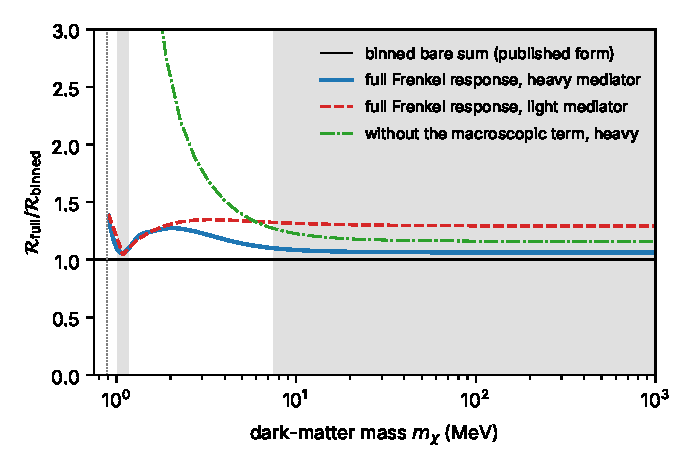
\includegraphics[width=0.85\linewidth]{figures/ch16/limit16_4a.pdf}
\captionof{figure}{Rate of the full Frenkel-exciton response of anthracene divided by the binned rate, against the dark-matter mass, for a heavy (solid) and a light (dashed) mediator, direction-averaged halo. Full response: all 49 $\pi$-electron singlets on both molecules, coupled by $\mathfrak{J}$ and by the macroscopic Coulomb term $(e^2/\Omega q^2)F F^\dagger$, so that no factor $1/|\varepsilon_{\mathrm{mac}}|^2$ is needed (\cref{app:D.12}); the molecular levels are shifted by \SI{0.27}{eV} so that the lowest optically allowed exciton at $\vect{Q} \to 0$ lies at the measured \SI{3.1}{eV} of the binned form. Dash-dotted: the full response without the macroscopic term, heavy mediator. Model of \cref{sec:16.4-model}, $\pi$ electrons only. Gray: the heavy-mediator ratio within \SI{10}{\percent} of one. Dotted: the binned threshold, \SI{0.883}{MeV}.}\label{fig:16-limit-frenkel}
\par}
\smallskip
Just above threshold, between 0.88 and \SI{1.0}{MeV}, the lowest exciton of the full model lies below the binned line and the ratio reaches 1.38. For a heavy mediator between 1.2 and \SI{7.5}{MeV}, and for a light mediator at every mass above \SI{1.2}{MeV}, the mixing of the weak $L_a$ line with the strong $B_b$ transition and the dispersion of the exciton bands change the rate by 10 to \SI{35}{\percent}; the incoherent sum contains neither effect.
\end{limitbox}

Above \SI{30}{MeV} the heavy-mediator rate of the full response in \cref{fig:16-limit-frenkel} exceeds the binned one by \SI{6.3}{\percent}, flat in mass; this excess is the intensity borrowing of \cref{eq:16.4-borrow}. Since $\mathfrak{J}$ is periodic in the crystal momentum, its $L_a$--$B_b$ element keeps the binned weight off by several percent at any momentum transfer. The element is \SI{0.12}{eV} at $\vect{Q} \to 0$ and \SI{0.18}{eV} at a general point of the zone, against an $L_a$--$B_b$ energy difference of \SI{1.4}{eV}. A light mediator weights the momentum transfers near the threshold value $\omega/v_{\mathrm{max}} = \SI{1.17}{keV}$, where $qa_{\mathrm{mol}} \approx 1.6$ for the root-mean-square radius $a_{\mathrm{mol}} = \SI{2.66}{\angstrom}$ of the carbon frame, and there the full rate exceeds the binned one by 29 to \SI{35}{\percent} at all masses above \SI{2}{MeV}. Between 1.2 and \SI{7.5}{MeV} the heavy-mediator ratio reaches 1.27, because the exciton bands spread the levels over tenths of an eV while the halo factor, near threshold, changes on that scale.

The dash-dotted curve shows that the macroscopic term matters most: without it, the local fields alone would raise the rate ninefold at \SI{1.1}{MeV}. The $\pi$ transitions themselves make $\varepsilon_{\mathrm{mac}}(q,0) - 1 = 0.83$ at the threshold momentum and 0.51 at \SI{2}{keV} in the model, so that the factor $1/|\varepsilon_{\mathrm{mac}}|^2$ of \cref{eq:16.4-S} cannot be applied line by line. In the full response the macroscopic term shifts weight up in energy instead of removing it (\cref{sec:4.9}).

\subsection{Charge-transfer excitons and other corrections}\label{sec:16.4-ct}

The zero-overlap limit removes the charge-transfer pairs, and real molecular crystals have some overlap. The simplest description keeps one Frenkel state $|\mathrm{Fr}\rangle$, of energy $E_{\mathrm{Fr}}$, and one charge-transfer state $|\mathrm{CT}\rangle$, of energy $E_{\mathrm{CT}}$, with the electron on a neighbor at distance $d$. The two are coupled by the transfer integral $t_{\mathrm{CT}}$, the sum of the integrals that move the electron and the hole between the molecules. The electron and hole transfer integrals are both proportional to the overlap of the orbitals of the two molecules. Diagonalizing the $2\times2$ problem gives two states $|\pm\rangle$ rotated by the mixing angle $\theta_{\mathrm{CT}}$,
\begin{equation}
  \tan2\theta_{\mathrm{CT}} = \frac{2t_{\mathrm{CT}}}{E_{\mathrm{CT}} - E_{\mathrm{Fr}}} , \qquad
  f_\pm(\vect{q}) = \cos\theta_{\mathrm{CT}}\,f_{\mathrm{Fr}}(\vect{q}) \pm \sin\theta_{\mathrm{CT}}\,f_{\mathrm{CT}}(\vect{q}) ,
  \label{eq:16.4-CT}
\end{equation}
with $f_{\mathrm{CT}}$ the form factor of the charge-transfer state. The transition density of the charge-transfer state is the overlap density of an empty orbital on one molecule and an occupied orbital on the other; it integrates to zero for orthogonal orbitals, so $f_{\mathrm{CT}}(0) = 0$; its dipole is of order $d$ times the overlap, and $|f_{\mathrm{CT}}|^2$ enters at order $q^2d^2$. In the rate the Frenkel line loses the fraction $\sin^2\theta_{\mathrm{CT}}$ of its weight to a new line near $E_{\mathrm{CT}}$, and a binned rate sees this shift of weight up in energy only if the bin ends between the two lines. And $f_{\mathrm{CT}}$ carries the phase difference between two molecules, and the charge-transfer contribution is coherent over distances of order $d$; no Frenkel model contains this coherence. In anthracene the charge-transfer pairs lie near the fundamental gap, 3.9--\SI{4.2}{eV}, some 0.8--\SI{1.1}{eV} above the lowest singlet~\cite[Tables~II and~III]{rangel2016structural}, and for small mixing $\theta_{\mathrm{CT}}^2 \simeq t_{\mathrm{CT}}^2/(E_{\mathrm{CT}} - E_{\mathrm{Fr}})^2$: a transfer integral of \SI{0.1}{eV} would move about one percent of the weight. The mixing grows along the acene series, whose larger members have singlets that extend over several molecules~\cite[Sect.~III\,E]{rangel2016structural}.

The nuclei move when a molecule is excited, and each molecular line becomes a Franck--Condon progression of vibronic replicas with Poisson weights set by a Huang--Rhys factor (\cref{eq:5.6-FC}). In the Condon approximation the progression keeps the total weight of the line, so \cref{eq:16.4-binned} holds for windows that cover it, while the Franck--Condon overlaps narrow the exciton band of each replica. Above the fundamental gap the crystal has a continuum of separated electrons and holes that the Frenkel model lacks, and \cref{eq:16.4-rate} omits it, as the published rates do~\cite{blanco2020dark}; this continuum raises the rate of masses above $2\times\SI{4}{eV}/v_{\mathrm{max}}^2 \approx \SI{1.1}{MeV}$. Triplet excitons cost less, \SI{1.9}{eV} for the lowest triplet of crystalline anthracene~\cite[Table~III]{rangel2016structural}, but a spin-independent density coupling cannot create them, and they enter only through the spin couplings of \cref{sec:10.4}. Finally, the $\pi$-electron model fails at momentum transfers above about \SI{10}{keV}, where the $\sigma$ electrons of the C--C and C--H bonds start to contribute to $|f|^2$. No calculation of the full periodic Bethe--Salpeter response of anthracene at finite $\vect{q}$ exists to compare with the binned molecular sum and with the zero-overlap model.

\subsection{Direction dependence of an anthracene target}\label{sec:16.4-aniso}

A $\pi$ orbital is odd under reflection through the molecular plane, so the transition density between two $\pi$ orbitals is even, and with zero differential overlap it is a sum of atomic densities centered in the plane. For $\vect{q}$ along the normal every phase $\ee^{\ii\vect{q}\cdot\vect{R}_\mu}$ is then the same, and $f = F_{2p}\sum_\mu \varrho_\mu$ vanishes. With the overlap densities kept and the measured, slightly puckered geometry, $|f|^2$ of $L_a$ at $q = \SI{2.07}{keV}$ is $1\times10^{-7}$ along the normal, against $0.25$ along the short axis. The transition density of $L_a$ also changes sign under reflection through the long axis, so that $|f|^2$ along that axis is only $2\times10^{-9}$. Near threshold, where only $L_a$ is reached, the molecule responds to the component of $\vect{q}$ along its short axis alone. In the crystal both short axes lie within \ang{27} of $b$, and the halo makes $\vect{q}$ prefer the direction of the wind when $\vmin$ is close to $v_{\mathrm{max}}$ (\cref{sec:11.7}): the rate is largest when the Earth moves along $b$.

\Cref{fig:16-anthracene} shows the rate of \cref{eq:16.4-rate} in the model, with the 20 singlets below \SI{7.5}{eV}, for the Earth's velocity along each crystal axis. At \SI{10}{MeV} and $\sigmae = \SI{e-37}{cm^2}$ the direction-averaged rate is $8.0\times10^4$ events per kg-year for a heavy mediator and $2.3\times10^4$ for a light one. The heavy-mediator value is comparable to the independent-particle rate of silicon, $1.36\times10^5$ (\cref{sec:10.2}). At \SI{1.0}{MeV}, just above threshold, $L_a$ carries the whole rate, and the largest rate over all directions of the wind, at $\hat{\vect{v}}_{\mathrm{E}} \parallel b$, exceeds the smallest, near the long molecular axes, 92 times for a heavy mediator and 69 times for a light one. The contrast falls quickly with the mass: $L_a$ carries \SI{68}{\percent} of the rate at \SI{2}{MeV} and \SI{19}{\percent} at \SI{10}{MeV}, as $B_b$ and the higher levels fill in the directions $L_a$ cannot use. The ratio of the largest to the smallest rate is 2.3 (heavy) and 5.3 (light) at \SI{1.5}{MeV}, 1.20 and 1.39 at \SI{10}{MeV}, and 1.17 and 1.29 above \SI{100}{MeV}.

\begin{figure}[tbp]
  \centering
  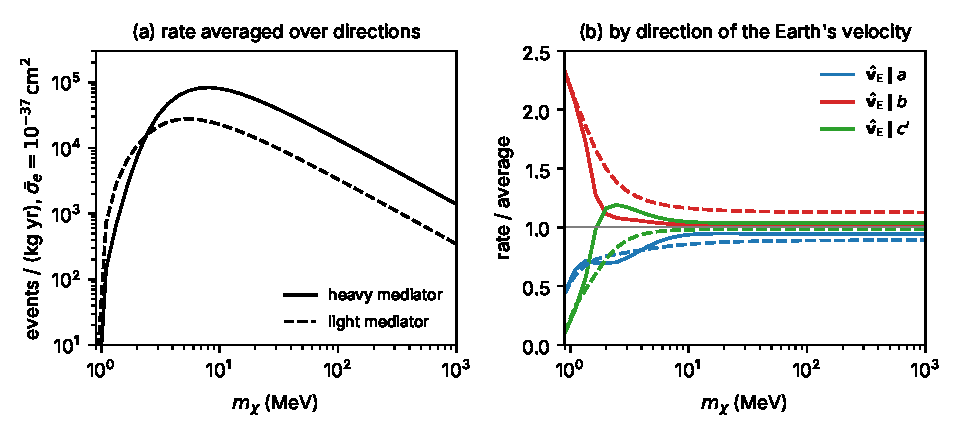
\includegraphics[width=\linewidth]{figures/ch16/fig16_4.pdf}
  \caption{Frenkel-exciton rate of an anthracene crystal in the binned form \cref{eq:16.4-rate}, per kg-year at $\sigmae = \SI{e-37}{cm^2}$, standard halo of \cref{tab:1-shm}. (a) Rate averaged over the directions of the Earth's velocity $\hat{\vect{v}}_{\mathrm{E}}$, heavy (solid) and light (dashed, $\FDM = (\alpha m_e/q)^2$) mediator. (b) Rate for $\hat{\vect{v}}_{\mathrm{E}}$ along the crystal axes $a$, $b$ and $c'$ (perpendicular to $a$ and $b$), divided by the average; heavy (solid) and light (dashed) mediator. The rate is even in $\hat{\vect{v}}_{\mathrm{E}}$. Model of \cref{sec:16.4-model}: $\pi$-electron singlets below \SI{7.5}{eV} of the Pariser--Parr--Pople model on the measured crystal structure, lowest singlet at \SI{3.1}{eV}, form factors with zero differential overlap; the continuum above the fundamental gap is not included.}
  \label{fig:16-anthracene}
\end{figure}

Whatever the mounting and the latitude, $\hat{\vect{v}}_{\mathrm{E}}$ sweeps only part of the sphere in a sidereal day, and the amplitude $A_{\mathrm{day}}$ of \cref{eq:11.7-Aday} cannot exceed $(\mathcal{R}_{\mathrm{max}} - \mathcal{R}_{\mathrm{min}})/(\mathcal{R}_{\mathrm{max}} + \mathcal{R}_{\mathrm{min}})$ over all directions. In the model this bound is 0.98 (heavy) and 0.97 (light) at \SI{1.0}{MeV}, 0.39 and 0.68 at \SI{1.5}{MeV}, 0.09 and 0.17 at \SI{10}{MeV}, and 0.08 and 0.13 at \SI{1}{GeV}. The bound near threshold is a hundred times the daily modulation of silicon, \SI{0.9}{\percent} at \SI{2}{MeV} (\cref{we:11-daily}), because of the crystal class. A cubic crystal has no quadrupole, and its first anisotropic term, the hexadecapole $\ell = 4$, passes the halo only at a few percent; in monoclinic anthracene the quadrupole $\ell = 2$ is allowed and passes at tens of percent of $\mathcal{H}_0$ (\cref{eq:11.7-ups}). Blanco et al.\ reach the same conclusion for trans-stilbene, with a modulation near one at threshold and, at large masses, a modulation above the ten percent of the annual modulation~\cite[Sects.~V, VI]{blanco2021dark}.

\section{Dopants}\label{sec:16.5}

A phosphorus donor in silicon binds its electron by \SI{45.59}{meV}, and dark matter of \SI{13}{keV} can set it free (\cref{we:7-sip}). Compared to the host, the donor has sharp bound lines and a ground state built from six valleys. The $1s(A_1) \to 2p_0$ line at \SI{34.11}{meV} is \SI{4.2}{\micro eV} wide in isotopically purified silicon~\cite[p.~5]{vinh2008silicon}, and a dark photon whose mass falls on it is absorbed several hundred times more strongly than one in the ionization continuum. Between the valley states, dark matter drives transitions that light of the same energy cannot. The drawback is the number of donor electrons, five parts in $10^9$ of the valence electrons at $\nd_{\mathrm{D}} = \SI{e15}{cm^{-3}}$. Du et al.\ proposed doping to \SI{e18}{cm^{-3}} to make up for it~\cite{du2022doped}, at which point the donors begin to merge into an impurity band.

\subsection{Response of dilute donors}\label{sec:16.5-response}

Donors at $\nd_{\mathrm{D}}a^{*3} \ll 1$ act independently, each a hydrogen atom of the crystal (\cref{sec:7.4}). All their transitions lie below the gap of the host, where the host absorbs nothing and its dielectric matrix $\varepsilon_{\mathrm{host}}$ is real. To first order in $\nd_{\mathrm{D}}$ the absorptive part of the response then comes from the donors alone, and the host enters through the screening of the vertex. In \cref{eq:8.4-screened}, split the proper response into its host and donor parts. To first order in the donor part, each vertex acquires the host factor $(\varepsilon_{\mathrm{host}}^{-1})_{\vect{G}\vect{0}}$, and the donor structure factor is
\begin{equation}
  \begin{gathered}
  S^{\mathrm{D}}_{ab}(\vect{q},\omega) = 2\pi\nd_{\mathrm{D}}\sum_f\langle i|\tilde O_a(\vect{q})^\dagger|f\rangle\langle f|\tilde O_b(\vect{q})|i\rangle\,\delta(\omega - E_f + E_i) , \\
  \tilde n_e(\vect{q}) = \sum_{\vect{G}}\bigl(\varepsilon_{\mathrm{host}}^{-1}\bigr)_{\vect{G}\vect{0}}(\vect{q},\omega)\,n_e(\vect{q} + \vect{G}) ,
  \end{gathered}
  \label{eq:16.5-SD}
\end{equation}
for $T \ll E_{\mathrm{b}}^{\mathrm{D}}$, with $|i\rangle$ the donor ground state and $f$ its excited and ionized states. The dark matter's potential at $\vect{q}$ is screened by the host into components at every $\vect{q} + \vect{G}$, and the donor electron feels all of them. An operator with no proper correlation with the charge (a row of the coupling vector of \cref{sec:8.4-couplings}), such as the spin density of a host without spin--orbit coupling, enters unscreened, $\tilde O = O$. Each donor contributes one electron, and the density does not flip its spin, so there is no factor of two for spin. The scattering rate is \cref{eq:8.2-spectrum} with $S = S^{\mathrm{D}}$ and $\rho_T$ the mass density of the host.

The matrix elements follow from the multivalley donor of \cref{app:D.23}, built on the envelope equation of Kohn and Luttinger~\cite{kohn1955theory}. A state $s$ is $\psi_s = \sum_jc^s_jF^s_j(\vect{r})\,\psi_{c\vect{k}_j}(\vect{r})$, with envelopes $F^s_j$ in the six valleys at $\vect{k}_j$ and valley coefficients $c^s_j$. The product of two cell-periodic parts is a lattice sum, $u_{c\vect{k}_{j'}}^*u_{c\vect{k}_j} = \sum_{\vect{G}}\mathcal{U}_{j'j}(\vect{G})\,\ee^{\ii\vect{G}\cdot\vect{r}}$, with $\mathcal{U}_{jj}(\vect{0}) = 1$. Since the envelopes vary slowly over a cell,
\begin{equation}
  \langle s'|\ee^{\ii\vect{q}\cdot\vect{r}}|s\rangle = \sum_{j,j'}c^{s'*}_{j'}c^s_j\sum_{\vect{G}}\mathcal{U}_{j'j}(\vect{G})\int\dd^3r\,F^{s'*}_{j'}F^s_j\,\ee^{\ii(\vect{q} + \vect{k}_j - \vect{k}_{j'} + \vect{G})\cdot\vect{r}} .
  \label{eq:16.5-ff}
\end{equation}
The envelope integral is the Fourier transform of a function a few nanometers across. For the variational envelope of \cref{sec:7.4} it is $[1 + (r_\perp^2p_\perp^2 + r_\parallel^2p_\parallel^2)/4]^{-2}$ at momentum $\vect{p}$, with $p_\parallel$ along the valley axis, and it is negligible once $p \gg 1/r_\perp = \SI{81}{eV}$. Two kinds of term survive. Intravalley terms, $j = j'$ and $\vect{G} = \vect{0}$, carry momentum transfers up to a few hundred eV. Intervalley terms carry $\vect{q} \simeq \vect{k}_{j'} - \vect{k}_j - \vect{G}$, of order keV.

The same structure fixes the field that the envelope feels. In $\tilde n_e$, the component $n_e(\vect{q} + \vect{G})$ has intravalley matrix elements $\mathcal{U}_{jj}(-\vect{G})$ times the envelope integral at $\vect{q}$. For intravalley transitions, $\tilde n_e = \mathfrak{f}^{\mathrm{loc}}_{\mathrm{D}}\,n_e/\varepsilon_{\mathrm{host}}$, with $\varepsilon_{\mathrm{host}} = 1/(\varepsilon_{\mathrm{host}}^{-1})_{\vect{0}\vect{0}}$ the macroscopic dielectric function of \cref{eq:4.4-epsmac} and
\begin{equation}
  \mathfrak{f}^{\mathrm{loc}}_{\mathrm{D}} = 1 + \varepsilon_{\mathrm{host}}\sum_{\vect{G}\ne\vect{0}}\bigl(\varepsilon_{\mathrm{host}}^{-1}\bigr)_{\vect{G}\vect{0}}\,\mathcal{U}_{jj}(-\vect{G}) .
  \label{eq:16.5-floc}
\end{equation}
The donor electron samples the microscopic field with the weight of the conduction-band density $|u_{c\vect{k}_j}|^2$ in each cell. Both factors of the sum are small: the off-diagonal elements of $\varepsilon_{\mathrm{host}}^{-1}$, which produce the local-field corrections of \cref{sec:4.6}, and the Fourier components of a cell-periodic density at $\vect{G} \ne \vect{0}$. In effective-mass theory the ratio is expected to be close to one, since the donor orbit spans many cells and the Lorentz construction of a local cavity field does not apply to it; it has not been computed. Its value for silicon is an open input, which needs the dielectric matrix of the host and the Bloch functions at the minimum, the inputs of \cref{app:E.6}.

\paragraph{Ionization.} For $q$ well below the valley separations, the final state $|\xi\vect{k}\rangle$, a Coulomb envelope $F_{\vect{k}}$ in valley $\xi$, couples to the $A_1$ ground state with amplitude $c_\xi$ times the envelope overlap. Summed over $\xi$, with $\sum_\xi|c_\xi|^2 = 1$, the six valleys give the single-valley result $|\int\dd^3r\,F_{\vect{k}}^*F_{1s}\,\ee^{\ii\vect{q}\cdot\vect{r}}|^2$~\cite[Eq.~(11)]{du2022doped}. For an isotropic hydrogenic envelope of radius $a^* = (2m^*E_{\mathrm{b}}^{\mathrm{D}})^{-1/2}$ this overlap, summed over the directions of $\vect{k}$, is the generalized oscillator strength of the hydrogen $1s$ state. With $L = (e^2/2q^2)S$ at $T = 0$ (\cref{eq:4.4-SL}), the donor part of the loss function is
\begin{equation}
  L^{\mathrm{D}}(\vect{q},\omega) = \frac{2^{10}\pi^2\alpha\,m^*\nd_{\mathrm{D}}a^{*4}}{3\,\varepsilon_{\mathrm{host}}^2}\;
  \frac{(3\tilde q^2 + \tilde k^2 + 1)\exp\bigl[-(2/\tilde k)\arctan\bigl(2\tilde k/(\tilde q^2 - \tilde k^2 + 1)\bigr)\bigr]}{\bigl[(\tilde q + \tilde k)^2 + 1\bigr]^3\bigl[(\tilde q - \tilde k)^2 + 1\bigr]^3\bigl(1 - \ee^{-2\pi/\tilde k}\bigr)} ,
  \label{eq:16.5-gos}
\end{equation}
with $\tilde q = qa^*$, $\tilde k = [2m^*(\omega - E_{\mathrm{b}}^{\mathrm{D}})]^{1/2}a^*$, the arctangent taken in $[0,\pi]$, and $\omega > E_{\mathrm{b}}^{\mathrm{D}}$. At $q \to 0$ the bracket reduces to the dipole continuum of hydrogen in \cref{we:4-trk} with $E_B \to E_{\mathrm{b}}^{\mathrm{D}}$.

\paragraph{Valley-orbit lines.} The $1s$ manifold of phosphorus has its $T_2$ and $E$ states \SI{11.70}{meV} and \SI{13.01}{meV} above the $A_1$ ground state (\cref{sec:7.4}). At optical momentum the transitions vanish in effective-mass theory, because the valley vectors of \cref{eq:D.23-vo} are orthogonal and the intervalley terms need keV momenta. Dark matter reaches both. The $E$ states weight the valleys unequally, and the intravalley sum of \cref{eq:16.5-ff} does not cancel once the envelope integrals differ between valleys. For $\vect{q}$ along [100], two valleys have $\vect{q}$ along their axis and four across it. Summed over the two $E$ states,
\begin{equation}
  \sum_E|\langle E|\ee^{\ii\vect{q}\cdot\vect{r}}|A_1\rangle|^2 = \frac29\Bigl[\Bigl(1 + \frac{r_\parallel^2q^2}{4}\Bigr)^{-2} - \Bigl(1 + \frac{r_\perp^2q^2}{4}\Bigr)^{-2}\Bigr]^2 .
  \label{eq:16.5-E}
\end{equation}
It grows as $q^4$, as a quadrupole transition does, and peaks at 0.022 for $q = \SI{150}{eV}$, which particles from \SI{29}{keV} upward can reach. Along [110] the maximum is 0.0032, and along [111], where all six valleys look alike, the transition vanishes, which makes it a directional signal. These numbers assume one effective-mass envelope common to $A_1$ and $E$; the central-cell contraction of $A_1$ changes their size, but not the zeros along [111] and at $q = 0$. The $T_2$ states pair opposite valleys with opposite signs, and since opposite valleys have identical envelopes their intravalley terms cancel at every $q$. The transition $A_1 \to T_2$ needs the intervalley terms, at $|\vect{q}| = 0.685$, 3.60 and \SI{3.88}{keV} between opposite valleys (the first after an umklapp) and 2.33 and \SI{2.74}{keV} between perpendicular ones, with the minima at $0.85\,(2\pi/a)$. The lightest particle that delivers \SI{11.70}{meV} at \SI{0.685}{keV} has \SI{130}{keV}, and at \SI{2.33}{keV} it has \SI{441}{keV}. The strengths of these lines are set by the coefficients $\mathcal{U}_{j'j}(\vect{G})$, which need the Bloch functions at the minima.

\subsection{Dopant absorption}\label{sec:16.5-absorption}

A dark photon couples to the total charge, and its absorption rate is \cref{eq:10.7-dp} with the loss function of the doped crystal. Silicon has no Born charges, and below its gap the host adds only its two-phonon absorption, which at \SI{50}{meV} gives $\Imag(-1/\varepsilon) = \num{5.4e-6}$ at room temperature and less in a cold crystal (\cref{we:11-iso}). The donor part is the $q \to 0$ limit of $(e^2/2q^2)S^{\mathrm{D}}$ from \cref{eq:16.5-SD}, to first order in $\nd_{\mathrm{D}}$. With $\tilde n_e = n_e/\varepsilon_{\mathrm{host}}$ (taking $\mathfrak{f}^{\mathrm{loc}}_{\mathrm{D}} = 1$) and $\ee^{\ii\vect{q}\cdot\vect{r}} \simeq 1 + \ii\vect{q}\cdot\vect{r}$ between orthogonal states:
\begin{keyresult}[Dark-photon absorption by dilute donors]
\begin{equation}
  \begin{gathered}
  L^{\mathrm{D}}(m_\phi) = \frac{\varepsilon_2^{\mathrm{D}}(m_\phi)}{\varepsilon_{\mathrm{host}}^2} , \qquad
  \mathcal{R} = \zeta^2\,\frac{\rho_\chi}{\rho_T}\,L^{\mathrm{D}}(m_\phi) , \\
  \varepsilon_2^{\mathrm{D}}(\omega) = 4\pi^2\alpha\,\nd_{\mathrm{D}}\sum_f|\langle f|\hat{\vect{e}}\cdot\vect{r}|i\rangle|^2\,\delta(\omega - E_f + E_i) ,
  \end{gathered}
  \label{eq:16.5-abs}
\end{equation}
for $\nd_{\mathrm{D}} \ll \nd_{\mathrm{c}}$ and $|\varepsilon^{\mathrm{D}}| \ll \varepsilon_{\mathrm{host}}$, with $\hat{\vect{e}}$ the polarization of the dark photon and $\varepsilon^{\mathrm{D}}$ the donor part of the dielectric function, whose imaginary part is $\varepsilon_2^{\mathrm{D}}$. In a cubic crystal $L^{\mathrm{D}}$ does not depend on $\hat{\vect{e}}$.
\end{keyresult}
\noindent The host screening appears once, through the vertex $\tilde n_e$, and $\varepsilon_2^{\mathrm{D}}$ is the proper response of the donors, which contains none. The same result follows from writing $\varepsilon = \varepsilon_{\mathrm{host}} + \varepsilon^{\mathrm{D}}$ and expanding $\Imag(-1/\varepsilon)$ to first order in $\varepsilon^{\mathrm{D}}$ with a real $\varepsilon_{\mathrm{host}}$. Per donor, the absorption is that of a hydrogen atom whose matrix elements are those of the envelope, suppressed by $1/\varepsilon_{\mathrm{host}}^2 = 1/130$ at the liquid-helium constant $\varepsilon_{\mathrm{host}} = 11.4$ of \cref{sec:7.4}. In this the dopant differs from the Dirac material of \cref{sec:16.1}, where the background constant sits inside the response of the same electrons.

The $A_1$ ground state has every valley with weight $1/6$, and each valley's $p_0$ states carry the dipole along its axis and its $p_\pm$ states across it. The cubic average of $|\langle f|\hat{\vect{e}}\cdot\vect{r}|i\rangle|^2$ is then $|Z_f|^2/3$ for a $p_0$ line and $2|X_f|^2/3$ for a $p_\pm$ line, where $Z_f$ and $X_f$ are the dipole elements of one valley along and across its axis, with $X_f$ summed over the two $p_\pm$ partners. We obtain them from the numerical solution of \cref{eq:7.4-EMT} that gives \cref{fig:7-donor}, extended to the dipole matrix elements, with the measured line energies. The ground state carries the central-cell potential, a Gaussian well of range 3.2 or \SI{6.3}{\angstrom} in the $s$-like channel, tuned to the measured binding of \SI{45.59}{meV}; the two ranges give line strengths within \SI{2}{\percent} of each other. For the $1s(A_1) \to 2p_0$ line, $|Z|^2/3 = \SI{13.6}{\angstrom^2}$, an oscillator strength $2m_e\omega|Z|^2/3 = 0.12$; the $2p_\pm$ line has 0.52. The lines carry \SI{25}{\percent} of the $f$-sum of the donor electron, $\sum_f2m_e(E_f - E_i)|\langle f|\hat{\vect{e}}\cdot\vect{r}|i\rangle|^2 = m_e(2/m^*_\perp + 1/m^*_\parallel)/3 = 3.85$ (\cref{eq:4.3-TRK} with band masses), and the continuum the rest. \Cref{fig:16-donor-lines} shows the resulting spectrum.

\begin{figure}[tbp]
  \centering
  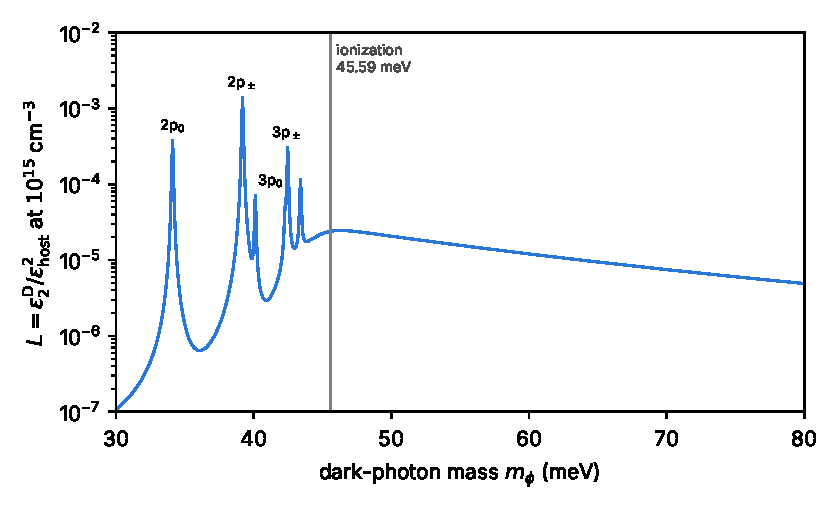
\includegraphics[width=0.85\linewidth]{figures/ch16/fig16_5.pdf}
  \caption{Dark-photon loss function of phosphorus donors in silicon, $L^{\mathrm{D}} = \varepsilon_2^{\mathrm{D}}/\varepsilon_{\mathrm{host}}^2$ of \cref{eq:16.5-abs} at $\nd_{\mathrm{D}} = \SI{e15}{cm^{-3}}$ and $\varepsilon_{\mathrm{host}} = 11.4$, against the dark-photon mass. Anisotropic effective-mass donor (\cref{eq:7.4-EMT}, masses of \cref{tab:3-materials}), solved numerically, with line energies from the measured $1s(A_1)$ at \SI{45.59}{meV} and the measured $2p_0$, $2p_\pm$, $3p_0$ levels. Ground state with a model central cell tuned to \SI{45.59}{meV}. The lines $1s(A_1) \to np_0$, $np_\pm$ ($n = 2$ to 4) are drawn with a display width of \SI{0.1}{meV}; measured widths are tens of times smaller. The continuum and the higher Rydberg lines are smoothed over \SI{1.5}{meV}, comparable to the level spacing of the finite box used for the continuum.}
  \label{fig:16-donor-lines}
\end{figure}

\begin{limitbox}[Dopant absorption][lim:16.5a]
The absorption rate of dark photons on dilute donors is $\mathcal{R} = \zeta^2(\rho_\chi/\rho_T)\,L^{\mathrm{D}}(m_\phi)$, with $L^{\mathrm{D}} = \varepsilon_2^{\mathrm{D}}/\varepsilon_{\mathrm{host}}^2$ the donor loss function of \cref{eq:16.5-abs}~\cite[Eqs.~(10), (12) and the absorption rate after Eq.~(12)]{du2022doped}.
\par\smallskip
{\centering
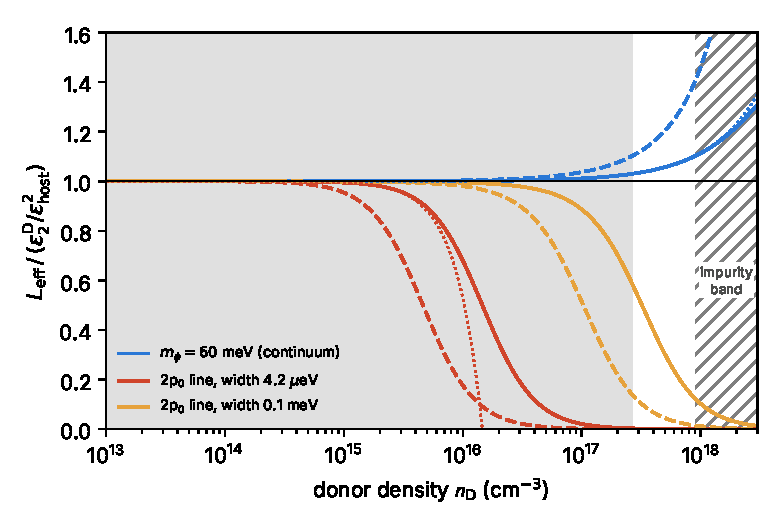
\includegraphics[width=0.85\linewidth]{figures/ch16/limit16_5a.pdf}
\captionof{figure}{Loss function of the effective medium of donors in silicon, $\Imag(-1/\varepsilon_{\mathrm{eff}})$ with $\varepsilon_{\mathrm{eff}} = \varepsilon_{\mathrm{host}}(1 + 2y)/(1 - y)$ and $y = \varepsilon^{\mathrm{D}}/3\varepsilon_{\mathrm{host}}$, divided by the published first-order form $\varepsilon_2^{\mathrm{D}}/\varepsilon_{\mathrm{host}}^2$, against the donor density. Donor model of \cref{fig:16-donor-lines}. Blue: $m_\phi = \SI{60}{meV}$, in the continuum. Red and orange: the $1s(A_1) \to 2p_0$ line center, \SI{34.11}{meV}, for full widths of \SI{4.2}{\micro eV} (narrowest measured) and \SI{0.1}{meV}. Dotted: the expansion $1 - 4\Real y + 4[3(\Real y)^2 - (\Imag y)^2]$. Gray: the continuum ratio within \SI{10}{\percent} of one, $\nd_{\mathrm{D}} < \SI{8.8e17}{cm^{-3}}$. Hatched: $\nd_{\mathrm{D}} > 0.3\,\nd_{\mathrm{c}}$, with $\nd_{\mathrm{c}} \approx \SI{3e18}{cm^{-3}}$, where the donors form an impurity band.}\label{fig:16-limit-dopant}
\par}
\smallskip
Outside the gray region the donors screen the dark photon themselves, and at the narrow line center the first-order form fails already at $\nd_{\mathrm{D}} = \SI{4.8e15}{cm^{-3}}$, where $\varepsilon_2^{\mathrm{D}}$ reaches half of $\varepsilon_{\mathrm{host}}$.
\end{limitbox}

The effective medium is the dilute Clausius--Mossotti form, the Maxwell Garnett function of \cref{sec:16.3} with each donor a polarizable point of polarizability $\alpha_{\mathrm{pol}}(\omega)$ and $\varepsilon^{\mathrm{D}} = \nd_{\mathrm{D}}\alpha_{\mathrm{pol}}$. Its expansion, $L_{\mathrm{eff}} = (\varepsilon_2^{\mathrm{D}}/\varepsilon_{\mathrm{host}}^2)[1 - 4\Real y + O(y^2)]$, shows the two ways the first-order form fails. In the continuum above the lines the donors push $\Real\varepsilon^{\mathrm{D}}$ negative, lower $|\varepsilon_{\mathrm{eff}}|$ and raise the absorption, by \SI{10}{\percent} at \SI{8.8e17}{cm^{-3}}. At the center of a line $\varepsilon^{\mathrm{D}}$ is nearly imaginary, and the ratio becomes $1/[1 + (4/9)(\varepsilon_2^{\mathrm{D}}/\varepsilon_{\mathrm{host}})^2]$: the absorbed field is screened by the donors as the plasmon screens it in \cref{sec:10.7}. A narrow line saturates at a density proportional to its width.

\begin{workedexample}{The $2p_0$ line of Si:P for a dark photon at resonance}\label{we:16-sip-line}
Take $\nd_{\mathrm{D}} = \SI{e15}{cm^{-3}}$ and a dark photon of mass $m_\phi = \SI{34.11}{meV}$, the binding of $1s(A_1)$, \SI{45.59}{meV}, minus that of $2p_0$, \SI{11.48}{meV}. With the line strength $|Z|^2/3 = \SI{13.6}{\angstrom^2}$, the line integral of \cref{eq:16.5-abs} is
\begin{equation*}
  \int\varepsilon_2^{\mathrm{D}}\,\dd\omega = 4\pi^2\alpha\,\nd_{\mathrm{D}}\,\frac{|Z|^2}{3} = \SI{7.73e-6}{eV} .
\end{equation*}
The narrowest measured full width of the line, in isotopically purified silicon, is $\varGamma_{\mathrm{line}} = \SI{0.034}{cm^{-1}} = \SI{4.22}{\micro eV}$, close to the lifetime width $1/T_1 = \SI{3.2}{\micro eV}$ of the $2p_0$ state, which decays by phonon emission in $T_1 = \SI{205}{ps}$~\cite[p.~5]{vinh2008silicon}. For a Lorentzian line the peak is $2/\pi\varGamma_{\mathrm{line}}$ times the integral, $\varepsilon_2^{\mathrm{D}} = 1.17$, and
\begin{equation*}
  L^{\mathrm{D}} = \frac{1.17}{11.4^2} = \num{8.99e-3} ,
\end{equation*}
which the effective medium lowers by half a percent, to \num{8.94e-3}. The dark photon's own spread in energy, $m_\phi v^2/2 \approx \SI{0.017}{\micro eV}$, lies well inside the line. With $\rho_\chi/\rho_T = \SI{0.3}{GeV.cm^{-3}}/\SI{2.33}{g.cm^{-3}}$, the rate is
\begin{equation*}
  \mathcal{R} = \zeta^2\,\frac{\rho_\chi}{\rho_T}\,L^{\mathrm{D}} = \num{5.5e31}\,\zeta^2\ \text{per kg-year} ,
\end{equation*}
and three events per kg-year need $\zeta = \num{2.3e-16}$. In the continuum at \SI{50}{meV} the same crystal has $L^{\mathrm{D}} = \num{2.1e-5}$ and needs $\zeta = \num{4.9e-15}$, twenty times more. The gain holds over a window of masses as wide as the line, $\varGamma_{\mathrm{line}}/m_\phi = \num{1.2e-4}$, and the peak, proportional to $\nd_{\mathrm{D}}/\varGamma_{\mathrm{line}}$, grows with the donor density only while the line keeps its width.
\end{workedexample}

\subsection{The impurity band}\label{sec:16.5-band}

Uncompensated Si:P becomes a metal at low temperature above a donor density $\nd_{\mathrm{c}} \approx \SI{3e18}{cm^{-3}}$, as quoted by Du et al.~\cite[Sect.~II]{du2022doped}. This is the \emph{Mott critical density}, the donor density of the metal--insulator transition named in \cref{sec:7.4}. Their projections use $\nd_{\mathrm{D}} = \SI{e18}{cm^{-3}}$, and their comparison with optical data \SI{1.8e18}{cm^{-3}}, so $\nd_{\mathrm{D}}/\nd_{\mathrm{c}} \approx 0.3$ to 0.6. At these densities the donors are not isolated. Donors sit at random positions, and the probability that a given donor has a neighbor within a distance $d$ is $1 - \exp(-4\pi\nd_{\mathrm{D}}d^3/3)$. For $d$ equal to the orbit diameter, $2r_\perp = \SI{4.86}{nm}$, this is \num{4.8e-4} at \SI{e15}{cm^{-3}}, but 0.38 at \SI{e18}{cm^{-3}} and 0.58 at \SI{1.8e18}{cm^{-3}}. The electron of such a pair hops between the two cores. The hopping splits the $1s$ level of the pair into bonding and antibonding states, shifts its lines, and over a random ensemble spreads the discrete spectrum into a band of states, the \emph{impurity band}. Optical spectra at these densities show it: the lines broaden and the gap below the first line closes~\cite[Sect.~VII.6]{du2022doped}.

The effective medium of \cref{lim:16.5a} shows the same failure from the other side. The static polarizability of an isolated donor, from the numerical solution, is $\alpha_{\mathrm{pol}}(0)/\varepsilon_{\mathrm{host}} = 4\pi\times\SI{1.1e-20}{cm^3}$. At \SI{e18}{cm^{-3}} it raises the static dielectric function of the crystal by a factor of 1.15, and at \SI{1.8e18}{cm^{-3}} by 1.28. The Clausius--Mossotti form diverges at $\nd_{\mathrm{D}}\alpha_{\mathrm{pol}}(0) = 3\varepsilon_{\mathrm{host}}$, at \SI{2.1e19}{cm^{-3}}, above the measured $\nd_{\mathrm{c}}$. The transition, however, comes first from pairs and clusters, whose polarizability and overlap exceed those of isolated donors, and the response of isolated donors, in a dilute medium or an effective one, is wrong at order one near the ionization edge for $\nd_{\mathrm{D}}/\nd_{\mathrm{c}} \approx 0.5$.

What replaces it is the disorder average $\langle S^{\mathrm{D}}(\vect{q},\omega)\rangle$ of a random ensemble of donors, each with its six-valley orbitals and central cell. The hopping between two donors oscillates with their separation, because the valley phases $\ee^{\ii\vect{k}_j\cdot\vect{r}}$ interfere, so a single-valley envelope gets it wrong. The optical data that Du et al.\ use at \SI{1.8e18}{cm^{-3}} contain the impurity band at $q = 0$; how it reshapes $S^{\mathrm{D}}$ at the momenta of scattering, and the absorption near the edge, is the open problem of this section.

\subsection{Donors as final states}\label{sec:16.5-final}

A donor excitation is useful when the deposit could have made nothing else, when the detector can count it before it is lost, and when the donors are dilute. The first condition is kinematic. Between \SI{13}{keV} and the \SI{0.333}{MeV} of the silicon gap (\cref{sec:1.3}), the donor is the only electronic excitation of the crystal that dark matter can reach. Above that it adds a valley structure that the host lacks. The $A_1 \to E$ line of \cref{eq:16.5-E} makes the rate depend on the direction of $\vect{q}$ relative to the crystal axes, and the daily rotation of the laboratory turns this into a modulation.

The second condition depends on the final state. An ionized donor leaves an electron in the conduction band, which a field can collect and a charge-coupled device can count one at a time; this is the readout that Du et al.\ propose~\cite[Sect.~VII.1]{du2022doped}. The donors then must stay neutral without the dark matter. Thermal ionization grows as $\ee^{-E_{\mathrm{b}}^{\mathrm{D}}/T}$, and from the measured capture coefficient of electrons on ionized phosphorus Du et al.\ estimate that at \SI{e18}{cm^{-3}} a temperature of about \SI{5}{K} keeps it below one electron per kg-year. The bias that collects the electron also drives hopping conduction through the impurity band, which a layer of undoped silicon between the doped volume and the readout blocks, as in the blocked-impurity-band infrared detectors~\cite[Sect.~VII.1]{du2022doped}. A bound excitation, such as $2p_0$, has no charge to collect. It returns to the ground state by emitting phonons, within \SI{205}{ps} for $2p_0$~\cite[p.~5]{vinh2008silicon}, and the energy is then a few phonons of at most \SI{34}{meV}. In a doped crystal phonons above \SI{11.70}{meV} can drive the $1s(A_1) \to 1s(T_2)$ and $1s(E)$ transitions of other donors, and only those below are expected to travel ballistically to a sensor~\cite[Sect.~VII.6]{du2022doped}. A bound excitation therefore needs a sensor of single phonons of about \SI{10}{meV}, which no present detector provides, while ionization needs a single-electron counter, which exists. Both need the third condition, $\nd_{\mathrm{D}} \ll \nd_{\mathrm{c}}$, with the bound set by the impurity band of \cref{sec:16.5-band}.

\section{Color centers and broken bonds}\label{sec:16.6}

A fluorine atom knocked off its site in lithium fluoride leaves an anion vacancy, and an anion vacancy that binds an electron is an F center, which absorbs light near \SI{5.1}{eV}~\cite{guerreroperez2025first}. A dark-matter particle of \SI{0.5}{GeV} can give a fluorine nucleus at most \SI{188}{eV} (\cref{eq:1.3-ERmax}), a few times the tens of eV that a displacement costs. A molecule struck on one of its atoms comes apart in the same way when the kick exceeds its bond energy, \SI{4.75}{eV} for H$_2$. The F center and the broken molecule both persist, both lie in a crystal transparent to the light that reads them, and both can be counted singly. Budnik, Cheshnovsky, Slone and Volansky proposed color centers as a target for sub-GeV dark matter~\cite{budnik2018direct}, and Essig, Mardon, Slone and Volansky the breaking of chemical bonds~\cite{essig2017detection}.

\subsection{The color-center creation rate}\label{sec:16.6-cc}

A color center forms after the prompt window of \cref{sec:8.7}. Within that window, a femtosecond after the kick, the struck nucleus moves with the momentum it received and its neighbors have not yet responded; the class $\Lambda$ is a recoil of species $\kappa$ with energy deposit $\omega$ along $\hat{\vect{q}}$. The defect forms during the collision cascade that follows, within picoseconds, and its fate is decided later still, when the close pair recombines or does not and when the vacancy captures an electron or does not. The rate of creating readable centers is therefore the hand-off formula \cref{eq:8.7-handoff} with the cascade distribution $P_{\mathrm{casc}}(N_{\mathrm{eh}}|\Lambda)$ replaced by the probability $Y_{\mathrm{CC}}(\Lambda)$ that a seed of class $\Lambda$ ends as a center that the readout registers. \Cref{sec:18.3} makes precise how a recoil seeds the cascade, and \cref{sec:19.4} treats the energy that defects store. The conditions of \cref{sec:8.7} apply directly: the yield depends on the direction of the recoil relative to the crystal axes, so $\hat{\vect{q}}$ must stay inside the class sum, and a rate averaged over directions before the yield is applied is wrong near threshold.

The yield is a product of four probabilities, each fixed at a different stage:
\begin{equation}
  Y_{\mathrm{CC}}(E_R,\hat{\vect{r}}_R) = p_{\mathrm{FP}}(E_R,\hat{\vect{r}}_R)\;p_{\mathrm{surv}}\;p_q\;f_{\mathrm{opt}} .
  \label{eq:16.6-yield}
\end{equation}
The first, $p_{\mathrm{FP}}$, is the probability that a nucleus set moving with kinetic energy $E_R$ along $\hat{\vect{r}}_R$ leaves a Frenkel pair once the collision has died out. Its lowest crossing is the displacement threshold $E_{\mathrm{d}}(\hat{\vect{r}}_R)$ of \cref{eq:7.4-Ed}, and molecular dynamics computes the threshold direction by direction (\cref{app:E.11}). For an F center the displaced atom must be an anion, either struck directly or hit by a struck cation. The second, $p_{\mathrm{surv}}$, is the probability that the close pair survives recombination over the time between the event and the readout. At millikelvin temperatures thermal hopping is frozen (\cref{sec:7.4}), and only tunneling recombination and the phonons of later events act. The third, $p_q$, is the probability that the vacancy ends in the charge state of the readable center: an F center is a vacancy with one electron, while an empty anion vacancy absorbs elsewhere. The fourth, $f_{\mathrm{opt}}$, is the probability that the readout registers a center that is present. None of the four probabilities enters the response; they are properties of the final state, and the truncation label of \cref{sec:8.5} applies only to the seed.

The seed is an impulsive recoil. Displacement needs $E_R$ of 10 to \SI{60}{eV}, three orders of magnitude above the phonon energies, so the recoil parameter $x_R = E_R/\langle\omega\rangle$ is several hundred and the nuclear response is the Gaussian \cref{eq:11.4-IAgauss} of \cref{sec:11.4}. The momentum transfer, near \SI{1}{MeV} for a fluorine recoil of \SI{27}{eV}, is far above the zone scale. Above the zone scale the coherence corrections of the multiphonon response are already below \SI{10}{\percent} at \SI{18}{keV} in silicon and keep falling (\cref{sec:11.3}). Only the self response of each species remains. For a heavy mediator we insert that response and the yield into \cref{eq:8.7-handoff}, average over orientations as in \cref{sec:11.4}, and count one nucleus of species $\kappa$ per cell of mass $M_{\mathrm{cell}}$. The rate per unit target mass is
\begin{equation}
  \begin{split}
  \mathcal{R}_{\mathrm{CC}} &= \sum_\kappa\frac{M_\kappa}{M_{\mathrm{cell}}}\,\frac{\rho_\chi\,\sigma_{N,\kappa}}{2\mchi\,\mu_{\chi\kappa}^2}\int\dd E_R\int\dd\omega\;\frac{\ee^{-(\omega - E_R)^2/2\sigma_\omega^2}}{(2\pi\sigma_\omega^2)^{1/2}} \\
  &\qquad\times\eta\Bigl(\frac{\omega}{q} + \frac{q}{2\mchi}\Bigr)\,\bigl\langle Y_{\mathrm{CC},\kappa}(\omega,\hat{\vect{r}}_R)\bigr\rangle_{\hat{\vect{r}}_R} ,
  \end{split}
  \label{eq:16.6-ccrate}
\end{equation}
with $q = (2M_\kappa E_R)^{1/2}$, $\sigma_\omega^2 = E_R\langle\omega\rangle_\kappa$ at $T = 0$, $\langle\omega\rangle_\kappa$ the mean phonon energy of the site, $\sigma_{N,\kappa}$ the nuclear cross-section of \cref{eq:2.2-nucleus} with $F_N = 1$, and $\mu_{\chi\kappa}$ the reduced mass with nucleus $\kappa$. In the impulse response the deposit $\omega$ equals the change of kinetic energy of the nucleus, so the yield is evaluated at $\omega$; the initial kinetic energy of the nucleus, $3\langle\omega\rangle_\kappa/4$, is a few hundredths of an eV and is dropped. The direction average of $Y$ is exact only when the recoil directions are isotropic in the crystal frame. For a crystal fixed to the rotating Earth they are not, and the full form keeps $\hat{\vect{r}}_R = \hat{\vect{q}}$ inside the velocity integral; this dependence on the direction of $\vect{q}$ is the origin of the daily modulation of the rate~\cite[Eq.~(10)]{budnik2018direct}.

\Cref{eq:16.6-ccrate} reduces to the published rate in two steps. As $\sigma_\omega \to 0$ the Gaussian becomes $\delta(\omega - E_R)$ and the minimum velocity becomes $q/2\mu_{\chi\kappa}$; the rate is then the free recoil \cref{eq:11.4-LS} per species. Setting then $p_{\mathrm{surv}} = p_q = f_{\mathrm{opt}} = 1$ and $p_{\mathrm{FP}} = \Theta(E_R - E_{\mathrm{d}}(\hat{\vect{r}}_R))$ gives the rate of Budnik et al.~\cite[Eqs.~(1), (5), (7)]{budnik2018direct}. They write it as an integral over $q^2$ with the step $\Theta(q - q_{\min}(\hat{\vect{q}}))$, $q_{\min}^2 = 2M_\kappa E_{\mathrm{d}}$, and with a per-nucleon cross-section and the coherence factor $[f_PZ + f_N(A - Z)]^2$. For equal couplings to protons and neutrons that factor is $A^2$. Their per-nucleon cross-section is the $\sigma_p$ of \cref{eq:2.2-nucleus}, and $\sigma_p$ times $A^2/\mu_{\chi p}^2$ is $\sigma_{N,\kappa}/\mu_{\chi\kappa}^2$. For the threshold surface they take $q_{\min}(\hat{\vect{q}}) = (2M_\kappa\Delta E_B)^{1/2}[1 + a\sin(4\theta)\cos(4\varphi)]$ in crystal axes, with a mean binding energy $\Delta E_B$ and $a = 0.4$~\cite[Eq.~(2) and Table~I]{budnik2018direct}. Their formula counts a dislocated nucleus, not a particular defect, and assumes that the vacancy fills with an electron at once.

The Doppler width is the first correction, and it is small. For a fluorine nucleus in LiF the optical phonons lie between 33.5 and \SI{77.2}{meV}~\cite[Table~I]{griffin2020multichannel}, and we take these two values as the range of $\langle\omega\rangle_{\mathrm{F}}$; at $E_R = \SI{27}{eV}$ the width is 0.95 to \SI{1.44}{eV}, 3.5 to \SI{5.4}{\percent} of the threshold. The zero-point momentum of the nucleus along $\hat{\vect{q}}$, $(M_{\mathrm{F}}\langle\omega\rangle_{\mathrm{F}}/2)^{1/2}$, is 17 to \SI{26}{keV}, against $q_{\min} = \SI{978}{keV}$, a ratio of 0.018 to 0.027, so the classical treatment stands. \Cref{lim:16.6a} shows where the width matters: only where the largest recoil energy is less than 1.22 to 1.36 times the threshold, for site phonon energies of 33.5 to \SI{77.2}{meV}.

Electronic deposits make centers too. In alkali halides an exciton localizes on the lattice as a self-trapped exciton, which can convert within picoseconds into an F center and an interstitial halogen, the H center, and so store its energy as a Frenkel pair. The yield of an electronic class is then $\langle N_{\mathrm{X}}\rangle(\omega)\,p_{\mathrm{FH}}\,p_{\mathrm{surv}}\,f_{\mathrm{opt}}$, with $\langle N_{\mathrm{X}}\rangle$ the number of excitons a deposit $\omega$ makes and $p_{\mathrm{FH}}$ the probability that a self-trapped exciton becomes a pair rather than decaying. The seed is the electronic response of \cref{chap:10}, and the route opens at the energy of the free exciton, which lies below the band gap of LiF, \SI{14.2}{eV}~\cite{guerreroperez2025first}. A particle needs $\mchi \ge 2\times\SI{14.2}{eV}/v_{\mathrm{max}}^2 = \SI{4.0}{MeV}$ to deposit the gap. The mass of \SI{4.0}{MeV} is an upper bound on the threshold of this route and at least 46 times less than the \SI{0.186}{GeV} that a fluorine displacement at \SI{27}{eV} requires. For a search the electronic route is a background as much as a channel, since a $\gamma$ ray that deposits \SI{100}{keV} has the energy for thousands of excitons. Araujo et al.\ find the response of LiF to $^{60}$Co $\gamma$ rays a factor 50 below that to fast neutrons at equal dose~\cite[Sect.~III]{araujo2026nuclear}.

The threshold surface and $p_{\mathrm{FP}}$ come from recoil molecular dynamics on machine-learned potentials. The levels and optical cross-sections of the centers come from excited-state calculations in supercells, by $\Delta$SCF, the difference of the self-consistent-field (SCF) total energies of two electronic configurations, with hybrid functionals (\cref{app:E.10}). The conversion of a self-trapped exciton and the survival of the close pair at millikelvin need surface hopping and the tunneling paths of the defect.

\subsection{F centers in lithium fluoride}\label{sec:16.6-lif}

LiF is the material in which color-center readout of nuclear recoils has been demonstrated. Its F center has a nondegenerate ground state and a threefold excited state, with absorption measured near \SI{5.1}{eV} and computed at 4.85 to \SI{4.90}{eV}, and its luminescence has never been observed~\cite{guerreroperez2025first}. In practice the readout uses aggregates of vacancies: the neutral pair F$_2^0$, emitting at \SI{650}{nm}, and the charged triple F$_3^+$, emitting at \SI{525}{nm}, both excited at \SI{450}{nm}~\cite[Sect.~I]{araujo2026nuclear}. They form when single vacancies diffuse together, which takes hours at room temperature: after a $\gamma$ exposure the two emissions grow with time constants of \SI{9}{h} (F$_2^0$) and \SI{6.5}{h} (F$_3^+$)~\cite[Sect.~III]{araujo2026nuclear}. Along the dense track of a fast-neutron recoil, about 1200 fluorine vacancies per micrometer in simulation, the vacancies meet quickly, and Araujo et al.\ estimate one emitting aggregate for every two or three of them~\cite[Sect.~II]{araujo2026nuclear}.

The displacement threshold of LiF has not been computed direction by direction. Cogswell, Goel and Huber run their binary-collision simulations of LiF with $E_{\mathrm{d}} = \SI{27}{eV}$ and find that half the asymptotic vacancy efficiency is reached at a recoil energy of \SI{80}{eV}~\cite[Table~I]{cogswell2021passive}. \Cref{fig:16-lif} turns displacement thresholds into dark-matter masses. A fluorine recoil above \SI{27}{eV} needs $\mchi \ge \SI{0.186}{GeV}$, and the requirement moves from 0.113 to \SI{0.255}{GeV} as the threshold moves from 10 to \SI{50}{eV}. A lithium nucleus is lighter and takes more energy from the same particle, but it makes an F center only by displacing a fluorine neighbor, and one collision passes on at most the fraction $4M_{\mathrm{Li}}M_{\mathrm{F}}/(M_{\mathrm{Li}} + M_{\mathrm{F}})^2 = 0.788$ of its energy (for $^7$Li); the requirement at \SI{27}{eV} is then \SI{0.129}{GeV}. Displacing the lithium itself, at \SI{0.114}{GeV}, leaves a cation vacancy, which is not an F center.

\begin{figure}[tbp]
  \centering
  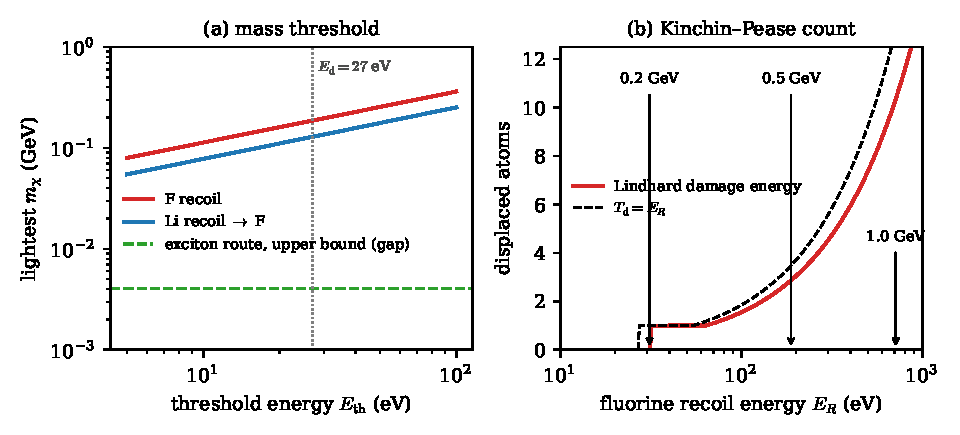
\includegraphics[width=\linewidth]{figures/ch16/fig16_6.pdf}
  \caption{F-center creation in LiF. (a) Lightest dark-matter mass that can create an F center, against the threshold energy of a step: a fluorine recoil above the threshold (red), a lithium recoil that passes the threshold energy to a fluorine neighbor in one head-on collision, transfer fraction 0.788 (blue), and the mass that deposits the band gap, \SI{14.2}{eV}, $\SI{4.0}{MeV}$, an upper bound on the threshold of the exciton route (green, dashed); \cref{eq:1.3-ERmax} with $v_{\mathrm{max}} = \num{2.650e-3}$. Dotted: $E_{\mathrm{d}} = \SI{27}{eV}$, the threshold used in binary-collision simulations of LiF. (b) Atoms displaced by a fluorine recoil in the Kinchin--Pease count with $E_{\mathrm{d}} = \SI{27}{eV}$, with the damage energy of the Lindhard partition for $Z = 9$, $A = 19$ (red; an extrapolation below about \SI{1}{keV}) and with no electronic loss (black, dashed). Arrows: the largest fluorine recoil energy for $\mchi = 0.2$, 0.5 and \SI{1.0}{GeV}, 31, 188 and \SI{711}{eV}.}
  \label{fig:16-lif}
\end{figure}

The number of vacancies a recoil makes follows from two classic estimates. The Lindhard partition splits a recoil of energy $E_R$ into an electronic share $y_LE_R$ and a damage energy $T_{\mathrm{d}} = (1 - y_L)E_R$, with $y_L$ of \cref{eq:16.6-lindhard} (\cref{sec:19.3}). The Kinchin--Pease count of \cref{sec:19.4-count}~\cite[Sect.~II]{cogswell2021passive} then gives no vacancy for $T_{\mathrm{d}} < E_{\mathrm{d}}$, one for $E_{\mathrm{d}} \le T_{\mathrm{d}} < 2E_{\mathrm{d}}$, and $T_{\mathrm{d}}/2E_{\mathrm{d}}$ above. The Lindhard partition and the Kinchin--Pease count are both rough at the energies of sub-GeV recoils. The Lindhard form already misses the measured ionization of silicon recoils of \SI{100}{eV} (\cref{app:E.23}), and its use for a fluorine recoil in a compound is a model choice. The Kinchin--Pease count ignores recombination and the direction dependence of $E_{\mathrm{d}}$. The two estimates set the scale of the yield, and \cref{we:16-fyield} uses them only to set that scale.

\begin{workedexample}{The yield of F centers per keV of fluorine recoil}\label{we:16-fyield}
Take a fluorine recoil of \SI{1}{keV} in LiF. With $Z = 9$ and $A = 19$, \cref{eq:16.6-lindhard} gives $k_L = 0.132$, $\epsilon_L = 0.0683$, $g_L = 2.21$ and $y_L = 0.226$: the recoil gives \SI{226}{eV} to the electrons and leaves a damage energy of \SI{774}{eV}. With $E_{\mathrm{d}} = \SI{27}{eV}$ the Kinchin--Pease count is $774/54 = 14.3$ displaced atoms, and 18.5 if no energy went to the electrons. The count does not say how the displacements divide between the two sublattices. If all displacements are on the anion sublattice, the count gives 14.3 fluorine vacancies per keV, an upper value; an equal share gives 7.2.

A fluorine vacancy becomes an F center only with an electron. The electronic share of \SI{226}{eV} makes at most $226/14.2 = 16$ electron--hole pairs, since each costs at least the gap, so at \SI{1}{keV} the electrons and the vacancies are comparable in number, before trapping and recombination take their share.

The balance between electrons and vacancies changes at the energies that sub-GeV dark matter reaches. A particle of \SI{0.5}{GeV} gives at most \SI{188}{eV}, a damage energy of \SI{155}{eV} and 2.9 displacements, but at most 2.3 pairs. At \SI{0.3}{GeV} the largest recoil is \SI{69}{eV}, about one displacement and at most 0.7 pairs; at \SI{0.2}{GeV}, \SI{31}{eV}, which reaches $T_{\mathrm{d}} = E_{\mathrm{d}}$ only without electronic loss. Near threshold a recoil therefore makes one vacancy and less than one free electron, and the charge factor $p_q$ in \cref{eq:16.6-yield} decides how many vacancies become F centers. The per-keV yield of the first paragraph, 7 to 14 fluorine vacancies, is an upper estimate that the four factors of \cref{eq:16.6-yield} reduce by amounts that no measurement fixes.
\end{workedexample}

\subsection{Bond breaking and cage escape}\label{sec:16.6-bond}

Take a diatomic molecule of atoms with masses $M_1$ and $M_2$ in a molecular solid, and let the dark matter strike atom 1. With the center of mass $\vect{R}_{\mathrm{CM}}$ and the bond vector $\vect{r} = \vect{R}_1 - \vect{R}_2$, the struck atom is at
\begin{equation*}
  \vect{R}_1 = \vect{R}_{\mathrm{CM}} + \frac{M_2}{M_{\mathrm{mol}}}\,\vect{r} = \vect{R}_{\mathrm{CM}} + \frac{\mu_{12}}{M_1}\,\vect{r} ,
\end{equation*}
with $M_{\mathrm{mol}} = M_1 + M_2$ and $\mu_{12} = M_1M_2/M_{\mathrm{mol}}$ the reduced mass of the bond. Assume that the forces of the neighbors act on the center of mass only, and depend neither on the length of the bond nor on its orientation. The Hamiltonian then splits into $H_{\mathrm{CM}} + H_{\mathrm{int}}$, the operators of the two parts commute, and so do their Heisenberg evolutions. The Fourier transform of the self correlation of the struck atom is its response (\cref{eq:D.32-I}). With $\vect{q}_{12} = (\mu_{12}/M_1)\vect{q}$ the kick on the bond vector, the self correlation factorizes,
\begin{equation*}
  \bigl\langle\ee^{-\ii\vect{q}\cdot\vect{R}_1(t)}\,\ee^{\ii\vect{q}\cdot\vect{R}_1}\bigr\rangle = \bigl\langle\ee^{-\ii\vect{q}\cdot\vect{R}_{\mathrm{CM}}(t)}\,\ee^{\ii\vect{q}\cdot\vect{R}_{\mathrm{CM}}}\bigr\rangle\,\bigl\langle\ee^{-\ii\vect{q}_{12}\cdot\vect{r}(t)}\,\ee^{\ii\vect{q}_{12}\cdot\vect{r}}\bigr\rangle ,
\end{equation*}
and a product in time is a convolution in frequency:
\begin{keyresult}[Response of an atom in a molecule]
\begin{equation}
  \begin{gathered}
  S_{11}(\vect{q},\omega) = \int\frac{\dd\omega'}{2\pi}\,S_{\mathrm{CM}}(\vect{q},\omega')\,S_{\mathrm{int}}(\vect{q}_{12},\omega - \omega') , \\
  S_{\mathrm{int}}(\vect{q}_{12},\omega) = 2\pi\sum_f\bigl|\langle f|\ee^{\ii\vect{q}_{12}\cdot\vect{r}}|0\rangle\bigr|^2\,\delta(\omega - E_f + E_0) .
  \end{gathered}
  \label{eq:16.6-conv}
\end{equation}
$S_{\mathrm{CM}}$ is the lattice response of a rigid molecule of mass $M_{\mathrm{mol}}$, and $S_{\mathrm{int}}$ the response of the bond to the kick $\vect{q}_{12}$ on its internal coordinate. The part of $S_{\mathrm{int}}$ with final states above the dissociation limit, $E_f - E_0 > E_{\mathrm{bond}}$, is the response for breaking the bond.
\end{keyresult}
\noindent The hypothesis holds best for molecules that rotate freely in the solid, with an internal motion that does not feel the cage. It fails for the fragments of a broken bond, which move through the cage and collide with its walls; the escape probability below accounts for that failure.

$S_{\mathrm{CM}}$ and $S_{\mathrm{int}}$ are both impulsive at the momenta that break bonds. A classical bond breaks when the kinetic energy $q_{12}^2/2\mu_{12}$ given to the internal motion exceeds $E_{\mathrm{bond}}$, which requires
\begin{equation}
  q \ge q_{\min} = \frac{M_1}{\mu_{12}}\,(2\mu_{12}E_{\mathrm{bond}})^{1/2} ,
  \label{eq:16.6-qmin}
\end{equation}
the threshold of Essig et al.~\cite[Eq.~(3.3)]{essig2017detection}. For H$_2$, with their $E_{\mathrm{bond}} = \SI{4.75}{eV}$, $q_{\min} = \SI{134}{keV}$, and a particle needs $\mchi \ge \SI{25.9}{MeV}$ to transfer it. The bond vibrates at $\omega_{\mathrm{vib}} = \SI{0.546}{eV}$~\cite{huber1979constants}, so the internal recoil parameter $E_{\mathrm{bond}}/\omega_{\mathrm{vib}}$ is 8.7, and the center-of-mass recoil, a few eV against intermolecular phonons of meV, is deep in the impulse regime of \cref{sec:11.4}. In the impulse approximation each factor of \cref{eq:16.6-conv} shifts the deposit by a Doppler term. The center of mass shifts it by $\vect{q}\cdot\vect{P}_{\mathrm{CM}}/M_{\mathrm{mol}}$, which changes the minimum velocity $\omega/q + q/2\mchi$ by $(\langle\omega\rangle_{\mathrm{CM}}/2M_{\mathrm{mol}})^{1/2}$ per standard deviation, $2\times10^{-6}$ for H$_2$ with an assumed $\langle\omega\rangle_{\mathrm{CM}} = \SI{10}{meV}$, against $v_{\mathrm{max}} = \num{2.650e-3}$. The center-of-mass shift does not decide whether the bond breaks and plays no further role. The internal factor shifts the energy given to the bond by $\vect{q}_{12}\cdot\vect{p}_{12}/\mu_{12}$, with $\vect{p}_{12}$ the relative momentum in the ground state, and that shift decides the outcome. In the impulse approximation the bond breaks when
\begin{equation}
  \frac{q_{12}^2}{2\mu_{12}} + \frac{\vect{q}_{12}\cdot\vect{p}_{12}}{\mu_{12}} > E_{\mathrm{bond}} .
  \label{eq:16.6-diss}
\end{equation}
Averaging over the ground state gives the dissociation probability of a kick $\vect{q}$. Essig et al.\ take the ground state of a free rotor, a Gaussian in the bond length $|\vect{r}|$ about its equilibrium value, isotropic in direction~\cite[Eq.~(3.12)]{essig2017detection}. With the harmonic width $(\mu_{12}\omega_{\mathrm{vib}})^{-1/2}$ the projection of $\vect{p}_{12}$ on $\hat{\vect{q}}$ has the root-mean-square value $(\mu_{12}\omega_{\mathrm{vib}}/6)^{1/2}$, \SI{6.53}{keV} or 1.75 times $\alpha m_e$ for H$_2$.

The published rates are limits of \cref{eq:16.6-conv,eq:16.6-diss}. With $S_{\mathrm{CM}}$ the free recoil of the molecule and $\vect{p}_{12} \to 0$, the deposit is $q^2/2M_{\mathrm{mol}} + \mu_{12}q^2/2M_1^2 = q^2/2M_1$, the minimum velocity is $q/2\mu_{\chi1}$, and the rate is the free recoil \cref{eq:11.4-LS} of atom 1 cut at $q_{\min}$, the classical rate of Essig et al.~\cite[Eq.~(4.3)]{essig2017detection}. Their quantum rate keeps the spread of the ground state, with plane-wave final states whose internal momentum is set by the energy above the dissociation limit, the improved Born approximation~\cite[Eqs.~(3.11), (3.17), (4.5)]{essig2017detection}. In that approximation the bond breaks when $|\vect{q}_{12} + \vect{p}_{12}|^2/2\mu_{12} > E_{\mathrm{bond}}$. The Born condition differs from \cref{eq:16.6-diss} by the initial kinetic energy of the bond, $\langle p_{12}^2\rangle/2\mu_{12} = \omega_{\mathrm{vib}}/4 = \SI{0.136}{eV}$ for H$_2$: the Born form counts the final kinetic energy of the fragments from zero, the impulse form counts the energy the kick adds.

\begin{limitbox}[Color-center creation and bond breaking][lim:16.6a]
The published color-center rate is the free nuclear recoil \cref{eq:11.4-LS} cut by a step at the displacement threshold, $\Theta(E_R - E_{\mathrm{d}})$~\cite[Eqs.~(1), (2), (5), (7)]{budnik2018direct}. The published classical bond-breaking rate is the free recoil of the struck atom cut at $q_{\min}$ of \cref{eq:16.6-qmin}~\cite[Eqs.~(3.3), (4.3)]{essig2017detection}.
\par\smallskip
{\centering
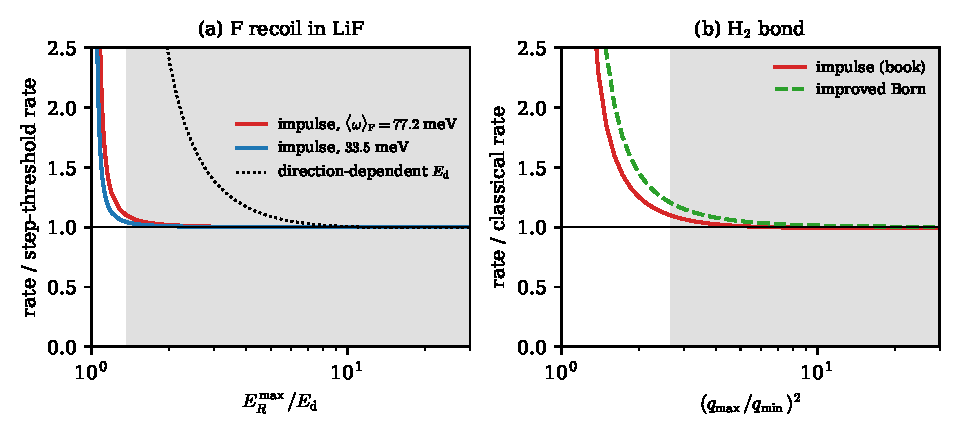
\includegraphics[width=\linewidth]{figures/ch16/limit16_6a.pdf}
\captionof{figure}{Rates from the impulse response of the bound target divided by the published forms, heavy mediator, standard halo, $T = 0$. (a) Fluorine recoils in LiF with $E_{\mathrm{d}} = \SI{27}{eV}$, against the ratio of the largest recoil energy to the threshold: \cref{eq:16.6-ccrate} with the yield a step at $\omega = E_{\mathrm{d}}$, for $\langle\omega\rangle_{\mathrm{F}} = \SI{77.2}{meV}$ (red, the top of the LiF optical band, an upper value) and \SI{33.5}{meV} (blue). Dotted: the direction-dependent threshold $E_{\mathrm{d}}(1 + a\sin4\theta\cos4\varphi)^2$ with $a = 0.4$, recoil directions isotropic in the crystal, divided by the step at $E_{\mathrm{d}}$. (b) H$_2$ as a free rotor: \cref{eq:16.6-conv} with \cref{eq:16.6-diss} over the Gaussian ground state (red) and with the improved Born condition (green, dashed), against $(q_{\max}/q_{\min})^2$, $q_{\max} = 2\mu_{\chi1}v_{\mathrm{max}}$. Gray: the red curve within \SI{10}{\percent} of one, $E_R^{\max} \ge 1.36\,E_{\mathrm{d}}$ ($\mchi \ge \SI{0.218}{GeV}$) in (a) and $(q_{\max}/q_{\min})^2 \ge 2.65$ ($\mchi \ge \SI{42.9}{MeV}$) in (b).}\label{fig:16-limit-cc}
\par}
\smallskip
Closer to threshold the color-center and bond-breaking rates both depend on the zero-point motion of the struck nucleus or bond and stay nonzero below the classical endpoint, and at every mass they still lack the yield factors of \cref{eq:16.6-yield} and the escape probability of the fragments of a bond, which multiply both curves.
\end{limitbox}

In \cref{lim:16.6a} the Doppler width changes the LiF rate by less than \SI{2}{\percent} once the largest recoil energy exceeds twice the threshold, and with the Doppler width the rate reaches the step-form rate for $E_R^{\max} = 1.1\,E_{\mathrm{d}}$ at a mass \SI{1.4}{\percent} lower. The directional structure of the threshold matters more: with the angular model of Budnik et al.\ the rate stays more than \SI{10}{\percent} away from the step value up to $E_R^{\max} = 4.8\,E_{\mathrm{d}}$, or $\mchi = \SI{0.41}{GeV}$, because the threshold surface reaches down to $0.36\,E_{\mathrm{d}}$. For H$_2$ the impulse rate equals the classical rate of $\mchi = \SI{27.2}{MeV}$ already at \SI{22.8}{MeV}, a shift of the mass scale by a factor 0.84; the improved Born rate does so at \SI{20.3}{MeV}, a factor 0.75.

A broken bond is not yet a signal. In a solid the two fragments start inside the cage of their neighbors, and they recombine unless they escape it; this recombination inside the cage is the cage effect of photochemistry. The rate of separated fragments is the rate of dissociating seeds times the escape probability $p_{\mathrm{esc}}(E_{\mathrm{int}},\hat{\vect{r}})$, which depends on the energy $E_{\mathrm{int}}$ the fragments share above the dissociation limit and on the direction of the bond relative to the cage. Electronic deposits break bonds as well: an excitation into a repulsive state, the antibonding $\sigma^*$ surface of the bond, dissociates the molecule without any nuclear kick, at the electronic thresholds of the molecular crystals of \cref{sec:16.4}. Neither $p_{\mathrm{esc}}$ nor the dissociation yields of these electronic states have been quantified at the momenta and temperatures of a dark-matter search.

\subsection{Measured yields and single-center readout}\label{sec:16.6-yields}

Of the inputs to \cref{eq:16.6-yield}, the displacement threshold is the one with measurements, and these fix only its lowest point. Electron irradiation of silicon sees damage set in at $12.9 \pm \SI{0.6}{eV}$, where density-functional molecular dynamics puts the minimum of $E_{\mathrm{d}}(\hat{\vect{r}})$ (\cref{sec:7.4}). The shape of $p_{\mathrm{FP}}$ above the minimum is a computed quantity: the defect probability becomes nonzero below the average threshold and approaches one only at two to three times the average threshold~\cite[Sect.~II]{cogswell2021passive}. In materials where an interstitial recombines with its own vacancy a direction-resolved threshold is not even well defined (\cref{app:E.11}). For ionic crystals the measured responses are those of dense tracks at room temperature: fast neutrons, $\gamma$ rays of $^{60}$Co, and the $\alpha$ and triton tracks of neutron capture on $^6$Li~\cite{araujo2026nuclear}. The aggregates that LiF forms along these dense tracks are stable for months in vacuum at room temperature and anneal away at \SI{350}{\celsius}~\cite[Sect.~III]{araujo2026nuclear}. None of these measurements isolates a single recoil of tens to hundreds of eV, and none is made at millikelvin temperatures.

A single-center readout at millikelvin temperatures must work without aggregation. A sub-GeV recoil makes one to three vacancies (\cref{we:16-fyield}), and at \SI{10}{mK} they do not move, so the emitting aggregates read in LiF tracks do not form and the readout must find a single F center. In LiF that center has no observed luminescence~\cite{guerreroperez2025first}, so it must be found through its absorption near \SI{5.1}{eV}, in the ultraviolet, or converted into a state that emits. For an emitting center in a light-guiding rod, Budnik et al.\ estimate $5\times10^5$ detected photons in \SI{e3}{s} and a detection limit of about one new center among $10^5$ existing ones~\cite[footnote~1]{budnik2018direct}. The existing centers set the background. Commercial crystals are not certified below a defect concentration of $10^{-9}$, and annealing at up to \SI{1000}{\celsius} removes many of the existing centers~\cite{budnik2018direct}; fluorescence measurements of LiF put an upper limit of $10^{-12}$ to $10^{-10}$ on the centers present before irradiation~\cite{cogswell2021passive}. At millikelvin temperatures the readout light must also deposit less heat than the detector tolerates; none of these estimates addresses this heat load.

Four yields remain open at millikelvin temperatures: the conversion $p_{\mathrm{FH}}$ of a self-trapped exciton into a Frenkel pair, the survival $p_{\mathrm{surv}}$ of a close pair with the charge factor $p_q$ at recoil energies of tens to hundreds of eV, the efficiency $f_{\mathrm{opt}}$ of reading a single center, and the escape $p_{\mathrm{esc}}$ of the fragments of a bond with the yields of repulsive electronic states. Each can be measured directly. Neutrons scattered at a tagged angle in LiF at \SI{10}{mK} give recoils of known energy, and counting single F centers per tagged recoil measures the product $p_{\mathrm{FP}}p_{\mathrm{surv}}p_qf_{\mathrm{opt}}$ as a function of $E_R$. X-rays of \SI{5.9}{keV} absorbed at millikelvin temperatures give $p_{\mathrm{FH}}$ from the F-center yield per absorbed energy together with the quenching of the exciton luminescence. The photodissociation quantum yield of a molecular crystal at millikelvin temperatures, with the fragments detected by infrared absorption, gives $p_{\mathrm{esc}}$.

\section{Glasses, random media and two-level systems}\label{sec:16.7}

A superconducting resonator made on a film of thermally grown SiO$_2$ loses a fraction $3\times10^{-4}$ of its stored energy per radian at \SI{6}{GHz} and below \SI{100}{mK}, when it holds only a few photons~\cite[Table~I]{oconnell2008microwave}. At higher power or temperature the loss falls. The absorbers are groups of atoms in the glass that can sit in either of two configurations and tunnel between them, typically $10^{20}$ per eV and cm$^3$, with splittings that reach down to micro-electronvolts. At these energies a crystal has only its long acoustic phonons. The same systems absorb a dark photon of mass \SI{25}{\micro eV} as readily as a microwave photon of that energy, and a dark-matter particle that scatters in the glass can flip one of them. A glass is also the plainest example of a random medium. Its disorder raises two further questions: how its vibrations absorb a dark photon once momentum conservation no longer selects one optical phonon, and when a light particle that scatters coherently off a whole body can be treated in the Born approximation. The same tunneling systems release heat at millikelvin temperatures, and their kinetics are the subject of \cref{sec:16.8}.

\subsection{The standard tunneling model}\label{sec:16.7-stm}

Let $|\mathrm{L}\rangle$ and $|\mathrm{R}\rangle$ be the ground states of a group of atoms localized in the two wells of a double-well potential. In their span the Hamiltonian is \cref{eq:C.20-H} without the bath,
\begin{equation}
  H_{\mathrm{TLS}} = \tfrac12\Delta_{\mathrm{as}}\,\sigma_z - \tfrac12\Delta_0\,\sigma_x ,
  \qquad \Delta_{\mathrm{tl}} = \bigl(\Delta_{\mathrm{as}}^2 + \Delta_0^2\bigr)^{1/2} ,
  \label{eq:16.7-H}
\end{equation}
with the Pauli matrices of \cref{app:C.20} in the localized basis, the asymmetry $\Delta_{\mathrm{as}}$ between the two wells, the tunneling amplitude $\Delta_0$ and the splitting $\Delta_{\mathrm{tl}}$ of the eigenstates, the two-level splitting of \cref{sec:2.5}. The tunneling amplitude is exponentially small in the barrier, $\Delta_0 = \omega_{\mathrm{w}}\ee^{-\lambda_{\mathrm{tun}}}$, with $\omega_{\mathrm{w}} \sim$ the vibration energy in one well. For a particle of mass $M_{\mathrm{tun}}$ crossing a barrier of height $V_{\mathrm{b}}$ between wells a distance $d_{\mathrm{tun}}$ apart, the tunneling exponent is $\lambda_{\mathrm{tun}} = (d_{\mathrm{tun}}/2)(2M_{\mathrm{tun}}V_{\mathrm{b}})^{1/2}$~\cite[Sect.~II]{meissner2021acoustic}. In the eigenbasis the matrix $\sigma_z$, which measures in which well the atoms sit, becomes
\begin{equation}
  \sigma_z = \frac{\Delta_{\mathrm{as}}}{\Delta_{\mathrm{tl}}}\,\tau_z + \frac{\Delta_0}{\Delta_{\mathrm{tl}}}\,\tau_x ,
  \label{eq:16.7-rot}
\end{equation}
with $\tau_z$ and $\tau_x$ the Pauli matrices of the eigenstates and the sign of $\tau_x$ fixed by the phases of the eigenvectors. A perturbation that couples to the position of the atoms therefore drives transitions with the amplitude $\Delta_0/\Delta_{\mathrm{tl}}$: a system with $\Delta_0 \ll \Delta_{\mathrm{as}}$ has its eigenstates localized in the two wells, and the perturbation cannot move it from one to the other.

In a glass every system has its own $\Delta_{\mathrm{as}}$ and $\lambda_{\mathrm{tun}}$. The standard tunneling model of Phillips and of Anderson, Halperin and Varma takes both to be independent and uniformly distributed, with density $\bar P$ per unit asymmetry, unit exponent and unit volume~\cite[Eq.~(8)]{muller2019towards}. A system and its mirror image are the same system, so we count $\Delta_{\mathrm{as}} \ge 0$ only; this convention defines $\bar P$, and with both signs counted every rate below would carry a factor 2. Changing variables from $(\Delta_{\mathrm{as}}, \lambda_{\mathrm{tun}})$ to $(\Delta_{\mathrm{tl}}, \Delta_0)$, with $\dd\lambda_{\mathrm{tun}} = -\dd\Delta_0/\Delta_0$ and $\partial\Delta_{\mathrm{as}}/\partial\Delta_{\mathrm{tl}} = \Delta_{\mathrm{tl}}/\Delta_{\mathrm{as}}$ at fixed $\Delta_0$, gives
\begin{equation}
  P(\Delta_{\mathrm{tl}},\Delta_0) = \frac{\bar P\,\Delta_{\mathrm{tl}}}{\Delta_0\,(\Delta_{\mathrm{tl}}^2 - \Delta_0^2)^{1/2}} ,
  \qquad 0 < \Delta_0 \le \Delta_{\mathrm{tl}} ,
  \label{eq:16.7-P}
\end{equation}
the distribution of Ref.~\cite[Eq.~(12)]{meissner2021acoustic}. Its integral over $\Delta_0$ diverges logarithmically at small $\Delta_0$, and the number of systems per unit splitting depends on a lower cutoff of the tunneling amplitude that no experiment fixes. A transition probability, however, carries the weight $(\Delta_0/\Delta_{\mathrm{tl}})^2$ of \cref{eq:16.7-rot}, and
\begin{equation}
  \int_0^{\Delta_{\mathrm{tl}}}\dd\Delta_0\,P(\Delta_{\mathrm{tl}},\Delta_0)\,\frac{\Delta_0^2}{\Delta_{\mathrm{tl}}^2} = \bar P\int_0^1\frac{u\,\dd u}{(1 - u^2)^{1/2}} = \bar P ,
  \label{eq:16.7-norm}
\end{equation}
with $u = \Delta_0/\Delta_{\mathrm{tl}}$. The systems that dominate the count do not couple, and those that couple are counted by $\bar P$ alone, at every splitting. \Cref{fig:16-tls}(a) shows the two densities.

\begin{figure}[tbp]
  \centering
  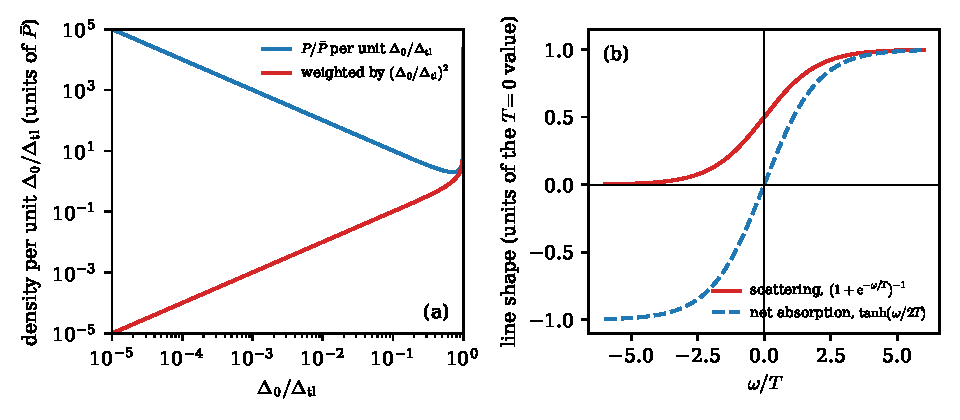
\includegraphics[width=\linewidth]{figures/ch16/fig16_7.pdf}
  \caption{The standard tunneling model. (a) Density of two-level systems per unit $u = \Delta_0/\Delta_{\mathrm{tl}}$ at fixed splitting, in units of $\bar P$: $1/[u(1 - u^2)^{1/2}]$ (blue), whose integral grows as $\ln(2/u_{\min})$ with the lower cutoff $u_{\min}$. Weighted by the squared transition amplitude $u^2$ (red), it integrates to one, \cref{eq:16.7-norm}; \SI{87}{\percent} of that comes from $u > 0.5$. (b) Line shapes of the ensemble at temperature $T$, in units of their $T = 0$ values. Red: the scattering structure factor $(1 + \ee^{-\omega/T})^{-1}$ of \cref{eq:16.7-S}, nonzero for $\omega < 0$ through the thermal population of the upper level; blue, dashed: the net absorption of a classical field, $\tanh(\omega/2T)$, \cref{eq:16.7-chires}.}
  \label{fig:16-tls}
\end{figure}

A strain field and an electric field both shift the energies of the two wells. The atoms move between configurations with different elastic and electric dipoles. To first order the asymmetry becomes $\Delta_{\mathrm{as}} + 2\gamma_{\mathrm{TLS}}u_{\mathrm{d}} + 2\vect{p}_{\mathrm{TLS}}\cdot\vect{E}$, with $u_{\mathrm{d}}$ the component of the strain tensor $u_{\alpha\beta}$ along the deformation of the defect, $\gamma_{\mathrm{TLS}}$ its deformation potential and $\vect{p}_{\mathrm{TLS}}$ half the difference of the electric dipoles of the two configurations~\cite[Eq.~(16)]{muller2019towards}. The perturbation is
\begin{equation}
  H_1 = \bigl(\gamma_{\mathrm{TLS}}u_{\mathrm{d}} + \vect{p}_{\mathrm{TLS}}\cdot\vect{E}\bigr)\,\sigma_z \equiv bF\,\sigma_z ,
  \label{eq:16.7-H1}
\end{equation}
where $F$ stands for the applied field ($u_{\mathrm{d}}$ or one component of $\vect{E}$) and $b$ for the coupling to it. By \cref{eq:16.7-rot} it has a transverse part, which drives transitions at $\omega = \Delta_{\mathrm{tl}}$, and a longitudinal part, which modulates the splitting.

The transverse part gives the resonant response. The power a field $F\cos\omega t$ deposits per unit volume is $\tfrac12\omega\chi''(\omega)F^2$, with $\chi''$ the absorptive part of the susceptibility of the coupled quantity $b\sigma_z$. For one system the golden rule of \cref{sec:2.1} gives an absorption rate from the lower level and an equal rate of stimulated emission from the upper one, and the populations of \cref{sec:2.5} differ by $p_0 - p_1 = \tanh(\Delta_{\mathrm{tl}}/2T)$. Hence $\chi''(\omega) = \pi b^2(\Delta_0/\Delta_{\mathrm{tl}})^2\tanh(\Delta_{\mathrm{tl}}/2T)\,\delta(\omega - \Delta_{\mathrm{tl}})$ for $\omega > 0$, where the delta function stands for the Lorentzian of \cref{eq:2.4-lorentz} with the width of the system, small against $\omega$ and $T$ in an insulating glass at millikelvin temperatures. Summing over the ensemble with \cref{eq:16.7-P,eq:16.7-norm},
\begin{equation}
  \chi''_{\mathrm{res}}(\omega) = \pi\bar P\,\langle b^2\rangle\,\tanh\frac{\omega}{2T} ,
  \label{eq:16.7-chires}
\end{equation}
independent of $\omega$, with $\langle b^2\rangle$ averaged over the orientations of the systems. Its two physical cases are the dielectric loss and the acoustic loss. For the electric field the orientation average is $\langle(\vect{p}_{\mathrm{TLS}}\cdot\hat{\vect{E}})^2\rangle = p_{\mathrm{TLS}}^2/3$, and in Heaviside--Lorentz units the polarization is $\chi\vect{E}$, so the imaginary part of the permittivity is $\chi''$ itself. Against the real part $\varepsilon_r$ of the glass, the loss tangent is
\begin{equation}
  \tan\delta(\omega,T) = \frac{\varepsilon_2}{\varepsilon_r} = \tan\delta_0\,\tanh\frac{\omega}{2T} , \qquad
  \tan\delta_0 = \frac{\pi\bar P\,p_{\mathrm{TLS}}^2}{3\varepsilon_r} ,
  \label{eq:16.7-tand}
\end{equation}
the low-power loss tangent $\tan\delta_0$ at $T \to 0$. For a sound wave of polarization $j$, longitudinal or transverse, the coupling is the deformation potential $\gamma_j$ and the elastic modulus $\rho_Tc_j^2$ takes the place of $\varepsilon_r$, so the internal friction is $Q^{-1} = \pi C_j\tanh(\omega/2T)$, with the tunneling strength $C_j = \bar P\gamma_j^2/\rho_Tc_j^2$~\cite[Eqs.~(5), (6)]{buchenau2020sound}. Both are the response of the standard tunneling model to a classical field~\cite[Eqs.~(4), (12), (13), (15)]{meissner2021acoustic}. In vitreous silica $C = 2.6\times10^{-4}$ on average over the two polarizations~\cite[Table~I]{buchenau2020sound}, and Golding, Graebner and Schutz find $C_{\mathrm{l}} = 1.9\times10^{-4}$ and $C_{\mathrm{t}} = 2.0\times10^{-4}$ at \SI{500}{MHz}, as quoted by Buchenau et al.~\cite[Sect.~III]{buchenau2020sound}.

The longitudinal part of \cref{eq:16.7-H1}, $bF(\Delta_{\mathrm{as}}/\Delta_{\mathrm{tl}})\tau_z$, shifts the splitting by $2bF\Delta_{\mathrm{as}}/\Delta_{\mathrm{tl}}$. In equilibrium the population difference would follow the shifted splitting at once; in fact it relaxes toward it at the rate $\varGamma_1 = 1/\tau_1$ of the system. The static susceptibility of the coupled quantity is $2b^2(\Delta_{\mathrm{as}}/\Delta_{\mathrm{tl}})^2\,\partial_{\Delta_{\mathrm{tl}}}\tanh(\Delta_{\mathrm{tl}}/2T)$, and a population that relaxes with one time constant turns it into the Debye form $\chi_{\mathrm{rel}}(\omega) = \chi_{\mathrm{rel}}(0)/(1 - \ii\omega\tau_1)$, whose absorptive part is $\chi_{\mathrm{rel}}(0)\,\omega\tau_1/(1 + \omega^2\tau_1^2)$~\cite[Eq.~(6)]{meissner2021acoustic}. In an insulating glass $\varGamma_1$ is set by the emission and absorption of one thermal phonon,
\begin{equation}
  \varGamma_1 = K_{\mathrm{ph}}\,\Delta_{\mathrm{tl}}^3\Bigl(\frac{\Delta_0}{\Delta_{\mathrm{tl}}}\Bigr)^2\coth\frac{\Delta_{\mathrm{tl}}}{2T} , \qquad
  K_{\mathrm{ph}} = \frac{1}{2\pi\rho_T}\Bigl(\frac{\gamma_{\mathrm{l}}^2}{c_{\mathrm{LA}}^5} + \frac{2\gamma_{\mathrm{t}}^2}{c_{\mathrm{TA}}^5}\Bigr) ,
  \label{eq:16.7-tau1}
\end{equation}
which \cref{sec:16.8} derives~\cite[Eq.~(7)]{meissner2021acoustic}. Summed over the ensemble and divided by the resonant value at $T = 0$, the full loss is
\begin{equation}
  \frac{\tan\delta}{\tan\delta_0} = \tanh\frac{\omega}{2T} + \frac{2}{\pi}\int_0^\infty\frac{\dd\Delta_{\mathrm{tl}}}{2T}\,\mathrm{sech}^2\frac{\Delta_{\mathrm{tl}}}{2T}\int_0^1\dd u\,\frac{(1 - u^2)^{1/2}}{u}\,\frac{\omega\tau_1}{1 + \omega^2\tau_1^2} ,
  \label{eq:16.7-relax}
\end{equation}
with $u = \Delta_0/\Delta_{\mathrm{tl}}$ and $\tau_1 = 1/\varGamma_1$ from \cref{eq:16.7-tau1}; the same ratio holds for $Q^{-1}/\pi C_j$. The relaxation part has two limits. Since $\tau_1^{-1} \propto u^2$, the fastest systems are those with $u = 1$. When they relax fast, $\omega\tau_1(u = 1) \ll 1$, the $u$ integral is dominated by the slower systems with $u^2 \sim \omega\tau_1(u = 1)$, where $\omega\tau_1 \sim 1$; it equals $\pi/4$, and the relaxation part saturates at $\tfrac12$, the tunneling plateau $Q^{-1} = \pi C/2$~\cite[Eq.~(10)]{buchenau2020sound}. When even the fastest systems relax slowly, $\omega\tau_1(u = 1) \gg 1$, the integrand is $1/\omega\tau_1$, the $u$ integral gives $\tfrac13$, and the energy integral gives $\int_0^\infty y^3\,\dd y/\sinh y = \pi^4/8$, so the relaxation part is $(\pi^3/12)K_{\mathrm{ph}}T^3/\omega$. Compared to the resonant part, $\omega/2T$ at $T \gg \omega$, it grows as $T^4/\omega^2$.

\begin{limitbox}[Two-level response to a classical strain or field][lim:16.7a]
The resonant loss of the standard tunneling model, $\tan\delta = \tan\delta_0\tanh(\omega/2T)$ with $\tan\delta_0 = \pi\bar Pp_{\mathrm{TLS}}^2/3\varepsilon_r$, and $Q^{-1} = \pi C_j\tanh(\omega/2T)$ for sound~\cite[Eqs.~(4), (12), (13), (15)]{meissner2021acoustic}.
\par\smallskip
{\centering
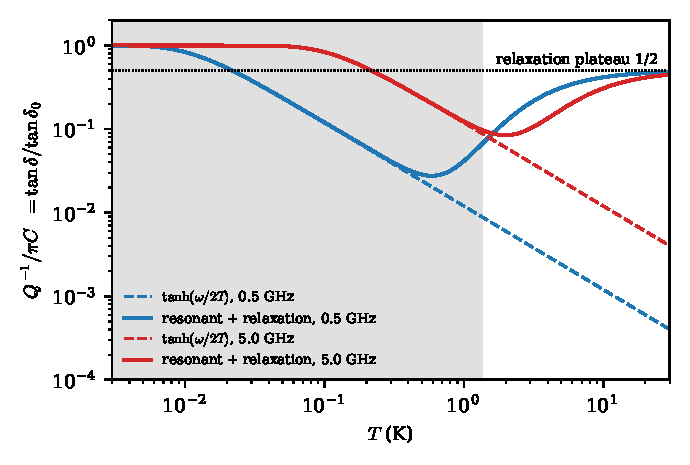
\includegraphics[width=0.82\linewidth]{figures/ch16/limit16_7a.pdf}
\captionof{figure}{Loss of the ensemble in vitreous silica, divided by its value at $T = 0$, against temperature, at \SI{0.5}{GHz} (blue) and \SI{5}{GHz} (red). Dashed: $\tanh(\omega/2T)$. Solid: resonant plus relaxation part, \cref{eq:16.7-relax}, with the one-phonon rate \cref{eq:16.7-tau1} for $\rho_T = \SI{2.2}{g.cm^{-3}}$, $c_{\mathrm{LA}} = 5.8$ and $c_{\mathrm{TA}} = \SI{3.8}{km.s^{-1}}$~\cite[Table~I]{buchenau2020sound}, an assumed $\gamma_{\mathrm{l}} = \SI{1}{eV}$ and $\gamma_{\mathrm{l}}/\gamma_{\mathrm{t}} = 1.6$~\cite{zhou2015generic}, so that $K_{\mathrm{ph}} = \SI{4.63e4}{eV^{-2}}$. Dotted: the relaxation plateau. Gray: the full loss within \SI{10}{\percent} of the tanh law at \SI{5}{GHz}, $T < \SI{1.36}{K}$ (\SI{0.43}{K} at \SI{0.5}{GHz}).}\label{fig:16-limit-tls}
\par}
\smallskip
Above these temperatures the population of slowly relaxing systems lags the field, and the loss rises toward the plateau $\tan\delta_0/2$ instead of falling as $\omega/2T$.
\end{limitbox}

\Cref{lim:16.7a} puts the relaxation correction where the low-temperature estimate puts it: \SI{10}{\percent} of the resonant loss at $T = [0.6\,\omega^2/(\pi^3K_{\mathrm{ph}})]^{1/4}$, which is \SI{1.34}{K} at \SI{5}{GHz} against \SI{1.36}{K} from the full integral. At \SI{10}{mK} the relaxation part at \SI{5}{GHz} is $4\times10^{-9}$ of the resonant one. The value of $\gamma_{\mathrm{l}}$ enters only through $K_{\mathrm{ph}}$, and since the crossover temperature scales as $K_{\mathrm{ph}}^{-1/4}$, a deformation potential twice as large moves it down by a factor $2^{1/2}$. The tunneling model has its own limits at these temperatures: above about \SI{2}{K}, relaxation by several phonons adds to \cref{eq:16.7-tau1}~\cite[Sect.~II]{meissner2021acoustic}. The second correction is saturation. A field strong enough to drive transitions faster than the systems relax equalizes the two populations and removes the resonant loss; for sound the resonant term falls as $[1 + I/I_{\mathrm{c}}]^{-1/2}$ with the intensity $I$, and the critical intensity is $\sim10^{-7}\,\si{W.cm^{-2}}$~\cite[Eq.~(8)]{buchenau2020sound}. This is why the resonator loss falls at high power and why $\tan\delta_0$ is the low-power value. In practice the tunneling parameters, the distributions of $\Delta_{\mathrm{as}}$ and $\lambda_{\mathrm{tun}}$, the deformation potentials and the dipole moments, are computed from ensembles of model glasses, found by searching their energy landscapes for pairs of nearby minima (\cref{app:E.22}). The computed $\bar Pp_{\mathrm{TLS}}^2$ is then checked against the measured $\tan\delta_0$ of the same preparation.

\subsection{Dark-photon absorption on two-level systems}\label{sec:16.7-dp}

A dark photon of mass $m_\phi$ is absorbed at the rate per unit target mass $\mathcal{R} = (\rho_\chi/\rho_T)\zeta^2L(m_\phi)$, with $L = \Imag(-1/\varepsilon)$ the loss function at $\vect{p}_\phi \to 0$ (\cref{eq:10.7-dp}). The momentum $\vect{p}_\phi \approx m_\phi v$ of a dark photon of \SI{25}{\micro eV} is $3\times10^{-8}\,\si{eV}$ for $v = \SI{354}{km.s^{-1}}$, a wavelength of about \SI{40}{m}, so the local dielectric function of the glass is all we need. For a glass with $\varepsilon = \varepsilon_r(1 + \ii\tan\delta)$ the loss function is $\tan\delta/[\varepsilon_r(1 + \tan^2\delta)]$, and with \cref{eq:16.7-tand},
\begin{keyresult}[Dark-photon absorption on two-level systems]
\begin{equation}
  \mathcal{R} = \frac{\rho_\chi}{\rho_T}\,\zeta^2\,\frac{\tan\delta_0}{\varepsilon_r}\,\tanh\frac{m_\phi}{2T}\,\bigl[1 + \mathcal{O}(\tan^2\delta_0)\bigr] .
  \label{eq:16.7-dp}
\end{equation}
The rate per unit mass is independent of $m_\phi$ wherever $m_\phi \gg 2T$, and it is fixed by two measured numbers, the low-power loss tangent and the permittivity.
\end{keyresult}
\noindent The factor $\tanh(m_\phi/2T)$ appears once. It is the population difference of the absorbing systems, and the net rate already subtracts the stimulated emission that the dark-matter field drives from the upper level, just as the dielectric loss does; a second thermal factor from the field would count that subtraction twice. The in-medium suppression $1/\varepsilon_r$ is the factor $1/|\varepsilon|^2$ of \cref{eq:10.7-dp} times the $\varepsilon_r$ in $\varepsilon_2 = \varepsilon_r\tan\delta$: the field inside the glass is screened, and the absorbers respond to the screened field. And the dark-matter field drives each system far below saturation. At the coupling that \cref{we:16-tls-dp} finds for three events per kg-year, the field $\zeta(2\rho_\chi)^{1/2}$ of \cref{sec:11.8} gives a Rabi frequency below $6\times10^{-7}\,\si{s^{-1}}$ for a dipole of \SI{1.1}{D}, against a relaxation rate of $10^6\,\si{s^{-1}}$ for a system with $\Delta_{\mathrm{tl}} = m_\phi$ at \SI{6}{GHz}.

What the two-level systems add is a loss that is flat in frequency, from the lowest masses at which $m_\phi$ exceeds $2T$ up to the energies at which the flat distribution \cref{eq:16.7-P} ceases to hold. The loss tangents that fix the rate are measured near \SI{6}{GHz} (\SI{25}{\micro eV}) and below \SI{100}{mK}, and they depend on how the oxide was made. Thermal SiO$_2$ has $\tan\delta_0 = 3.0$ to $3.3\times10^{-4}$, and oxide deposited from a plasma $2.7$ to $2.9\times10^{-3}$ in lumped-element resonators~\cite[Table~I]{oconnell2008microwave}. A second deposited oxide reached $5\times10^{-3}$~\cite{martinis2005decoherence}. Such films are a few hundred nanometers thick, and no millikelvin value has been measured for bulk fused silica.

\begin{workedexample}{The dark-photon rate on thermal SiO$_2$}\label{we:16-tls-dp}
Take thermal SiO$_2$ with $\tan\delta_0 = 3\times10^{-4}$, an assumed static permittivity $\varepsilon_r = 3.9$, and $\rho_T = \SI{2.2}{g.cm^{-3}}$, at $T = \SI{10}{mK}$ ($T = \SI{0.862}{\micro eV}$). A dark photon of \SI{6}{GHz}, $m_\phi = \SI{24.81}{\micro eV}$, has $m_\phi/2T = 14.4$, so $\tanh(m_\phi/2T) = 1$ to eight digits, and the loss function is $L = 3\times10^{-4}/3.9 = \num{7.69e-5}$. The prefactor is $\rho_\chi/\rho_T = (\SI{0.3}{GeV.cm^{-3}})/(\SI{2.2}{g.cm^{-3}}) = \SI{0.136}{GeV/g}$, which divided by $\hbar$ is $2.07\times10^{23}$ per gram per second. Then
\begin{equation*}
  \mathcal{R} = \num{5.03e29}\,\zeta^2\ \text{per kg-year} ,
\end{equation*}
and three events in one kg-year need $\zeta = \num{2.44e-15}$. The upper end of the measured range, $3.3\times10^{-4}$, raises the rate by 1.10, and the deposited oxide with $5\times10^{-3}$ by 16.7, which lowers $\zeta$ by a factor 0.24. At \SI{100}{mK} the thermal factor drops to 0.894, which is why a loss tangent quoted at that temperature must be divided by 0.894 to give $\tan\delta_0$.

The target mass is the problem. A film of \SI{1}{\micro m} on \SI{100}{cm^2} weighs \SI{22}{mg}, and three events in a year then need $\zeta = \num{5.2e-13}$. Each absorption leaves \SI{24.8}{\micro eV} in one two-level system, which decays by emitting a phonon of that energy. The loss tangent also fixes $\bar Pp_{\mathrm{TLS}}^2 = 3\varepsilon_r\tan\delta_0/\pi$ and nothing else: with $\bar P = \SI{1.2e20}{eV^{-1}.cm^{-3}}$, the value that the polarization-averaged $C = 2.6\times10^{-4}$ implies for $\gamma_{\mathrm{l}} = \SI{1}{eV}$, \cref{eq:16.7-tand} requires $p_{\mathrm{TLS}} = 0.23\,e\,\text{\AA} = \SI{1.1}{D}$.
\end{workedexample}

\begin{limitbox}[Dark-photon absorption on two-level systems][lim:16.7b]
$\mathcal{R} = (\rho_\chi/\rho_T)\zeta^2\tan\delta_0\tanh(m_\phi/2T)/\varepsilon_r$, the loss function $\Imag(-1/\varepsilon) = \varepsilon_2/|\varepsilon|^2$ of \cref{eq:10.7-dp} with the electric loss of the tunneling model~\cite[Eq.~(20)]{muller2019towards}.
\par\smallskip
{\centering
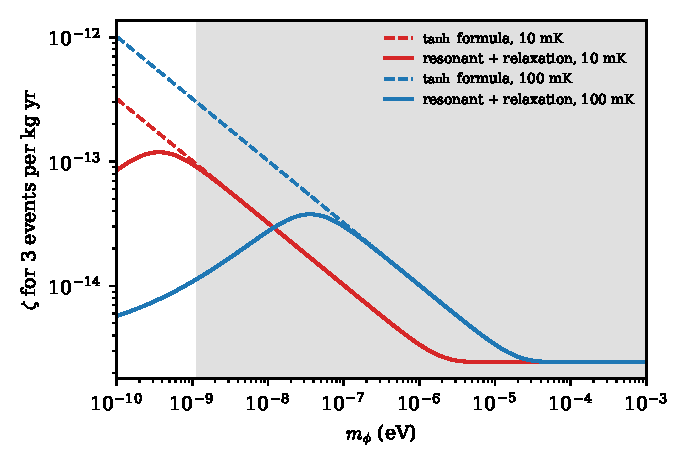
\includegraphics[width=0.82\linewidth]{figures/ch16/limit16_7b.pdf}
\captionof{figure}{Kinetic mixing for three absorptions per kg-year on thermal SiO$_2$ ($\tan\delta_0 = 3\times10^{-4}$, $\varepsilon_r = 3.9$, $\rho_T = \SI{2.2}{g.cm^{-3}}$), against the dark-photon mass, at \SI{10}{mK} (red) and \SI{100}{mK} (blue). Dashed: \cref{eq:16.7-dp}. Solid: $\varepsilon_2/|\varepsilon|^2$ with $\varepsilon_2$ from the resonant plus relaxation loss \cref{eq:16.7-relax}, $K_{\mathrm{ph}}$ as in \cref{fig:16-limit-tls}. Gray: within \SI{10}{\percent} at \SI{10}{mK}, $m_\phi > \SI{1.15}{neV}$ (\SI{0.28}{MHz}); at \SI{100}{mK} the bound moves to \SI{115}{neV}.}\label{fig:16-limit-dp}
\par}
\smallskip
Below these masses the relaxation of systems with splittings near $T$ absorbs more than the resonant systems at $\Delta_{\mathrm{tl}} = m_\phi$, whose population difference vanishes as $m_\phi/2T$.
\end{limitbox}

\noindent The mass of \cref{lim:16.7b} scales as $T^2$: with $\tanh(m_\phi/2T) \approx m_\phi/2T$ and the low-temperature relaxation part $(\pi^3/12)K_{\mathrm{ph}}T^3/m_\phi$, the two are in the ratio $(\pi^3/6)K_{\mathrm{ph}}T^4/m_\phi^2$, which reaches 0.1 at $m_\phi \propto T^2$. Above a millielectronvolt the vibrations of the glass absorb more than its two-level systems (\cref{sec:16.7-ir}).

\subsection{Dark-matter scattering on two-level systems}\label{sec:16.7-scat}

A dark-matter particle that couples to the electron density sees a two-level system through the change of that density between the two configurations. Projected on $|\mathrm{L}\rangle$ and $|\mathrm{R}\rangle$, the density operator at momentum $\vect{q}$ is $\tfrac12(n_{\mathrm{LL}} + n_{\mathrm{RR}}) - \tfrac12f_{\mathrm{TLS}}(\vect{q})\,\sigma_z$, up to terms of relative order $\ee^{-\lambda_{\mathrm{tun}}}$, with the vertex
\begin{equation}
  f_{\mathrm{TLS}}(\vect{q}) = \langle\mathrm{R}|n_e(\vect{q})|\mathrm{R}\rangle - \langle\mathrm{L}|n_e(\vect{q})|\mathrm{L}\rangle .
  \label{eq:16.7-f}
\end{equation}
The first term is the static density and scatters elastically; the second flips the system with the amplitude of \cref{eq:16.7-rot}, $|\langle e|n_e(\vect{q})|g\rangle|^2 = \tfrac14|f_{\mathrm{TLS}}|^2(\Delta_0/\Delta_{\mathrm{tl}})^2$. The structure factor of \cref{eq:2.5-golden} sums this over systems, with the weights $p_0$ and $p_1$ of \cref{sec:2.5} for absorption at $\omega = \Delta_{\mathrm{tl}}$ and emission at $\omega = -\Delta_{\mathrm{tl}}$, and with \cref{eq:16.7-P,eq:16.7-norm} the ensemble gives
\begin{equation}
  S(\vect{q},\omega) = \frac{\pi}{2}\,\bar P\,\bigl\langle|f_{\mathrm{TLS}}(\vect{q})|^2\bigr\rangle\,\frac{1}{1 + \ee^{-\omega/T}} ,
  \label{eq:16.7-S}
\end{equation}
flat in $\omega$ inside the band of the two-level systems and obeying detailed balance, \cref{eq:2.5-db}, as \cref{fig:16-tls}(b) shows. The average runs over the systems and their orientations.

The vertex has two parts. The atoms that tunnel carry their electrons from one well to the other, the core term. And the surrounding glass relaxes elastically around each configuration, which moves all its electrons, the host term. For the host term take the defect as an elastic dipole. In configuration R it exerts on the glass a force dipole that differs from that of L by $-2\gamma_{\mathrm{TLS}}$ along its deformation, since the energy of a force dipole $\mathsf{D}$ in a strain is $-\sum_{\alpha\beta}\mathsf{D}_{\alpha\beta}u_{\alpha\beta}$ and the asymmetry shifts by $2\gamma_{\mathrm{TLS}}u_{\mathrm{d}}$. In an isotropic continuum the static displacement field of a force dipole has longitudinal Fourier component $\vect{q}\cdot\tilde{\vect{u}}(\vect{q}) = -\ii\,\hat{\vect{q}}\cdot\mathsf{D}\cdot\hat{\vect{q}}/\rho_Tc_{\mathrm{LA}}^2$, and since the adiabatic electrons follow the atoms, the electron density changes by $\delta n_e(\vect{q}) = \ii\nd_e\,\vect{q}\cdot\tilde{\vect{u}}$ with $\nd_e$ the density of all electrons. Hence
\begin{equation}
  f_{\mathrm{host}} = \frac{2\nd_e\,\hat{\vect{q}}\cdot\gamma_{\mathrm{TLS}}\cdot\hat{\vect{q}}}{\rho_Tc_{\mathrm{LA}}^2} ,
  \qquad
  \bar P\,\bigl\langle|f_{\mathrm{host}}|^2\bigr\rangle = \frac{4\nd_e^2\,C_{\mathrm{l}}}{\rho_Tc_{\mathrm{LA}}^2} ,
  \label{eq:16.7-host}
\end{equation}
where the orientation average of $(\hat{\vect{q}}\cdot\gamma_{\mathrm{TLS}}\cdot\hat{\vect{q}})^2$ is $\gamma_{\mathrm{l}}^2$, the coupling to longitudinal strain. The deformation potential drops out of the product: the host term of the scattering rate is fixed by the measured tunneling strength $C_{\mathrm{l}}$, not by the loss tangent. The form holds in a window of momentum transfers. The momentum transfer must be static, $q \gg \omega/c_{\mathrm{LA}}$; for $\omega$ near $c_{\mathrm{LA}}q$ the elastic response has a pole, and the process becomes the emission of a real phonon that the two-level system absorbs later, which belongs to the phonon channel of \cref{sec:11.1}. The wavelength must also be long against the defect and the atomic spacing, where continuum elasticity holds. No dielectric factor is added: the adiabatic density already contains the screening of the electrons.

For the core term the simplest model moves one oxygen ion, with its eight electrons, rigidly by $\vect{d}$. With the origin at the midpoint, $f_{\mathrm{core}} = 8(\ee^{\ii\vect{q}\cdot\vect{d}/2} - \ee^{-\ii\vect{q}\cdot\vect{d}/2}) = 16\ii\sin(\vect{q}\cdot\vect{d}/2)$, and its orientation average is $\langle|f_{\mathrm{core}}|^2\rangle = 128[1 - \sin(qd)/qd]$. The core amplitude is imaginary and the static host amplitude is real, so the two add without interference, for every orientation and not only on average; an off-center core would restore a cross term. For a displacement along $\hat{\vect{q}}$ the two are equal near $q_\times = |f_{\mathrm{host}}|/(8d)$, where the host term stops dominating; with the orientation-averaged core, $\langle|f_{\mathrm{core}}|^2\rangle^{1/2} \simeq 4.62\,qd$, the crossing moves up by $\sqrt3$.

With a heavy mediator, $\mathfrak{D}_{ee} = \pi\sigmae/\mu_{\chi e}^2$ and the structure factor \cref{eq:16.7-S} in the isotropic rate \cref{eq:10.1-rateiso}, the minimum velocity is $q/2\mchi$ up to $\omega/q$, negligible for $\omega \lesssim \SI{0.1}{meV}$, and a $q$-independent vertex leaves $\int q\,\dd q\,\eta(q/2\mchi) = 2\mchi^2\langle v\rangle$. The rate is
\begin{equation}
  \frac{\dd\mathcal{R}}{\dd\omega} = \frac{\rho_\chi}{\mchi\rho_T}\,\langle v\rangle\,\sigmae\Bigl(1 + \frac{\mchi}{m_e}\Bigr)^2\,\frac{\bar P\langle|f_{\mathrm{TLS}}|^2\rangle}{4\,(1 + \ee^{-\omega/T})} ,
  \label{eq:16.7-rate}
\end{equation}
per unit energy and target mass, a cross-section $\sigmae(1 + \mchi/m_e)^2|f_{\mathrm{TLS}}|^2(\Delta_0/\Delta_{\mathrm{tl}})^2/4$ per system. The factor $(1 + \mchi/m_e)^2 = \mchi^2/\mu_{\chi e}^2$ converts the reference cross-section on a free electron into the cross-section on a heavy target. For a $q$-dependent core vertex the $q$ integral is done with $\eta$.

Consider amorphous SiO$_2$ at $\mchi = \SI{1}{MeV}$ and $\sigmae = \SI{e-38}{cm^2}$. Thirty electrons per formula unit at \SI{2.2}{g.cm^{-3}} give $\nd_e = \SI{6.62e23}{cm^{-3}}$, and $\rho_Tc_{\mathrm{LA}}^2 = \SI{7.40e10}{Pa} = \SI{4.62e23}{eV.cm^{-3}}$. With the measured longitudinal $C_{\mathrm{l}} = 1.9\times10^{-4}$, \cref{eq:16.7-host} gives $\bar P\langle|f_{\mathrm{host}}|^2\rangle = \SI{7.20e20}{eV^{-1}.cm^{-3}}$, and with the halo of \cref{tab:1-shm}, $\langle v\rangle = \SI{354.1}{km.s^{-1}}$, and $(1 + \mchi/m_e)^2 = 8.74$, the host term is $6.6\times10^{-3}$ per kg, day and meV. The core term needs $\bar P$ itself. For an assumed $\gamma_{\mathrm{l}} = \SI{1}{eV}$, $\bar P = C_{\mathrm{l}}\rho_Tc_{\mathrm{LA}}^2/\gamma_{\mathrm{l}}^2 = \SI{8.8e19}{eV^{-1}.cm^{-3}}$, $|f_{\mathrm{host}}| = 2.86$, and one oxygen moving by \SI{1}{\angstrom} adds $1.6\times10^{-2}$, 2.5 times the host term. The total,
\begin{equation*}
  \frac{\dd\mathcal{R}}{\dd\omega} \approx 2.3\times10^{-2}\ \text{per kg, day and meV} \qquad (\mchi = \SI{1}{MeV},\ \sigmae = \SI{e-38}{cm^2}),
\end{equation*}
is flat over the band of the two-level systems, and over $0 < \omega < \SI{0.1}{meV}$ it amounts to $2.3\times10^{-3}$ events per kg-day. The polarization-averaged $C = 2.6\times10^{-4}$ would raise both terms by 1.37, to $3.1\times10^{-2}$ per kg, day and meV.

This number is an estimate, uncertain by about a factor 3. The heavy-mediator weight $q\,\eta(q/2\mchi)$ has its median at $q = \SI{1.73}{keV}$, where $qd = 0.88$ for $d = \SI{1}{\angstrom}$. The host and core terms cross lower, at $q_\times = \SI{0.71}{keV}$ for a displacement along $\hat{\vect{q}}$ and \SI{1.2}{keV} on orientation average. Most of the rate therefore comes from momentum transfers outside the window of \cref{eq:16.7-host}, near the scale at which the glass stops being a continuum. The core term is a rigid ion, which misses the redistribution of the valence electrons of the moving oxygen, and one geometry stands for many. Both are replaced by the density difference \cref{eq:16.7-f} from two self-consistent calculations of the same glass cell, averaged over an ensemble of systems. Whatever its value, the rate is small because $\bar P$ times the band of energies, about $10^{16}$ systems per cm$^3$, is a small number of targets, and each takes at most \SI{0.1}{meV}. Thin films under a sensor hold far less mass still and matter as absorbers of phonons and as sources of delayed heat (\cref{sec:16.8}), not as targets.

\subsection{Vibrational absorption of glasses}\label{sec:16.7-ir}

In a crystal a dark photon is absorbed on phonons only at the zone-center optical frequencies, where its tiny momentum matches a mode (\cref{sec:11.8}). A glass has no zone center. Every vibrational mode can carry a dipole, and the absorption is spread over the whole vibrational spectrum~\cite{bloch2026dark}. The rate is still $\mathcal{R} = (\rho_\chi/\rho_T)\zeta^2L(m_\phi)$, now with the dielectric function of the vibrations of the glass~\cite[Eq.~(2)]{bloch2026dark}, and the question is what fixes $L$ at the lowest masses.

Take one configuration of the glass in the harmonic approximation, with modes $\nu$ of frequency $\omega_\nu$, eigenvectors $\vect{e}_{I\nu}$ normalized over all $N$ atoms, masses $M_I$ and Born charges $Z^*_I$. Its dielectric function has the rank-one form of \cref{sec:11.8}, with the Hessian of the glass in place of the dynamical matrix,
\begin{equation}
  \varepsilon(\omega) = \varepsilon_\infty + \frac{e^2}{\Vol}\sum_\nu\frac{|p_\nu|^2}{\omega_\nu^2 - \omega^2 - \ii\omega\varGamma_\nu} ,
  \qquad p_\nu = \sum_I\frac{\hat{\boldsymbol{\epsilon}}\cdot Z^*_I\cdot\vect{e}_{I\nu}}{M_I^{1/2}} ,
  \label{eq:16.7-epsglass}
\end{equation}
for a field along $\hat{\boldsymbol{\epsilon}}$ and mode widths $\varGamma_\nu$. For narrow modes the imaginary part is $\varepsilon_2(\omega) = (\pi e^2/2\omega\Vol)\sum_\nu|p_\nu|^2\delta(\omega - \omega_\nu)$. With the vibrational density of states $g(\omega)$ normalized to one, $\sum_\nu\delta(\omega - \omega_\nu) = 3Ng(\omega)$, and with the infrared coupling $C^{\mathrm{IR}}(\omega)$, the mean of $|p_\nu|^2$ over the modes at frequency $\omega$,
\begin{equation}
  \varepsilon_2(\omega) = \frac{3\pi e^2\nd_{\mathrm{at}}}{2\omega}\,g(\omega)\,C^{\mathrm{IR}}(\omega) .
  \label{eq:16.7-eps2}
\end{equation}
The absorption coefficient $\alpha_{\mathrm{abs}} = \omega\varepsilon_2/n_r$, with $n_r = \varepsilon_r^{1/2}$ the refractive index, is then a product of the density of states and a coupling, the form in which infrared spectroscopy of glasses is analyzed~\cite[Eq.~(2) and text before Eq.~(1)]{taraskin2006universal}.

Below the Ioffe--Regel frequency $\omega_{\mathrm{IoR}}$, the frequency at which the mean free path of a vibration falls to one wavelength, the modes are still sound waves, scattered weakly by the disorder. For a plane wave of branch $\nu$ with sound speed $c_\nu$, wavevector $\vect{k}$ and polarization $\hat{\vect{e}}_\nu$, every atom moves with the same velocity, $\vect{e}_{I\nu} = \hat{\vect{e}}_\nu\ee^{\ii\vect{k}\cdot\vect{x}_I}(M_I/N\bar M)^{1/2}$ with $\bar M$ the mean atomic mass. The masses cancel in $p_\nu$, which becomes a Fourier component of the field of Born charges, and averaged over the modes at fixed $\omega = c_\nu k$,
\begin{equation}
  C^{\mathrm{IR}}(\omega) = \frac{1}{\bar M}\sum_\nu\hat w_\nu\,S^Z_\nu(\omega/c_\nu) ,
  \qquad S^Z_\nu(k) = \frac1N\Bigl\langle\Bigl|\sum_I\hat{\boldsymbol{\epsilon}}\cdot Z^*_I\cdot\hat{\vect{e}}_\nu\,\ee^{\ii\vect{k}\cdot\vect{x}_I}\Bigr|^2\Bigr\rangle ,
  \label{eq:16.7-CIR}
\end{equation}
with $\hat w_\nu = c_\nu^{-3}/\sum_{\nu'}c_{\nu'}^{-3}$ the fraction of modes at fixed $\omega$ in branch $\nu$, as in \cref{eq:E.19-CIR}. The behavior of $S^Z_\nu$ at small $k$ decides the low-frequency absorption. A crystal has $S^Z_\nu(k) = 0$ for acoustic modes as $k \to 0$, since the Born charges of a cell add to zero. In a glass the charges fluctuate from site to site. If they obey only global neutrality, uncorrelated fluctuations leave $S^Z_\nu(0^+)$ equal to the mean square fluctuation of the projected charge, a constant. If instead they are neutral within every local unit, as within the SiO$_4$ tetrahedra of silica, the sum is that of dipoles and $S^Z_\nu \propto k^2$. Expanding to second order,
\begin{equation}
  C^{\mathrm{IR}}(\omega) = A^{\mathrm{IR}} + B^{\mathrm{IR}}\omega^2 , \qquad
  A^{\mathrm{IR}} = \frac{1}{\bar M}\sum_\nu\hat w_\nu S^Z_\nu(0^+) , \quad
  B^{\mathrm{IR}} = \frac{1}{\bar M}\sum_\nu\frac{\hat w_\nu S^{Z\prime\prime}_\nu(0)}{2c_\nu^2} ,
  \label{eq:16.7-AB}
\end{equation}
the law Taraskin, Simdyankin, Elliott, Neilson and Lo found in terahertz spectra of glasses~\cite[Eq.~(1)]{taraskin2006universal}. Their fit to vitreous silica at room temperature writes $\alpha_{\mathrm{abs}} = (A^{\mathrm{IR}} + B^{\mathrm{IR}}\tilde\omega^2)g(\tilde\omega)$ in spectroscopic units, with $\alpha_{\mathrm{abs}}$ and the wavenumber $\tilde\omega = \omega/2\pi c$ in cm$^{-1}$ and $g$ normalized per cm$^{-1}$. It gives $A^{\mathrm{IR}} = \SI{4000}{cm^{-2}}$ and $B^{\mathrm{IR}} = 0.3$, dimensionless, with the Debye density of states of a \SI{330}{K} Debye temperature~\cite[Fig.~1]{taraskin2006universal}. Harmonic absorption is net absorption and does not depend on temperature, but a room-temperature spectrum also contains anharmonic and relaxational absorption whose size at millikelvin temperatures has not been separated; there the fit is a model value.

\begin{limitbox}[Glass absorption below the Ioffe--Regel frequency][lim:16.7d]
$\alpha_{\mathrm{abs}}(\omega) = (A^{\mathrm{IR}} + B^{\mathrm{IR}}\tilde\omega^2)\,g(\tilde\omega)$ for $\omega < \omega_{\mathrm{IoR}}$~\cite[Eq.~(1)]{taraskin2006universal}, inserted in the rate $(\rho_\chi/\rho_T)\zeta^2\Imag(-1/\varepsilon)$~\cite[Eq.~(2)]{bloch2026dark}.
\par\smallskip
{\centering
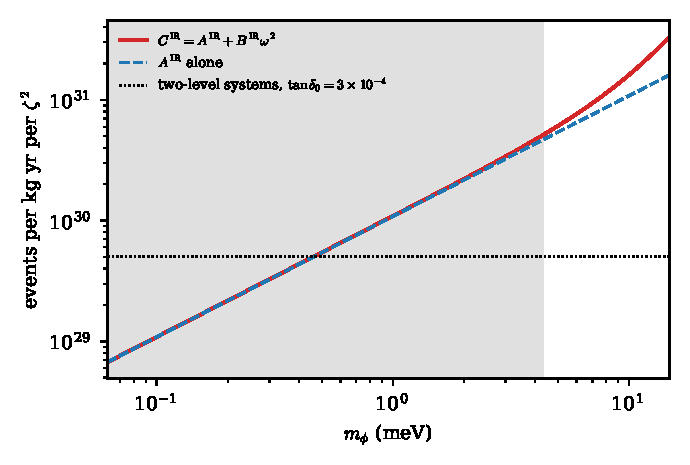
\includegraphics[width=0.82\linewidth]{figures/ch16/limit16_7d.pdf}
\captionof{figure}{Dark-photon absorptions per kg-year per $\zeta^2$ in vitreous silica against the mass, from \cref{eq:16.7-eps2} with $C^{\mathrm{IR}} = A^{\mathrm{IR}} + B^{\mathrm{IR}}\omega^2$ (red) and with the constant term alone (blue, dashed). Inputs: the terahertz fit $A^{\mathrm{IR}} = \SI{4000}{cm^{-2}}$, $B^{\mathrm{IR}} = 0.3$ of Taraskin et al., a Debye density of states with $\Theta_{\mathrm{D}} = \SI{330}{K}$, $\varepsilon_r = 3.9$ and $\rho_T = \SI{2.2}{g.cm^{-3}}$. Dotted: two-level absorption, \cref{eq:16.7-dp}, for thermal SiO$_2$ at saturation. Gray: below the Ioffe--Regel frequency of silica, $\omega/2\pi c \approx \SI{35}{cm^{-1}}$ (\SI{4.3}{meV}), where the $B$ term is at most \SI{9}{\percent} of the $A$ term.}\label{fig:16-limit-ir}
\par}
\smallskip
Above $\omega_{\mathrm{IoR}}$ the modes are no longer plane waves, $S^Z_\nu$ at one wavevector no longer describes them, and the coupling departs from $A^{\mathrm{IR}} + B^{\mathrm{IR}}\omega^2$ in a way that depends on the glass.
\end{limitbox}

\Cref{lim:16.7d} shows how the two channels of a glass divide the masses. With $\varepsilon_2 = n_r\alpha_{\mathrm{abs}}/(2\pi\tilde\omega)$, the vibrational absorption grows as $\omega$ times $C^{\mathrm{IR}}$. At \SI{1.24}{meV} ($\tilde\omega = \SI{10}{cm^{-1}}$) it gives $\alpha_{\mathrm{abs}} = \SI{0.10}{cm^{-1}}$, $\varepsilon_2 = \num{3.1e-3}$ and $1.4\times10^{30}\zeta^2$ absorptions per kg-year. It equals the two-level absorption of thermal SiO$_2$ at \SI{0.46}{meV}, and that of the deposited oxide with $\tan\delta_0 = 5\times10^{-3}$ at \SI{6.4}{meV}, an extrapolation above $\omega_{\mathrm{IoR}}$. The constant term carries the low-frequency absorption of silica entirely: the curvature term reaches the constant only at $\tilde\omega = (A^{\mathrm{IR}}/B^{\mathrm{IR}})^{1/2} = \SI{115}{cm^{-1}}$, three times above $\omega_{\mathrm{IoR}}$. That constant is the incoherent sum of random charges, and a model of the glass that makes every tetrahedron neutral by construction misses it (\cref{app:E.19}). Bloch, Knapen, Li, Madden and Marocco propose amorphous membranes for masses of 50 to \SI{200}{meV}, above $\omega_{\mathrm{IoR}}$, where the mean free path of a mode is shorter than its wavelength and the absorption follows from the measured or computed $\varepsilon(\omega)$ of \cref{eq:16.7-epsglass}~\cite{bloch2026dark}. The same random couplings give a broadband absorption in a crystal with isotope disorder, which \cref{sec:11.6} treats.

\subsection{Random media and the Born limit}\label{sec:16.7-random}

A dark-matter particle of \SI{20}{eV} moving at $v = 10^{-3}$ has a de Broglie wavelength $2\pi/\mchi v$ of about \SI{60}{\micro m}. A momentum transfer $\sim\mchi v$ cannot resolve atoms, and the particle scatters off the smoothed density $\nd(\vect{r})$ of nucleons of a whole body. Liu, Matsumoto, Sheng and Xing pointed out that a random two-phase material scatters such particles far more strongly than a homogeneous one~\cite{liu2025coherence}. In the first Born approximation for the body, the amplitudes of all nucleons add with their phases, and for a spin-independent interaction
\begin{equation}
  \frac{\dd\sigma_{\mathrm{tot}}}{\dd\Omega_q} = \frac{\dd\sigma_{\chi N}}{\dd\Omega_q}\,\Bigl|\int\dd^3r\,\ee^{\ii\vect{q}\cdot\vect{r}}\,\nd(\vect{r})\Bigr|^2 ,
  \label{eq:16.7-born}
\end{equation}
the coherent sum of \cref{sec:2.2} with the nucleus replaced by the body~\cite[Eq.~(2)]{liu2025coherence}. Write $\nd = \nd_0 + \delta\nd$ with $\nd_0$ the mean nucleon density, and average over the random structure. The cross term vanishes, and the two remaining terms are the homogeneous body, $\nd_0^2|\int_{\Vol}\dd^3r\,\ee^{\ii\vect{q}\cdot\vect{r}}|^2$, which falls as $(qR)^{-4}$ for a sphere of radius $R$ once $qR \gg 1$, and the fluctuations, $\int\dd^3r_1\dd^3r_2\,\ee^{\ii\vect{q}\cdot(\vect{r}_2 - \vect{r}_1)}\langle\delta\nd(\vect{r}_1)\delta\nd(\vect{r}_2)\rangle$. For a correlation that decays as $\langle\delta\nd(\vect{r}_1)\delta\nd(\vect{r}_2)\rangle = \delta\nd^2\ee^{-|\vect{r}_2 - \vect{r}_1|/\xi_{\mathrm{c}}}$ over a correlation length $\xi_{\mathrm{c}}$, the transform $\int\dd^3r\,\ee^{\ii\vect{q}\cdot\vect{r}}\ee^{-r/\xi_{\mathrm{c}}} = 8\pi\xi_{\mathrm{c}}^3/(1 + q^2\xi_{\mathrm{c}}^2)^2$ times the volume $\Vol = 4\pi R^3/3$ gives, per squared number of nucleons $\nd_0^2\Vol^2$,
\begin{equation}
  |F_{\mathrm{fluc}}(q)|^2 = \frac{\delta\nd^2}{\nd_0^2}\,\frac{6\,\xi_{\mathrm{c}}^3}{R^3(1 + q^2\xi_{\mathrm{c}}^2)^2} ,
  \label{eq:16.7-Ffluc}
\end{equation}
for $R \gg \xi_{\mathrm{c}}$, the result of Ref.~\cite[Eqs.~(9)--(12)]{liu2025coherence}. The body acts as a collection of incoherent clusters of size $\xi_{\mathrm{c}}$, each scattering coherently. At $qR \gg 1$ and $q\xi_{\mathrm{c}} \gg 1$ the sphere-averaged homogeneous term is $9/[2(qR)^4]$, and the ratio of the two is $(4/3)(R/\xi_{\mathrm{c}})(\delta\nd/\nd_0)^2$. For the Ti--6Al--4V alloy of the test masses of the MICROSCOPE satellite test of the equivalence principle, the authors infer $\nd_0 = \SI{2.69e24}{cm^{-3}}$ and $\delta\nd = \SI{7.29e22}{cm^{-3}}$ from the phase fractions of its microstructure~\cite[Eq.~(14)]{liu2025coherence}. Then $(\delta\nd/\nd_0)^2 = 7\times10^{-4}$, and for that value the homogeneous term the authors drop is the larger one below a few hundred eV on an equal-mass sphere.

A large coherent cross-section, however, means a strong interaction with the medium, and the Born approximation for a whole body is not the Born approximation for one nucleus. At wavelengths long against the spacing of nuclei, the medium acts on the particle as an optical potential. It is the sum of the pseudopotentials $2\pi b_{\chi N}/\mu_{\chi N}$ of the nucleons, with $b_{\chi N}$ the scattering length, $\sigma_{\chi N} = 4\pi b_{\chi N}^2$, and $\mu_{\chi N} \approx \mchi$ for a light particle:
\begin{equation}
  V_{\mathrm{opt}} = \frac{2\pi b_{\chi N}\nd_0}{\mu_{\chi N}} .
  \label{eq:16.7-Vopt}
\end{equation}
The plane wave inside the body is undistorted only if this potential is small against the kinetic energy, $|V_{\mathrm{opt}}| \ll E_{\mathrm{kin}} = \mchi v^2/2$. Squaring $|b_{\chi N}| \ll \mchi^2v^2/4\pi\nd_0$ gives the condition on the cross-section,
\begin{equation}
  \sigma_{\chi N} \ll \sigma_{\mathrm{crit}} = \frac{\mchi^4v^4}{4\pi\nd_0^2} ,
  \qquad \frac{|V_{\mathrm{opt}}|}{E_{\mathrm{kin}}} = \Bigl(\frac{\sigma_{\chi N}}{\sigma_{\mathrm{crit}}}\Bigr)^{1/2} .
  \label{eq:16.7-scrit}
\end{equation}
Since $\sigma_{\mathrm{crit}} \propto v^4$, the condition must hold over the velocities that dominate the observable, not at one speed. The homogeneous term of \cref{eq:16.7-born} contains the scattering of the wave by the surface of the body. For a planar face its first-order form can be compared with the exact reflection off a potential step, which shows where the first-order treatment of the medium breaks down. For a wave whose kinetic energy of motion normal to the face is $E_n$, the wavenumber inside is $k' = k(1 - V_{\mathrm{opt}}/E_n)^{1/2}$ and the reflectance is $R_{\mathrm{refl}} = |(k - k')/(k + k')|^2$, total for $V_{\mathrm{opt}} > E_n$. Expanding $k'$ to first order in $V_{\mathrm{opt}}$ gives the Born value $(V_{\mathrm{opt}}/4E_n)^2$, the square of the first-order amplitude of the step.

\begin{limitbox}[Random media and the Born limit][lim:16.7c]
First Born approximation for a whole body, $\dd\sigma_{\mathrm{tot}}/\dd\Omega_q = (\dd\sigma_{\chi N}/\dd\Omega_q)|\int\dd^3r\,\ee^{\ii\vect{q}\cdot\vect{r}}\nd(\vect{r})|^2$, with the fluctuation form factor \cref{eq:16.7-Ffluc}~\cite[Eqs.~(2), (9)--(12), (14)]{liu2025coherence}.
\par\smallskip
{\centering
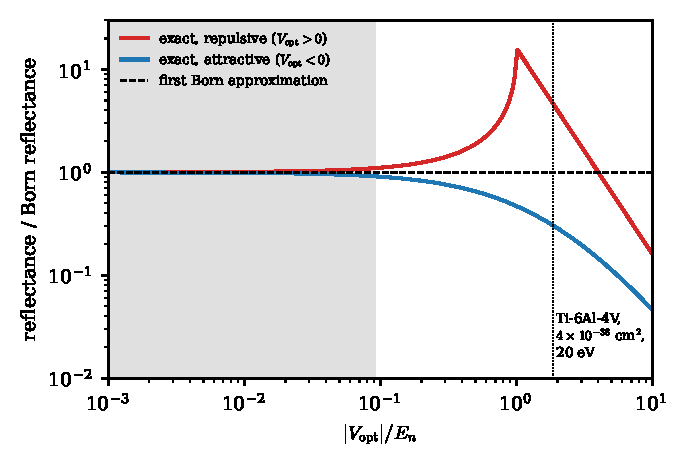
\includegraphics[width=0.82\linewidth]{figures/ch16/limit16_7c.pdf}
\captionof{figure}{Exact reflectance of a planar face of a homogeneous medium with optical potential \cref{eq:16.7-Vopt}, divided by its first Born approximation $(V_{\mathrm{opt}}/4E_n)^2$, against $|V_{\mathrm{opt}}|/E_n$, for a repulsive (red) and an attractive (blue) medium. $E_n$ is the kinetic energy of the motion normal to the face. Gray: the ratio within \SI{10}{\percent} of one, $|V_{\mathrm{opt}}|/E_n < 0.092$. Dotted: $V_{\mathrm{opt}}/E_{\mathrm{kin}} = 1.86$, the value at $\sigma_{\chi N} = \SI{4e-38}{cm^2}$, $\mchi = \SI{20}{eV}$, $v = 10^{-3}$ in Ti--6Al--4V ($\nd_0 = \SI{2.69e24}{cm^{-3}}$).}\label{fig:16-limit-born}
\par}
\smallskip
Beyond $|V_{\mathrm{opt}}| \approx E_n$ a repulsive body reflects every particle that reaches it, and the force on it scales with the optical potential of each material, not with the square of its density fluctuations.
\end{limitbox}

\noindent The leading correction is linear: the ratio of \cref{lim:16.7c} is $1 + V_{\mathrm{opt}}/E_n$ for small $V_{\mathrm{opt}}/E_n$, \SI{1}{\percent} at $V_{\mathrm{opt}}/E_n = 0.01$, of opposite sign for the two signs of the potential. Below $\sigma_{\mathrm{crit}}$ the uniform part of the medium only shifts the wavenumber inside, $k \to k'$, a phase that drops out of the fluctuation term once the wave is distorted by it, and the fluctuation cross-section keeps corrections of relative order $V_{\mathrm{opt}}/E_{\mathrm{kin}}$. In Ti--6Al--4V at $\mchi = \SI{20}{eV}$, \cref{eq:16.7-scrit} gives $\sigma_{\mathrm{crit}} = \SI{1.16e-38}{cm^2}$ at $v = 10^{-3}$, \SI{2.41e-38}{cm^2} at $v = \num{1.2e-3}$ and \SI{5.7e-37}{cm^2} at the largest laboratory speed $v_{\mathrm{max}} = \num{2.650e-3}$. Liu et al.\ quote a reach of $\sigma_{\chi N} \approx \SI{4e-38}{cm^2}$ near \SI{20}{eV} from the MICROSCOPE bound on differential acceleration~\cite[Sect.~IV]{liu2025coherence}, where $|V_{\mathrm{opt}}|/E_{\mathrm{kin}} = 1.86$ at $v = 10^{-3}$ and 1.29 at $v = \num{1.2e-3}$, before the projection on the normal of a face lowers $E_n$ further. At that cross-section the first-order treatment of the medium does not apply to the speeds near the peak of the distribution. Whether the true force on the test masses is larger or smaller than the Born estimate depends on the sign of $b_{\chi N}$, on reflection at the faces and on the composition difference of the two masses. Until the force is computed by transfer matrices over the faces and the velocity distribution, a bound from this channel is a conjecture.

\subsection{Open problems for glass targets}\label{sec:16.7-open}

For a given film the parameters of the standard tunneling model are known only in combination: the loss tangent fixes $\bar Pp_{\mathrm{TLS}}^2$, the acoustic loss $\bar P\gamma_{\mathrm{l}}^2$ and $\bar P\gamma_{\mathrm{t}}^2$, and neither fixes $\bar P$; the core term, the relaxation corrections and the kinetics of \cref{sec:16.8} need all three. For the films of real detectors (amorphous Al$_2$O$_3$ in junctions, SiO$_2$ and SiN$_x$ under sensors, amorphous WSi) these have not been measured on the same sample. Beyond the values, the model itself is an assumption: that $\Delta_{\mathrm{as}}$ and $\lambda_{\mathrm{tun}}$ are independent and flat, at every energy from the lowest masses to the top of the band, and that the systems do not interact. Its successes, the linear specific heat and the logarithmic shift of the sound velocity, test averages, not the distributions, and the ratio $\gamma_{\mathrm{l}}/\gamma_{\mathrm{t}}$, between 1.44 and 1.84 in 18 glasses, is nearly universal without the model giving a reason~\cite{zhou2015generic}. One film measured three ways would settle the first question: the dielectric loss, the acoustic loss, and the strain and field dependence of single systems resolved in a resonator, which give $\gamma_{\mathrm{TLS}}$ and $p_{\mathrm{TLS}}$ directly~\cite{muller2019towards}. The second needs the distributions computed for a model glass of stated preparation.

\section{Two-level systems at millikelvin}\label{sec:16.8}

One gram of fused silica cooled to \SI{10}{mK} is still giving off \SI{46}{pW} an hour later, and the power falls only as $1/t$ (\cref{we:16-heat}). For a detector held at \SI{10}{mK} this is a heat load that lasts for weeks. The heat comes from the tunneling two-level systems of \cref{sec:16.7}. Each was in equilibrium at a few kelvin, and each gives up its excess energy when it next relaxes, which for a defect behind a thick barrier takes hours or years. The same relaxation rates decide how fast a two-level system in a sensor film absorbs the energy of a phonon and returns it, and they are the kinetics behind the delayed signals of \cref{sec:19.6}. The defect is the two-configuration system of \cref{eq:C.20-H}, treated in the spin--boson language of \cref{app:C.20}.

\subsection{Relaxation by one phonon}\label{sec:16.8-phonon}

A two-level system relaxes when it passes from the upper to the lower of its two eigenstates and gives the splitting to its surroundings. The environment couples to the configuration through $\tfrac12\sigma_z X$, with $X = \sum_k\lambda_k(d_k + d_k^\dagger)$ the bath coordinate of \cref{eq:C.20-H}. By \cref{eq:16.7-rot} only the off-diagonal element $\Delta_0/\Delta_{\mathrm{tl}}$ of $\sigma_z$ in the eigenbasis changes the state; the diagonal part shifts the splitting by the fluctuating bath and contributes only to the dephasing. By the golden rule of \cref{sec:2.1} the emission of a bath quantum of energy $\Delta_{\mathrm{tl}}$ has the rate $2\pi\sum_k(\Delta_0\lambda_k/2\Delta_{\mathrm{tl}})^2(n_{\mathrm{B}} + 1)\,\delta(\Delta_{\mathrm{tl}} - \omega_k)$, and absorption has the same rate with $n_{\mathrm{B}}$ in place of $n_{\mathrm{B}} + 1$. A population difference relaxes at the sum of the two, which carries $2n_{\mathrm{B}} + 1 = \coth(\Delta_{\mathrm{tl}}/2T)$:
\begin{equation}
  \varGamma_1 = \frac12\Bigl(\frac{\Delta_0}{\Delta_{\mathrm{tl}}}\Bigr)^2 J_{\mathrm{s}}(\Delta_{\mathrm{tl}})\,\coth\frac{\Delta_{\mathrm{tl}}}{2T} .
  \label{eq:16.8-golden}
\end{equation}
The bath enters only through its spectral density $J_{\mathrm{s}}(\omega) = \pi\sum_k\lambda_k^2\delta(\omega - \omega_k)$ of \cref{eq:C.20-J} at the splitting. The rate is first order in $J_{\mathrm{s}}$, and it holds as long as $\varGamma_1 \ll \Delta_{\mathrm{tl}}$, so that the eigenstates are defined; its upward and downward parts obey detailed balance (\cref{sec:2.5}).

A long acoustic wave couples through the strain term of \cref{eq:16.7-H1}, and the deformation potential depends on the orientation of the defect relative to the wave. As in \cref{sec:16.7}, $\gamma_{\mathrm{l}}^2$ and $\gamma_{\mathrm{t}}^2$ are its mean squares over orientations for a longitudinal wave and for each transverse wave; acoustic experiments on glasses give about \SI{1}{eV}~\cite[Sect.~IV\,A]{muller2019towards}. Summing the strain of every phonon mode of \cref{sec:5.3} at the defect (\cref{app:D.42}) gives
\begin{equation}
  J_{\mathrm{s}}^{\mathrm{ph}}(\omega) = \frac{\omega^3}{\pi\rho_T}\Bigl(\frac{\gamma_{\mathrm{l}}^2}{c_{\mathrm{LA}}^5} + \frac{2\gamma_{\mathrm{t}}^2}{c_{\mathrm{TA}}^5}\Bigr) = 2K_{\mathrm{ph}}\,\omega^3 ,
  \label{eq:16.8-Jph}
\end{equation}
with $c_{\mathrm{LA}}$ and $c_{\mathrm{TA}}$ the sound speeds and $K_{\mathrm{ph}}$ the constant of \cref{eq:16.7-tau1}. The bath is superohmic (\cref{app:C.20}): the strain of one phonon grows as $\omega^{1/2}$ and the number of modes as $\omega^2$. With \cref{eq:16.8-golden} it gives the one-phonon rate $\varGamma_1^{\mathrm{ph}} = K_{\mathrm{ph}}\Delta_{\mathrm{tl}}^3(\Delta_0/\Delta_{\mathrm{tl}})^2\coth(\Delta_{\mathrm{tl}}/2T)$ of \cref{eq:16.7-tau1}. This is Jäckle's rate, in the form of Meißner et al.~\cite[Eq.~(7)]{meissner2021acoustic} and of Sahling et al.~\cite[Eqs.~(4), (5)]{sahling2010anomalous}. The fifth power of the sound speed makes the transverse waves dominate. At equal deformation potentials they carry $2(c_{\mathrm{LA}}/c_{\mathrm{TA}})^5 = 16.6$ times the longitudinal rate in vitreous silica, with the sound speeds of \cref{sec:16.7}, and 65 times in aluminum. A thermal defect, with $\Delta_{\mathrm{tl}} \approx T$ and fixed $\Delta_0/\Delta_{\mathrm{tl}}$, relaxes at a rate $\propto T^3$, and since $\Delta_0 \propto \ee^{-\lambda_{\mathrm{tun}}}$ the rate spans many decades across the broad distribution of tunneling exponents $\lambda_{\mathrm{tun}}$. A defect of \SI{5}{GHz}, $\Delta_{\mathrm{tl}} = \SI{20.7}{\micro eV}$, with $\Delta_0 = 0.3\,\Delta_{\mathrm{tl}}$ and $\gamma_{\mathrm{l}} = \gamma_{\mathrm{t}} = \SI{1}{eV}$, relaxes in aluminum at $2.1\times10^5\,\si{s^{-1}}$ below about \SI{50}{mK} ($2.5\times10^5\,\si{s^{-1}}$ at \SI{0.1}{K}; \cref{fig:16-tlsrates}).

\subsection{Relaxation by conduction electrons}\label{sec:16.8-electron}

In a metal the defect has a second bath. When it tunnels, the potential that scatters the conduction electrons changes, and the Fermi sea must rearrange. The excitations of the sea are electron--hole pairs, and near the Fermi level their number at energy $\omega$ grows as $\omega$ while the matrix elements stay constant, so the bath is ohmic, \cref{eq:C.20-ohmic}, with $J_{\mathrm{s}}^{\mathrm{el}}(\omega) = 2\pi\alpha_{\mathrm{ohm}}\omega$ for $\omega$ far below the cutoff. In \cref{eq:16.8-golden} it gives
\begin{equation}
  \varGamma_1^{\mathrm{el}} = \pi\alpha_{\mathrm{ohm}}\Bigl(\frac{\Delta_0}{\Delta_{\mathrm{tl}}}\Bigr)^2\Delta_{\mathrm{tl}}\,\coth\frac{\Delta_{\mathrm{tl}}}{2T} ,
  \label{eq:16.8-black}
\end{equation}
the rate of Black and coworkers, as quoted by Meißner et al.~\cite[Eq.~(8)]{meissner2021acoustic} with their coupling $W_{\mathrm{el}}^2 = 4\alpha_{\mathrm{ohm}}$. For a thermal defect it grows only linearly in $T$, against $T^3$ for one phonon, and below a kelvin the electrons win by orders of magnitude. For the \SI{5}{GHz} defect above in normal aluminum, $\varGamma_1^{\mathrm{el}} = 2.5\times10^9\,\si{s^{-1}}$ at \SI{10}{mK} with $\alpha_{\mathrm{ohm}} = 0.28$, against $2.1\times10^5\,\si{s^{-1}}$ for one phonon.

The coupling $\alpha_{\mathrm{ohm}}$ is fixed by how differently the two configurations scatter electrons at the Fermi level. Let the two configurations act on the electrons as contact potentials $\pm V_{\mathrm{d}}$ over a volume $\Omega$. To second order in $V_{\mathrm{d}}$ the electron--hole pairs then form a Gaussian bath, and their spectral density gives (\cref{app:D.42})
\begin{equation}
  \alpha_{\mathrm{ohm}} = 4K_{\mathrm{b}} , \qquad K_{\mathrm{b}} = (\mathcal{N}_{\mathrm{F}}V_{\mathrm{d}}\Omega)^2 ,
  \label{eq:16.8-born}
\end{equation}
with $\mathcal{N}_{\mathrm{F}}$ the density of states per spin. This is the coupling $K$ of Maillet et al.~\cite[Eq.~(4)]{maillet2023nanomechanical}, whose rate $4\pi K\Delta_0^2\coth(\Delta_{\mathrm{tl}}/2T)/\Delta_{\mathrm{tl}}$ is \cref{eq:16.8-black}; their fits to the damping of aluminum-coated nanomechanical resonators give $K = 0.07$ and 0.11, that is $\alpha_{\mathrm{ohm}} = 0.28$ and 0.44, with a single-spin density of states. Beyond the Born limit the coupling is \cref{eq:E.10-ohm}, a sum over the squared differences $\tilde\delta_\nu$ of the scattering phases of the two configurations. For one contact channel per spin the phases are $\mp\arctan(\pi\mathcal{N}_{\mathrm{F}}V_{\mathrm{d}}\Omega)$, and $\alpha_{\mathrm{ohm}} = (4/\pi^2)\arctan^2(\pi K_{\mathrm{b}}^{1/2})$, which saturates at one when the phase difference reaches $\pi$. The Born value is \SI{10}{\percent} high already at $K_{\mathrm{b}} = 0.017$ (\cref{lim:16.8a}). At the fitted $K_{\mathrm{b}} = 0.07$ the same contact potential gives $\alpha_{\mathrm{ohm}} = 0.19$, not 0.28; read the other way, the measured rate needs a contact potential \SI{32}{\percent} stronger than the Born estimate.

A first-principles $\alpha_{\mathrm{ohm}}$ needs the two relaxed configurations of the defect, from a nudged-elastic-band search (\cref{app:E.11}). It also needs the scattering matrices of the conduction electrons at the Fermi level in both, from an impurity Green's function or from the overlap of the two many-electron ground states as a function of the supercell size (\cref{app:E.10}). \Cref{app:E.22} specifies the calculation for a crowdion in tungsten, hydrogen in niobium and two-level systems in aluminum, its oxide and amorphous WSi, with the Born limit and the resonator fits as acceptance tests. No such calculation exists yet, and the fitted values are the only numbers in hand.

Below $T_c$ the electrons pair. A defect with $\Delta_{\mathrm{tl}} < 2\Delta_{\mathrm{BCS}}$ cannot break a pair, and it can only scatter the thermal quasiparticles of \cref{sec:7.2}, whose number falls as $\ee^{-\Delta_{\mathrm{BCS}}/T}$. A static change of potential is even under time reversal, so the quasiparticle matrix elements carry the case-I coherence factor of the electron density, and the golden-rule integral over the quasiparticle energies is done in \cref{app:D.42}. For $\Delta_{\mathrm{tl}}$ and $T$ both small compared with $\Delta_{\mathrm{BCS}}$ it gives
\begin{equation}
  \frac{\varGamma_1^{\mathrm{s}}}{\varGamma_1^{\mathrm{el}}} = \frac{2}{1 + \ee^{\Delta_{\mathrm{BCS}}/T}}\;\sinh\frac{\Delta_{\mathrm{tl}}}{2T}\;K_1\Bigl(\frac{\Delta_{\mathrm{tl}}}{2T}\Bigr) ,
  \label{eq:16.8-sc}
\end{equation}
with $K_1(u) = \int_0^\infty\dd\theta\,\ee^{-u\cosh\theta}\cosh\theta$ the modified Bessel function. The last two factors tend to one as $\Delta_{\mathrm{tl}}/T \to 0$, and the remaining factor $2/(1 + \ee^{\Delta_{\mathrm{BCS}}/T})$, twice the occupation of the gap edge, is the superconducting form of Meißner et al.~\cite[Eq.~(9)]{meissner2021acoustic}, which they state for $\Delta_{\mathrm{tl}} \ll \Delta_{\mathrm{BCS}}$. The same factor gives the ratio of ultrasonic attenuation in the superconducting and normal states, and for the same reason: both probes scatter quasiparticles through the density. The Bessel factor arises because $\Delta_{\mathrm{tl}}$ is not small compared with $T$. Normal electrons accept $\Delta_{\mathrm{tl}}$ from the whole Fermi sea, while quasiparticles crowd at the gap edge and the energy must be taken up within their thermal spread. The factor is 0.86 for a thermal defect with $\Delta_{\mathrm{tl}} = T$ and 0.71 at $\Delta_{\mathrm{tl}} = 2T$, and the form of the source holds within \SI{10}{\percent} only for $\Delta_{\mathrm{tl}} \le 0.7\,T$ (\cref{lim:16.8a}).

\Cref{fig:16-tlsrates} puts the three rates together for one defect in aluminum. In the normal state the electrons dominate at every temperature. Below $T_c$ the suppression is so strong that one phonon takes over below \SI{0.21}{K}, about $T_c/6$, and at \SI{50}{mK} the electron rate is $2\times10^{-9}\,\si{s^{-1}}$. A superconducting film at the base temperature of a dilution refrigerator thus leaves its two-level systems coupled to phonons alone, as an insulator would.

\begin{figure}[tbp]
  \centering
  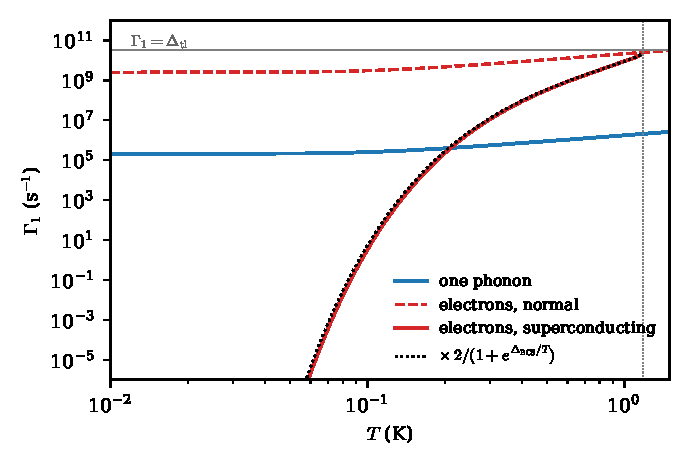
\includegraphics[width=0.7\linewidth]{figures/ch16/fig16_8.pdf}
  \caption{Relaxation rates of one two-level system in aluminum against temperature, for $\Delta_{\mathrm{tl}} = \SI{20.7}{\micro eV}$ (\SI{5}{GHz}) and $\Delta_0 = 0.3\,\Delta_{\mathrm{tl}}$. Blue: one phonon, \cref{eq:16.7-tau1}, with the model deformation potentials $\gamma_{\mathrm{l}} = \gamma_{\mathrm{t}} = \SI{1}{eV}$ and the isotropic sound speeds $c_{\mathrm{LA}} = \SI{6.63}{km.s^{-1}}$, $c_{\mathrm{TA}} = \SI{3.30}{km.s^{-1}}$ and density \SI{2.70}{g.cm^{-3}} of aluminum (\cref{sec:20.3}). Red dashed: conduction electrons in the normal state, \cref{eq:16.8-black}, with $\alpha_{\mathrm{ohm}} = 0.28$, continued below $T_c = \SI{1.18}{K}$ (vertical line) as for a film held normal. Red solid: the superconducting state, from the quasiparticle integral of \cref{app:D.42} with the weak-coupling gap $\Delta_{\mathrm{BCS}}(T)$; black dotted: the normal rate times $2/(1 + \ee^{\Delta_{\mathrm{BCS}}/T})$. The gray line marks $\varGamma_1 = \Delta_{\mathrm{tl}}$, which the normal-state rate reaches at \SI{1.5}{K}, where the golden rule fails.}
  \label{fig:16-tlsrates}
\end{figure}

\begin{limitbox}[Two-level relaxation by phonons and electrons][lim:16.8a]
The published rates are Jäckle's one-phonon rate and Black's electron rate, \cref{eq:16.7-tau1,eq:16.8-black}, with the superconducting factor $2/(1 + \ee^{\Delta_{\mathrm{BCS}}/T})$~\cite[Eqs.~(7)--(9)]{meissner2021acoustic}, and the Born-limit coupling $\alpha_{\mathrm{ohm}} = 4K_{\mathrm{b}}$~\cite[Eq.~(4)]{maillet2023nanomechanical}.
\par\smallskip
{\centering
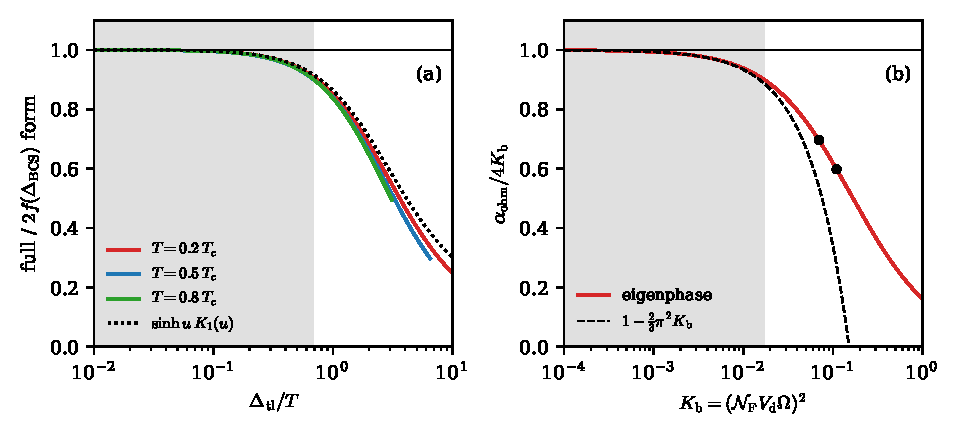
\includegraphics[width=\linewidth]{figures/ch16/limit16_8a.pdf}
\captionof{figure}{(a) Electron relaxation rate of a two-level system in superconducting aluminum, from the quasiparticle integral with the case-I coherence factor and the weak-coupling gap ($T_c = \SI{1.18}{K}$), divided by the normal rate times $2/(1 + \ee^{\Delta_{\mathrm{BCS}}/T})$, against $\Delta_{\mathrm{tl}}/T$ at $T = 0.2$, 0.5 and $0.8\,T_c$; each curve ends at $\Delta_{\mathrm{tl}} = 2\Delta_{\mathrm{BCS}}(T)$. Dotted: the closed form $\sinh u\,K_1(u)$, $u = \Delta_{\mathrm{tl}}/2T$, of \cref{eq:16.8-sc}. Gray: within \SI{10}{\percent} of one, $\Delta_{\mathrm{tl}} \le 0.69$--$0.73\,T$. (b) Ohmic coupling from the scattering phases of one contact channel per spin, $\alpha_{\mathrm{ohm}} = (4/\pi^2)\arctan^2(\pi K_{\mathrm{b}}^{1/2})$, divided by the Born value $4K_{\mathrm{b}}$, against $K_{\mathrm{b}}$. Dashed: the leading correction $1 - \tfrac23\pi^2K_{\mathrm{b}}$. Dots: the resonator fits $K_{\mathrm{b}} = 0.07$ and 0.11. Gray: within \SI{10}{\percent}, $K_{\mathrm{b}} \le 0.017$.}\label{fig:16-limit-tlsrel}
\par}
\smallskip
For $\Delta_{\mathrm{tl}} \gtrsim T$ the quasiparticles cannot take up the splitting as freely as normal electrons, and for $K_{\mathrm{b}} \gtrsim 0.02$ the phase shift of a single channel is no longer small, so that the Born coupling overstates $\alpha_{\mathrm{ohm}}$.
\end{limitbox}

\subsection{The ohmic scaling limit}\label{sec:16.8-ohmic}

The fitted couplings are not small, and \cref{fig:16-tlsrates} shows the consequence: the normal-state rate of \cref{eq:16.8-black} reaches the splitting itself at \SI{1.5}{K}, and for a symmetric defect, $\Delta_0 = \Delta_{\mathrm{tl}}$, it is at least $0.88\,\Delta_{\mathrm{tl}}$ at every temperature, since $\varGamma_1^{\mathrm{el}}/\Delta_{\mathrm{tl}} = \pi\alpha_{\mathrm{ohm}}\coth(\Delta_{\mathrm{tl}}/2T)$ with $\alpha_{\mathrm{ohm}} = 0.28$. A defect damped at a rate comparable to its splitting has no eigenstates to relax between. The electrons then dephase the two configurations faster than the defect tunnels, and the defect hops between $|\mathrm{L}\rangle$ and $|\mathrm{R}\rangle$ at the incoherent rate of \cref{eq:C.20-rate}, second order in $\Delta_0$ and exact in $\alpha_{\mathrm{ohm}}$. \Cref{app:C.20} evaluates it for the ohmic bath, \cref{eq:C.20-ohmrate}, and shows that for $\Delta_0, T \ll \omega_{\mathrm{cut}}$ the cutoff enters only through the renormalized tunneling amplitude $\Delta_{\mathrm{r}}$ of \cref{eq:C.20-Dr}. For a symmetric defect the relaxation rate $\varGamma_{\mathrm{LR}} + \varGamma_{\mathrm{RL}}$ is then
\begin{equation}
  \varGamma_{\mathrm{LR}} + \varGamma_{\mathrm{RL}} = \frac{\Gamma(1 + \alpha_{\mathrm{ohm}})}{\Gamma(1 - \alpha_{\mathrm{ohm}})}\,\frac{\Delta_{\mathrm{r}}^{2(1 - \alpha_{\mathrm{ohm}})}}{\alpha_{\mathrm{ohm}}}\,(2\pi T)^{2\alpha_{\mathrm{ohm}} - 1} ,
  \qquad \Delta_{\mathrm{r}} \ll T \ll \omega_{\mathrm{cut}} ,
  \label{eq:16.8-scaling}
\end{equation}
with $\Gamma(z)$ Euler's gamma function; the form follows from \cref{eq:C.20-ohmrate} at $\Delta_{\mathrm{as}} = 0$ with the duplication and reflection formulas of $\Gamma$. The rate depends on $\Delta_0$ and $\omega_{\mathrm{cut}}$ only through $\Delta_{\mathrm{r}}$, which is what makes it a scaling limit. It grows as the temperature falls whenever $\alpha_{\mathrm{ohm}} < \tfrac12$, the anti-Arrhenius law: at $\alpha_{\mathrm{ohm}} = 0.28$ it scales as $T^{-0.44}$, and as $\alpha_{\mathrm{ohm}} \to 0$ as $1/T$. A thermally activated rate would do the opposite. \Cref{app:C.20} traces the growth to the slower dephasing by the electrons at low temperature, over the time $1/T$, which wins against the shrinking dressed amplitude.

Qureshi obtained the same dynamics from the bosonized electron gas~\cite{qureshi1995dynamics}. Without electron-assisted tunneling his Laplace-transformed correlation function of $\sigma_z$~\cite[Eqs.~(8), (9)]{qureshi1995dynamics} is the noninteracting-blip result of \cref{app:C.20}, and his coupling $K$ is $\alpha_{\mathrm{ohm}}$ in the normalization of \cref{eq:C.20-ohmic}, not $K_{\mathrm{b}}$. For a symmetric defect and $\alpha_{\mathrm{ohm}} \ll 1$ he reduces it to~\cite[Eq.~(10)]{qureshi1995dynamics}
\begin{equation}
  \begin{gathered}
  \hat C(z) \simeq \frac{1}{z + \tilde\Delta_0^2/(z + \gamma_0)} , \qquad \gamma_0 = 2\pi\alpha_{\mathrm{ohm}}T , \\
  \tilde\Delta_0^2 = \Gamma(1 - 2\alpha_{\mathrm{ohm}})\cos(\pi\alpha_{\mathrm{ohm}})\,\Delta_0^2\Bigl(\frac{2\pi T}{\omega_{\mathrm{cut}}}\Bigr)^{2\alpha_{\mathrm{ohm}}} .
  \end{gathered}
  \label{eq:16.8-qureshi}
\end{equation}
Its poles describe both regimes of this section. For $\tilde\Delta_0 > \gamma_0/2$ the defect oscillates at a frequency near $\tilde\Delta_0$ and its $\sigma_z$ correlation decays at $\gamma_0/2 = \pi\alpha_{\mathrm{ohm}}T$. For a symmetric defect with $T \gg \Delta_{\mathrm{tl}}$ this is half of \cref{eq:16.8-black}, the decay of an off-diagonal quantity at $\varGamma_1/2$, so Black's rate is the weakly damped side of \cref{eq:16.8-qureshi}. For $\tilde\Delta_0 < \gamma_0/2$ the motion is overdamped and the slow pole gives the relaxation rate $\tilde\Delta_0^2/\gamma_0$. By \cref{eq:C.20-Dr}, $\tilde\Delta_0^2 = \Delta_{\mathrm{r}}^{2(1 - \alpha_{\mathrm{ohm}})}(2\pi T)^{2\alpha_{\mathrm{ohm}}}$, and $\tilde\Delta_0^2/\gamma_0$ is \cref{eq:16.8-scaling} without the factor $\Gamma(1 + \alpha_{\mathrm{ohm}})/\Gamma(1 - \alpha_{\mathrm{ohm}}) = 1 - 2\gamma_{\mathrm{E}}\alpha_{\mathrm{ohm}} + O(\alpha_{\mathrm{ohm}}^2)$, which is \SI{10}{\percent} below one at $\alpha_{\mathrm{ohm}} = 0.091$ and 0.71 at the fitted 0.28 (\cref{lim:16.8b}). The boundary $\tilde\Delta_0 = \gamma_0/2$ is a temperature,
\begin{equation}
  T_{\mathrm{coh}} = \frac{\Delta_{\mathrm{r}}}{2\pi}\Bigl(\frac{2}{\alpha_{\mathrm{ohm}}}\Bigr)^{1/(1 - \alpha_{\mathrm{ohm}})} ,
  \label{eq:16.8-Tcoh}
\end{equation}
below which a symmetric defect tunnels coherently, with weak damping, and above which it hops. For $\alpha_{\mathrm{ohm}} \ll 1$ it is $\Delta_{\mathrm{r}}/\pi\alpha_{\mathrm{ohm}}$, the temperature at which $\pi\alpha_{\mathrm{ohm}}T$ reaches the splitting; at $\alpha_{\mathrm{ohm}} = 0.28$ the small-coupling form of \cref{eq:16.8-qureshi} puts it at $2.4\,\Delta_{\mathrm{r}}$, where the scaling form \cref{eq:16.8-scaling} is itself at the edge of its range. An asymmetric defect, $\Delta_{\mathrm{as}} \gg \Delta_0$, is weakly damped as long as \cref{eq:16.8-black} stays below $\Delta_{\mathrm{tl}}$, and most defects of a glass are of this kind (\cref{sec:16.7}); the scaling limit concerns the nearly symmetric ones and light interstitials in metals.

\begin{limitbox}[The ohmic scaling limit][lim:16.8b]
The published relaxation rate of a symmetric tunneling defect in a metal is $\tilde\Delta_0^2/\gamma_0$, from the slow pole of \cref{eq:16.8-qureshi}, for $\alpha_{\mathrm{ohm}} \ll 1$~\cite[Eqs.~(8)--(10)]{qureshi1995dynamics}.
\par\smallskip
{\centering
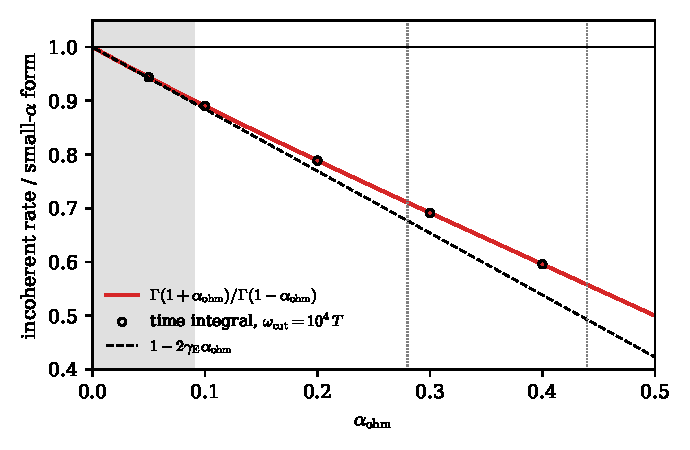
\includegraphics[width=0.75\linewidth]{figures/ch16/limit16_8b.pdf}
\captionof{figure}{Incoherent relaxation rate of a symmetric defect in an ohmic bath, \cref{eq:C.20-rate,eq:16.8-scaling}, divided by the small-coupling form $\tilde\Delta_0^2/\gamma_0$, against $\alpha_{\mathrm{ohm}}$. Red: the scaling limit $\Gamma(1 + \alpha_{\mathrm{ohm}})/\Gamma(1 - \alpha_{\mathrm{ohm}})$. Open circles: the time integral of \cref{eq:C.20-rate} done numerically with the full ohmic correlation exponent at $\omega_{\mathrm{cut}} = 10^4\,T$. Dashed: the leading correction $1 - 2\gamma_{\mathrm{E}}\alpha_{\mathrm{ohm}}$. Dotted lines: the Born values $\alpha_{\mathrm{ohm}} = 0.28$ and 0.44 of the aluminum resonator fits. Gray: within \SI{10}{\percent}, $\alpha_{\mathrm{ohm}} \le 0.091$.}\label{fig:16-limit-ohmic}
\par}
\smallskip
Outside the gray band the small-coupling form overstates the rate, by $1/0.71$ at $\alpha_{\mathrm{ohm}} = 0.28$, and both forms fail below $T \sim \Delta_{\mathrm{r}}$, where the defect tunnels coherently.
\end{limitbox}

\subsection{Thermally activated hopping and tunneling}\label{sec:16.8-hop}

A defect whose barrier $V_{\mathrm{b}}$ of \cref{sec:16.7} is large compared with $T$ can still cross it classically, at the rate $\varGamma = \varGamma_0\ee^{-V_{\mathrm{b}}/T}$ of harmonic transition-state theory (\cref{app:E.11}), with $\varGamma_0$ the attempt rate. In one dimension $\varGamma_0 = \omega_{\mathrm{w}}/2\pi$, with $\omega_{\mathrm{w}}$ the frequency of the well, and in many dimensions $\varGamma_0$ is Vineyard's ratio of the products of normal-mode frequencies at the minimum and at the saddle. This is the transition-state rate of Lawrence~\cite[Eq.~(1)]{lawrence2024semiclassical} with a classical, harmonic reactant partition function and transmission coefficient $\kappa = 1$. Tunneling through the top of the barrier raises the rate. For a barrier that is an inverted parabola of frequency $\omega^\ddagger$ the correction is exact,
\begin{equation}
  \kappa_{\mathrm{PB}} = \frac{\omega^\ddagger/2T}{\sin(\omega^\ddagger/2T)} = 1 + \frac{1}{24}\Bigl(\frac{\omega^\ddagger}{T}\Bigr)^2 + \frac{7}{5760}\Bigl(\frac{\omega^\ddagger}{T}\Bigr)^4 + \dots ,
  \label{eq:16.8-kappa}
\end{equation}
and its first two terms are Wigner's correction $\kappa_{\mathrm{W}}$~\cite[Eqs.~(2), (3)]{lawrence2024semiclassical}. The parabolic correction diverges at the crossover temperature
\begin{equation}
  T_\times = \frac{\omega^\ddagger}{2\pi} ,
  \label{eq:16.8-Tx}
\end{equation}
below which the particle no longer crosses near the top. It tunnels through the barrier at the energy that maximizes the product of the thermal weight and the transmission, along the instanton, the periodic path in imaginary time of period $1/T$, whose action $S_{\mathrm{inst}}$ replaces $V_{\mathrm{b}}/T$ in the exponent~\cite[Eq.~(4)]{lawrence2024semiclassical}. As $T \to 0$ the instanton becomes the tunneling path between the two minima, its action becomes twice the tunneling exponent $\lambda_{\mathrm{tun}}$ of \cref{sec:16.7}, and the hopping turns into the tunneling between $|\mathrm{L}\rangle$ and $|\mathrm{R}\rangle$ with amplitude $\Delta_0 \propto \ee^{-\lambda_{\mathrm{tun}}}$ that the previous sections assumed. For an atom with $\omega^\ddagger = \SI{10}{meV}$, $T_\times = \SI{18.5}{K}$, so at millikelvin temperatures every defect motion is tunneling, and a defect whose $\lambda_{\mathrm{tun}}$ is too large for it to tunnel within the time of an experiment is frozen. With an attempt rate of \SI{e13}{s^{-1}} and a year of observation, the bound is $\lambda_{\mathrm{tun}} \le 23.6$ when no energy-gap suppression adds to the exponent (\cref{app:E.22}).

\Cref{lim:16.8c} tests these forms on a barrier whose quantum rate is known exactly, the symmetric Eckart barrier $V(x) = V_{\mathrm{b}}\,\mathrm{sech}^2(x/L)$ with the hydrogen-atom parameters of Lawrence, $V_{\mathrm{b}} = 6\omega^\ddagger/\pi$. The exact rate exceeds the classical one by a factor 6.2 at $T_\times$ and 2.2 at $1.5\,T_\times$, so tunneling matters well above the crossover. Wigner's correction holds within \SI{10}{\percent} above $2.1\,T_\times$ and the parabolic form above $1.5\,T_\times$, while the instanton rate stays about \SI{18}{\percent} low between $0.25$ and $0.5\,T_\times$, an error that the higher terms of its asymptotic expansion in $\hbar$ would reduce~\cite[Sect.~III\,A]{lawrence2024semiclassical}.

Activation also fixes which defects of a glass contribute to its heat release. On cooling, defects with large barriers stay in equilibrium by activation until the activated rate falls below the rate at which the cooling changes $V_{\mathrm{b}}/T$, which is $V_{\mathrm{b}}|\dot T|/T^2$. Equating the two gives the freezing temperature
\begin{equation}
  T_{\mathrm{frz}} = \frac{V_{\mathrm{b}}}{\ln\bigl(\varGamma_0T_{\mathrm{frz}}^2/V_{\mathrm{b}}|\dot T|\bigr)} ,
  \label{eq:16.8-Tfrz}
\end{equation}
the form of Sahling et al.~\cite[Eq.~(8)]{sahling2010anomalous} with their $\tau_0 = 1/\varGamma_0$. Below $T_{\mathrm{frz}}$ the populations of these defects stop following the temperature, and the excess they keep is released later by tunneling.

\begin{limitbox}[Hopping and tunneling through one barrier][lim:16.8c]
The published rates are transition-state theory with Wigner's or the parabolic-barrier transmission, \cref{eq:16.8-kappa}, above the crossover temperature \cref{eq:16.8-Tx}, and the instanton rate below it~\cite[Eqs.~(1)--(4)]{lawrence2024semiclassical}.
\par\smallskip
{\centering
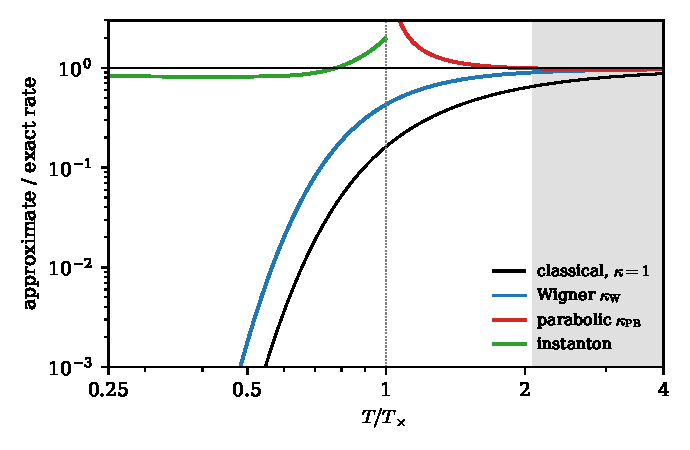
\includegraphics[width=0.75\linewidth]{figures/ch16/limit16_8c.pdf}
\captionof{figure}{Approximate thermal rates through a symmetric Eckart barrier divided by the exact quantum rate, against $T/T_\times$, for the hydrogen-atom parameters of Lawrence ($V_{\mathrm{b}} = \SI{248}{meV}$, $\omega^\ddagger = \SI{130}{meV}$, $T_\times = \SI{240}{K}$). Black: classical transition-state theory. Blue: with Wigner's correction. Red: with the parabolic-barrier correction, divergent at $T_\times$ (dotted line). Green: the instanton rate, for $T < T_\times$. The exact rate integrates the exact transmission probability of the Eckart barrier over the Boltzmann factor. Gray: Wigner's form within \SI{10}{\percent}, $T \ge 2.1\,T_\times$.}\label{fig:16-limit-hop}
\par}
\smallskip
Near $T_\times$ the expansion in $\omega^\ddagger/T$ diverges and the instanton is not yet formed, so neither form holds there, and below $T_\times$ the transition-state forms underestimate the rate by orders of magnitude.
\end{limitbox}

\subsection{Heat release of a cooled glass}\label{sec:16.8-heat}

A glass held at $T_{\mathrm{hi}}$ and cooled quickly to $T_{\mathrm{lo}}$ keeps its slow defects in the populations of $T_{\mathrm{hi}}$. A defect of splitting $\Delta_{\mathrm{tl}}$ has the mean energy $-\tfrac12\Delta_{\mathrm{tl}}\tanh(\Delta_{\mathrm{tl}}/2T)$ in equilibrium, so it holds the excess $\tfrac12\Delta_{\mathrm{tl}}[\tanh(\Delta_{\mathrm{tl}}/2T_{\mathrm{lo}}) - \tanh(\Delta_{\mathrm{tl}}/2T_{\mathrm{hi}})]$, which it gives to the phonons at its rate $\varGamma_1$ of \cref{eq:16.7-tau1}, evaluated at $T_{\mathrm{lo}}$. The defects are spread uniformly in the asymmetry $\Delta_{\mathrm{as}}$ and in the tunneling exponent $\lambda_{\mathrm{tun}}$, with density $\bar P$ (\cref{sec:16.7-stm})~\cite[Eq.~(1)]{sahling2010anomalous}. The slow defects have $\Delta_0 \ll \Delta_{\mathrm{as}}$, so $\Delta_{\mathrm{tl}} \simeq \Delta_{\mathrm{as}}$ is distributed uniformly too. Their excess energy, summed over $\Delta_{\mathrm{tl}}$, is
\begin{equation*}
  \int_0^\infty\dd\Delta_{\mathrm{tl}}\,\frac{\Delta_{\mathrm{tl}}}{2}\Bigl[\tanh\frac{\Delta_{\mathrm{tl}}}{2T_{\mathrm{lo}}} - \tanh\frac{\Delta_{\mathrm{tl}}}{2T_{\mathrm{hi}}}\Bigr] = \frac{\pi^2}{12}\bigl(T_{\mathrm{hi}}^2 - T_{\mathrm{lo}}^2\bigr) ,
\end{equation*}
since $1 - \tanh(x/2T) = 2/(\ee^{x/T} + 1)$ and $\int_0^\infty\dd x\,x/(\ee^{x/T} + 1) = \pi^2T^2/12$. The rate depends on the tunneling exponent through $\Delta_0^2 \propto \ee^{-2\lambda_{\mathrm{tun}}}$, so at fixed $\Delta_{\mathrm{tl}}$ a uniform density in $\lambda_{\mathrm{tun}}$ is a uniform density $\tfrac12$ per unit $\ln\varGamma_1$. A defect relaxes at time $t$ with probability $\varGamma_1\ee^{-\varGamma_1t}\dd t$, and summing over $\lambda_{\mathrm{tun}}$ gives $\int\dd\lambda_{\mathrm{tun}}\,\varGamma_1\ee^{-\varGamma_1t} = \tfrac12\int\dd\varGamma_1\,\ee^{-\varGamma_1t} = 1/2t$ whenever the rates extend far on both sides of $1/t$. The power released by a volume $\Vol$ of glass is therefore
\begin{keyresult}[Heat release of a cooled glass]
\begin{equation}
  \dot Q_{\mathrm{TLS}}(t) = \frac{\pi^2}{24}\,\bar P\,\Vol\,\frac{T_{\mathrm{hi}}^2 - T_{\mathrm{lo}}^2}{t} , \qquad \varGamma_{\max}^{-1} \ll t \ll \varGamma_{\min}^{-1} ,
  \label{eq:16.8-heat}
\end{equation}
\end{keyresult}
with $\varGamma_{\max}$ and $\varGamma_{\min}$ the fastest and slowest one-phonon rates at $T_{\mathrm{lo}}$ of the defects with $\Delta_{\mathrm{tl}} \sim T_{\mathrm{hi}}$, which hold most of the excess. This is the law of Sahling et al.~\cite[Eq.~(6)]{sahling2010anomalous}. The $1/t$ comes from the uniform density in $\lambda_{\mathrm{tun}}$, and the prefactor depends neither on the deformation potentials nor on the sound speeds, which only shift the window in time. Since every decade of time draws on defects in a range of $\lambda_{\mathrm{tun}}$ of width $\tfrac12\ln10$, the heat released between $t_1$ and $t_2$ is the prefactor times $\ln(t_2/t_1)$, and the heat measured at a time $t$ comes from defects with $\varGamma_1 \approx 1/t$. If the glass starts above $T_{\mathrm{frz}}$ of \cref{eq:16.8-Tfrz}, the defects that release at time $t$ were last in equilibrium at $T_{\mathrm{frz}}$, and $T_{\mathrm{frz}}$ replaces $T_{\mathrm{hi}}$~\cite[Eq.~(7)]{sahling2010anomalous}; the release then no longer grows with the starting temperature.

\begin{limitbox}[Heat release of a cooled glass][lim:16.8d]
The published heat release after a quench from $T_{\mathrm{hi}}$ to $T_{\mathrm{lo}}$ is \cref{eq:16.8-heat}~\cite[Eqs.~(1), (6)--(8)]{sahling2010anomalous}.
\par\smallskip
{\centering
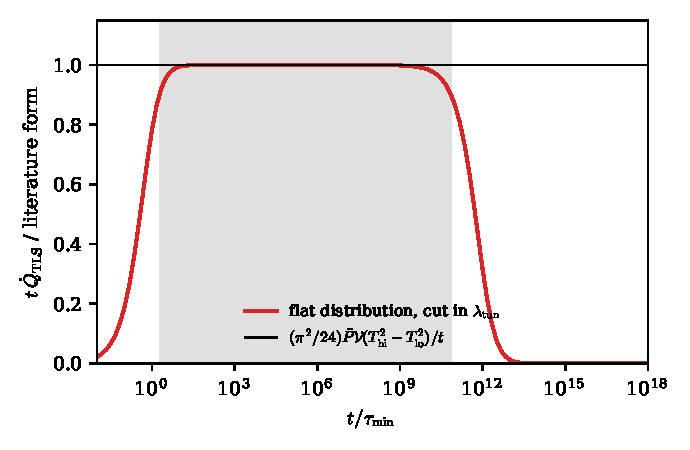
\includegraphics[width=0.75\linewidth]{figures/ch16/limit16_8d.pdf}
\captionof{figure}{Heat release of a model glass times $t$, divided by the prefactor of \cref{eq:16.8-heat}, against $t$ in units of $\tau_{\min}$, the relaxation time of the fastest defect at $\Delta_{\mathrm{tl}} = T_{\mathrm{hi}}$. Red: the uniform distribution cut at $\lambda_{\mathrm{min}} \le \lambda_{\mathrm{tun}} \le \lambda_{\mathrm{min}} + 14$, with the exact splitting $\Delta_{\mathrm{tl}} = (\Delta_{\mathrm{as}}^2 + \Delta_0^2)^{1/2}$, $\Delta_0 \le 0.1\,T_{\mathrm{lo}}$, the one-phonon rate \cref{eq:16.7-tau1} at $T_{\mathrm{lo}}$ and an instantaneous quench with $T_{\mathrm{lo}}/T_{\mathrm{hi}} = 1/480$ (\SI{10}{mK} after \SI{4.8}{K}). Gray: within \SI{10}{\percent} of one, $1.8\,\tau_{\min} \le t \le 7.1\times10^{10}\,\tau_{\min}$, 10.6 of the 12.2 decades that the cut spans.}\label{fig:16-limit-heat}
\par}
\smallskip
Outside the window the release falls below the $1/t$ law, at early times because the fastest defects have already relaxed and at late times because the distribution of tunneling exponents ends.
\end{limitbox}

Inside its window \cref{eq:16.8-heat} is exact for the uniform distribution: in \cref{lim:16.8d} it holds within $2\times10^{-4}$ from $10^2$ to $10^8\,\tau_{\min}$. The tests of the law are therefore tests of the distribution. Heat-release measurements on vitreous silica follow $1/t$ and $T_{\mathrm{hi}}^2 - T_{\mathrm{lo}}^2$, but they give a density $\bar P$ four times smaller than the specific heat measured over seconds, $2.0\times10^{44}$ against $8.0\times10^{44}\,\si{J^{-1}.m^{-3}}$~\cite[Table~1]{sahling2014anomalous}. Sahling et al.\ attribute the difference to defects whose barriers are lowered by local stresses frozen in on cooling. These relax within about \SI{100}{s}, before the heat-release measurement starts, and a small fraction of them, \SI{5}{\percent}, freezes at \SI{14.5}{K} instead of \SI{4.8}{K} and adds to the release after a quench from higher temperatures~\cite{sahling2014anomalous}. The specific-heat value, $1.28\times10^{20}\,\si{eV^{-1}.cm^{-3}}$, is close to the $1.2\times10^{20}\,\si{eV^{-1}.cm^{-3}}$ that the polarization-averaged acoustic tunneling strength implies for $\gamma_{\mathrm{l}} = \SI{1}{eV}$ ($0.88\times10^{20}$ with the longitudinal $C_{\mathrm{l}}$; \cref{sec:16.7}).

\begin{workedexample}{Heat release of one gram of fused silica at \SI{10}{mK}}\label{we:16-heat}
Take \SI{1}{g} of vitreous silica, $\Vol = \SI{0.455}{cm^3}$ at the density $\rho_T = \SI{2.2}{g.cm^{-3}}$ of \cref{sec:16.7}, cooled from room temperature to $T_{\mathrm{lo}} = \SI{10}{mK}$. The defects that release over hours to weeks freeze at $T_{\mathrm{frz}} = \SI{4.8}{K}$, and the heat-release density is $\bar P = 2.0\times10^{44}\,\si{J^{-1}.m^{-3}} = 3.20\times10^{19}\,\si{eV^{-1}.cm^{-3}}$~\cite[Table~1]{sahling2014anomalous}. With $T_{\mathrm{frz}}$ in place of $T_{\mathrm{hi}}$, and $T_{\mathrm{lo}}^2/T_{\mathrm{frz}}^2 = 4\times10^{-6}$ negligible, \cref{eq:16.8-heat} gives
\begin{equation*}
  \begin{split}
  t\,\dot Q_{\mathrm{TLS}} &= \frac{\pi^2}{24}\,k_{\mathrm{B}}^2\,\bar P\,\Vol\,T_{\mathrm{frz}}^2 \\
  &= 0.4112\times(\SI{1.381e-23}{J.K^{-1}})^2\times\SI{2.0e44}{J^{-1}.m^{-3}} \\
  &\qquad\times\SI{4.55e-7}{m^3}\times(\SI{4.8}{K})^2 \\
  &= \SI{1.64e-7}{J} .
  \end{split}
\end{equation*}
One hour after the cooling the sample releases $\SI{1.64e-7}{J}/\SI{3600}{s} = \SI{46}{pW}$, after a day \SI{1.9}{pW}, and after a week \SI{0.27}{pW}. Between the first hour and the end of the first week it gives off $\SI{1.64e-7}{J}\times\ln168 = \SI{0.84}{\micro J}$, or $5\times10^{12}\,\si{eV}$. With the specific-heat density the power would be four times larger. The fraction of defects that freezes at \SI{14.5}{K} is $0.05\times3 = 0.15$ of the normal density, with 3 the ratio of the stress-lowered defects to the normal density, $(8.0 - 2.0)/2.0$. By the square of its freezing temperature it adds another 1.4 times the normal release after a quench from above \SI{14.5}{K}, with the freezing temperatures of the table of Sahling et al. Their text quotes 5.5 and \SI{14.1}{K}, which give 0.99, and states that the anomalous part is roughly twice the normal one~\cite{sahling2014anomalous}. A hundred grams of fused silica near a detector at \SI{10}{mK} thus deposits \SI{4.6}{nW} an hour after cooling and \SI{0.19}{nW} a day later, a load and a source of delayed events that \cref{sec:19.6} takes up.
\end{workedexample}

\subsection{Interacting two-level systems}\label{sec:16.8-open}

Every result of this section treats the defects as independent, yet two defects interact through the strain fields each creates, with a coupling that falls as $1/r^3$. Its typical size relative to the spread of their splittings is the tunneling strength $C = \bar P\gamma_{\mathrm{l}}^2/\rho_Tc_{\mathrm{LA}}^2$, $2.6\times10^{-4}$ in vitreous silica (\cref{sec:16.7}). Thermal flips of neighbors shift the splitting of a given defect in time, which is spectral diffusion; it broadens single lines, and qubit spectroscopy sees it directly~\cite[Sect.~IV]{muller2019towards}. An ensemble whose spectrum is flat in $\Delta_{\mathrm{tl}}$ is unchanged by a normalized shift kernel away from the edges of the band. Spectral diffusion alone therefore leaves the ensemble responses of \cref{sec:16.7} intact, but it changes which defects relax at a given time and so the window of \cref{eq:16.8-heat}. The phonon emitted by one relaxing defect can trigger the relaxation of another. If each release triggers on average $b_{\mathrm{br}}$ more, a branching process, the mean size of a cascade of releases is $1/(1 - b_{\mathrm{br}})$, finite for $b_{\mathrm{br}} < 1$, and the distribution of the cascade size $N_{\mathrm{casc}}$ approaches $N_{\mathrm{casc}}^{-3/2}$ as $b_{\mathrm{br}} \to 1$. Such avalanches would turn the steady $1/t$ release into bursts. None of this is quantified for a real glass: $b_{\mathrm{br}}$ needs the density of barriers below the energy of the emitted phonons and the flux of ballistic phonons through the triggering volume, and no calculation or measurement of it exists. Whether the delayed events of a cooled detector are independent relaxations or avalanches of this kind is the open question that \cref{sec:19.6} inherits.

\section{Material inputs of the novel targets}\label{sec:16.9}

Two first-principles calculations of the dielectric tensor of ZrTe$_5$ give 20.75 and 9.8 along its slow axis, and the scattering reach of the material moves by a factor 2.8 between them (\cref{we:16-band}). Both numbers enter \cref{eq:16.1-L} exactly; no approximation of the response is involved, and a measurement of the tensor would settle the question. Most targets of this chapter are limited in the same way. The loss tangent of amorphous SiO$_2$ changes seventeenfold between preparations. And the probability that a single nuclear recoil of a few hundred eV in LiF leaves a readable F center has not been measured. \Cref{tab:16-inputs} lists, for each target, the inputs its rate needs, how well they are known and how their uncertainty moves the reach.

\subsection{Measured, computed and unmeasured inputs}\label{sec:16.9-inputs}

Some inputs of \cref{tab:16-inputs} are measured constants that vary from sample to sample: the loss tangent of a glass, the width of a donor line, the work function of a sheet on its substrate, the Luttinger parameter of a nanotube. The spread between samples is then the uncertainty of the input, and a detector that characterizes its own crystal or film removes it.

Others are computed constants, such as the dielectric tensor and the half-gap of a Dirac material, the Bloch-overlap coefficients $\mathcal{U}_{j'j}(\vect{G})$ of a donor, or the ohmic coupling $\alpha_{\mathrm{ohm}}$ of a tunneling defect. Their uncertainty is the spread between calculations, or the spread of a calculation over its functional and numerical choices. Such a spread is an estimate, not a bound: two calculations need not bracket the true value.

A third group are yields and parameters that no measurement isolates. One is the four factors of \cref{eq:16.6-yield} for single recoils of tens to hundreds of eV at millikelvin temperatures (\cref{sec:16.6-yields}); another is the density, dipole moment and deformation potential of two-level systems one by one (\cref{sec:16.7-open}), on which the estimate of \cref{sec:16.7-scat} rests through an assumed deformation potential of \SI{1}{eV}. For these inputs \cref{sec:8.8} assigns no width, and a reach is conditional on the value assumed.

\begin{table}[tbp]
  \caption{Material inputs of the novel targets, with their values, their uncertainty and its effect on the reach. The truncations of the responses are in \cref{tab:16-nuisances}.}
  \label{tab:16-inputs}
  \centering\scriptsize\setlength{\tabcolsep}{3pt}
  \begin{tabular}{@{}>{\raggedright\arraybackslash}p{0.15\linewidth}>{\raggedright\arraybackslash}p{0.38\linewidth}>{\raggedright\arraybackslash}p{0.43\linewidth}@{}}
    \toprule
    Target & Inputs (values) & Uncertainty and effect on the reach \\
    \midrule
    Dirac material (ZrTe$_5$) & background tensor $\varepsilon_{\mathrm{bg},ii} = 308.4$, 20.75, 126.1 (computed; earlier 187.5, 9.8, 90.9); velocities, cutoff \SI{0.191}{eV} and half-gap $\Delta_{\mathrm{D}} = \SI{11.8}{meV}$ of the measured-structure row (computed half-gaps 11.8--\SI{17.5}{meV}; measured \SI{11.75}{meV}) & between the two tensors $\sigmae^{\mathrm{lim}}$ moves by 2.8 to 2.9 and $\zeta^{\mathrm{lim}}$ by 1.8 to 2.0 (\cref{we:16-band}); the Dirac term inside the computed tensor, 3 to \SI{8}{\percent}, moves $\sigmae^{\mathrm{lim}}$ by 0.88; the computed half-gaps move the threshold mass along the slow axis from 7.1 to \SI{10.6}{keV} \\
    Metallic nanotubes, doped graphene & $g_c$ (measured 0.2--0.7; 0.17--0.34 for $r_{\mathrm{t}} = \SI{0.7}{nm}$ in vacuum); Fermi energy; substrate & line weight $\propto N_{\mathrm{ch}}g_c$; Fermi energy and substrate set the sheet plasmon \\
    Vacuum ejection (graphene) & work function $\Phi_{\mathrm{wf}} \simeq \SI{4.3}{eV}$ (substrate-dependent); occupied orbitals and binding energies & threshold mass $2\Phi_{\mathrm{wf}}/v_{\mathrm{max}}^2 = \SI{1.22}{MeV}$ moves with $\Phi_{\mathrm{wf}}$ \\
    Quantum dots (PbS in silica) & dot gap \SI{1.2}{eV} at \SI{3.3}{nm}; $\varepsilon_{\mathrm{in}}(\omega)$ of the dots; host $\varepsilon_{\mathrm{out}}$ & depolarization factor 0.57 to 6.7 for the cases of \cref{we:16-depol}, $\zeta^{\mathrm{lim}}$ moved by 1.33 to 0.39, sign unknown over 2.5--\SI{10}{eV} \\
    Molecular crystals (anthracene) & lowest singlet \SI{3.1}{eV} and crystal structure (measured); form factors and Frenkel coupling $\mathfrak{J}$ ($\pi$-electron model); transfer integral $t_{\mathrm{CT}}$ & model corrections in \cref{tab:16-nuisances} \\
    Dopants (Si:P) & level energies (measured); line strengths (central-cell model); line width $\ge \SI{4.22}{\micro eV}$; donor density against $\nd_{\mathrm{c}} \approx \SI{3e18}{cm^{-3}}$; local-field ratio $\mathfrak{f}^{\mathrm{loc}}_{\mathrm{D}}$ & resonant rate $\propto \nd_{\mathrm{D}}/\varGamma_{\mathrm{line}}$, $\zeta^{\mathrm{lim}} = \num{2.3e-16}$ at the $2p_0$ line for \SI{e15}{cm^{-3}}; $\mathfrak{f}^{\mathrm{loc}}_{\mathrm{D}}$ close to one, unsized \\
    Color centers (LiF) & displacement threshold $E_{\mathrm{d}} = \SI{27}{eV}$ (simulation input); site phonon energy 33.5--\SI{77.2}{meV}; yields $p_{\mathrm{FP}}$, $p_{\mathrm{surv}}$, $p_q$, $f_{\mathrm{opt}}$, $p_{\mathrm{FH}}$ & lightest mass 0.113--\SI{0.255}{GeV} for $E_{\mathrm{d}} = 10$--\SI{50}{eV}; yields unmeasured, the reach scales as $1/Y_{\mathrm{CC}}$ \\
    Bond breaking (H$_2$, molecular crystals) & bond energy \SI{4.75}{eV} and $\omega_{\mathrm{vib}} = \SI{0.546}{eV}$ (measured); cage escape $p_{\mathrm{esc}}$; yields of repulsive electronic states & $p_{\mathrm{esc}}$ and electronic yields unmeasured \\
    Glasses (a-SiO$_2$) & $\tan\delta_0$; $\varepsilon_r = 3.9$ (assumed); acoustic tunneling strength $C_{\mathrm{l}}$ (measured); $\bar P$, $\gamma_{\mathrm{l}}$ ($\SI{1}{eV}$ assumed), dipole moment & $\tan\delta_0 = 3\times10^{-4}$ (thermal oxide) to $5\times10^{-3}$ (deposited oxide): absorption rate $\times16.7$, $\zeta^{\mathrm{lim}}$ $\times4.1$; scattering host term fixed by $C_{\mathrm{l}}$ alone, core term needs $\bar P$ and $\gamma_{\mathrm{l}}$ \\
    Two-level systems at millikelvin & $\alpha_{\mathrm{ohm}} = 4K_{\mathrm{b}}$ (Born), $K_{\mathrm{b}} = 0.07$, 0.11 fitted (aluminum); $\bar P$ of vitreous silica $2.0\times10^{44}$ (heat release) or $8.0\times10^{44}\,\si{J^{-1}.m^{-3}}$ (specific heat) & heat release fourfold between the two $\bar P$; first-principles $\alpha_{\mathrm{ohm}}$ needs the scattering phases of both configurations \\
    \bottomrule
  \end{tabular}
\end{table}

\subsection{Theory-limited and data-limited targets}\label{sec:16.9-limits}

A target is limited by theory when its response has no controlled approximation at the values its inputs take, so that better inputs would not sharpen the rate. Dirac cones at strong coupling (\cref{sec:16.1-validity}), donors near the Mott density (\cref{sec:16.5-band}) and interacting two-level systems (\cref{sec:16.8-open}) are of this kind.

A second group is limited by a calculation whose formalism is known. The electron--hole ladder near the edge of a Dirac material changes the rate of ZrTe$_5$ by the Sommerfeld factor, 1.5 or more, at \SI{20}{keV} and by less above \SI{100}{keV} (\cref{sec:16.1-validity}). So do the final state of an ejected electron, the periodic Bethe--Salpeter response of a molecular crystal at finite $\vect{q}$, the excitons of a semiconducting tube and the valley-orbit coefficients of a donor. The response of a layered stack beyond its effective medium and the ohmic coupling $\alpha_{\mathrm{ohm}}$ from first principles complete the group. In each case the next term has a definite form and is computable, but no computation of it exists for the material.

The remaining targets are limited by data. Their inputs are properties of the sample that a measurement fixes: the dielectric tensor and the gap of ZrTe$_5$, the dielectric function $\varepsilon_{\mathrm{in}}(\omega)$ of real quantum dots, the oscillator strengths of the donor lines, the displacement threshold of LiF as a function of direction, the four yields of a color center, and the parameters of the two-level systems of a given film; \cref{sec:16.6-yields} names the measurements of the yields. For these inputs the response formula is in hand, and the uncertainty of the rate is that of the sample.

\subsection{Reach bands from input uncertainties}\label{sec:16.9-band}

An input $x$ on which the rate depends as a power, $\mathcal{R} \propto x^{-p}$ over the energies the rate samples, is a normalization uncertainty in the sense of \cref{sec:8.8}. By \cref{eq:1.5-limscaling} it moves a scattering reach as $\sigmae^{\mathrm{lim}} \propto x^{p}$, so a range $x_1 < x < x_2$ becomes a band of constant width $(x_2/x_1)^p$ in $\sigmae^{\mathrm{lim}}$ wherever $p$ does not change with the mass. An absorption reach moves as $\mathcal{R}^{-1/2}$, and its band is half as wide on a logarithmic scale. An input that sets a threshold acts instead through the low-mass wall, $\delta\ln m_{\mathrm{min}} = \delta\ln E_{\mathrm{th}}$ by \cref{eq:1.3-mmin}, and near the wall its band widens without limit (\cref{eq:8.8-shift}). An input without a size, such as the yield of a color center, gives no band: the reach is drawn for an assumed value and moves as its inverse.

For a Dirac material the power follows from \cref{eq:16.1-L}. At fixed Dirac parameters,
\begin{equation}
  \frac{\partial\ln L}{\partial\ln\varepsilon_{\mathrm{bg}}} = -\frac{2\,\varepsilon_{\mathrm{bg}}\Real(\varepsilon_{\mathrm{bg}} + \varepsilon_{\mathrm{D}})}{|\varepsilon_{\mathrm{bg}} + \varepsilon_{\mathrm{D}}|^2} = -2\Bigl[1 - \frac{\Real\varepsilon_{\mathrm{D}}}{\varepsilon_{\mathrm{bg}}} + O\Bigl(\frac{|\varepsilon_{\mathrm{D}}|^2}{\varepsilon_{\mathrm{bg}}^2}\Bigr)\Bigr] ,
  \label{eq:16.9-power}
\end{equation}
since $\varepsilon_{\mathrm{bg}}$ is real and $\varepsilon_{\mathrm{D}}$ does not depend on it. The reach therefore moves almost as $\varepsilon_{\mathrm{bg}}^2$, less by twice the fraction of the screening that the Dirac electrons supply. For ZrTe$_5$ that fraction is 3 to \SI{8}{\percent} at long wavelength (\cref{we:16-band}).

\begin{workedexample}{The reach band of ZrTe$_5$ from its background tensor}\label{we:16-band}
Take the Dirac parameters of \cref{sec:16.1-zrte5}, the measured-structure row with $\Delta_{\mathrm{D}} = \SI{11.8}{meV}$, and the scattering reach of \cref{fig:16-zrte5}a: light mediator, orientation-averaged loss function, three events in a kg-year. The central tensor is $\varepsilon_{\mathrm{bg},ii} = 308.4$, 20.75 and 126.1~\cite[Table~2]{geilhufe2020dirac}. The earlier calculation of \cref{we:7-zrte5} gives 187.5, 9.8 and 90.9~\cite[Table~1]{hochberg2018detection}, smaller by factors of 0.61, 0.47 and 0.72. We combine it with the same velocities, gap and cutoff, which isolates the effect of the tensor; the two calculations also differ in their velocities.

\emph{Estimate.} At weak screening $L \to \Imag\varepsilon_{\mathrm{D}}/(\hat{\vect{q}}\cdot\varepsilon_{\mathrm{bg}}\cdot\hat{\vect{q}})^2$. If $\Imag\varepsilon_{\mathrm{D}}$ were the same in every direction, the reach would move by the ratio of the direction averages of $(\hat{\vect{q}}\cdot\varepsilon_{\mathrm{bg}}\cdot\hat{\vect{q}})^{-2}$, which is 0.327 for the earlier tensor against the central one. Directions within \ang{30} of the slow axis $y$, where the background is smallest, carry \SI{64}{\percent} of that average for the central tensor, so the band is set mainly by $\varepsilon_{\mathrm{bg},yy}$, $(9.8/20.75)^2 = 0.22$ along the axis itself.

\emph{Full calculation.} With \cref{eq:16.1-L} and the anisotropic $\varepsilon_{\mathrm{D}}$ of \cref{eq:D.41-aniso}, the earlier tensor gives a reach 0.344 to 0.362 times the central one between \SI{20}{keV} and \SI{1}{MeV}, and 0.31 just above threshold. At the best mass, \SI{36}{keV}, the reach lies between $\SI{1.53e-40}{cm^2}$ and $\SI{5.5e-41}{cm^2}$, a band of 2.8 that is nearly constant in mass. The full ratio lies above the estimate because the smaller tensor lets the Dirac electrons screen more: the effective coupling along $y$ rises from 0.144 to 0.305.

\emph{Power.} Scaling the whole central tensor by 1.1 moves the reach by $1.1^p$ with $p = 1.86$ to 1.94 between \SI{20}{keV} and \SI{1}{MeV}, and $p = 1.85$ at \SI{12}{keV}, as \cref{eq:16.9-power} predicts for $\Real\varepsilon_{\mathrm{D}}/\varepsilon_{\mathrm{bg}}$ of a few percent. A tensor uncertain by a common factor of two would give a band of 3.6 to 3.8.

\emph{Dirac content.} Removing the static Dirac term of \cref{eq:7.3-aniso}, 10.0, 1.67 and 8.3 for this row, 3 to \SI{8}{\percent} of the components, leaves the background 298.4, 19.08 and 117.8, and moves the reach by 0.881 to 0.885, a correction smaller than the band.

\emph{Absorption.} For dark-photon absorption the earlier tensor moves $\zeta^{\mathrm{lim}}$ by 0.49 to 0.55 between the gap and the cutoff, from $1.24\times10^{-15}$ to $6.4\times10^{-16}$ at \SI{100}{meV}. The polarization along $y$ carries most of the rate, and for it alone $\zeta^{\mathrm{lim}} \propto \varepsilon_{\mathrm{bg},yy}$ at weak screening, which would give 0.47.

\emph{Gap.} The computed half-gaps of 11.8 to \SI{17.5}{meV} put the threshold mass along $y$ between 7.1 and \SI{10.6}{keV}, with \SI{9.4}{keV} for the relaxed-cell row at \SI{15.6}{meV}; the measured \SI{11.75}{meV} gives \SI{7.1}{keV}. Close to the wall the threshold band exceeds the tensor band, since it diverges there.
\end{workedexample}

Above \SI{100}{keV}, where the region near the pair edge carries less than a fifth of the rate, the tensor band is the largest sized uncertainty of the ZrTe$_5$ reach.

\section*{Summary}

A Dirac material screens the field of the dark matter with its whole dielectric function, $\varepsilon = \varepsilon_{\mathrm{bg}} + \varepsilon_{\mathrm{D}}$ (\cref{sec:16.1}). The published rates screen the Dirac electrons among themselves but not the field of the dark photon, and overstate scattering by $\varepsilon_{\mathrm{bg}}^2$ and absorption by $\varepsilon_{\mathrm{bg}}$ at every mass. For ZrTe$_5$ with the parameters of its measured structure the reach lies near \SI{1.5e-40}{cm^2} at \SI{40}{keV}, 5200 to 6400 times weaker than with the published rule for the standard halo.

Electrons confined to tubes and sheets respond to the momentum along them only, so a halo particle reaches a mode faster than $v_{\mathrm{max}}$ through an oblique momentum transfer, suppressed by the transverse form factor (\cref{sec:16.2}). An electron of graphene that receives more than the work function leaves the sheet with the direction of the momentum transfer, from \SI{1.22}{MeV} upward (\cref{sec:16.3}). The excitons of a molecular crystal follow from the Bethe--Salpeter equation in a molecular basis, and integrated over a window that holds whole manifolds, the crystal responds as a set of independent molecules at every momentum transfer, the Davydov sum rule (\cref{sec:16.4}).

Dilute donors in silicon add a response to first order in their density (\cref{sec:16.5}). The $2p_0$ line of Si:P at \SI{34.11}{meV} reaches $\zeta = \num{2.3e-16}$ at \SI{e15}{cm^{-3}}, twenty times below the continuum, and the first-order form fails at the line center from \SI{4.8e15}{cm^{-3}}. A color center forms after the prompt window: its rate is the recoil rate times the yield $Y_{\mathrm{CC}} = p_{\mathrm{FP}}p_{\mathrm{surv}}p_qf_{\mathrm{opt}}$ (\cref{sec:16.6}). A fluorine recoil in LiF above the simulation threshold of \SI{27}{eV} needs $\mchi \ge \SI{0.186}{GeV}$, and near threshold a recoil makes one vacancy and less than one free electron. Four yields at millikelvin temperatures are open, and each can be measured directly.

Glasses add tunneling two-level systems to the final states (\cref{sec:16.7}). A dark photon is absorbed at a rate proportional to $\zeta^2\tan\delta_0\tanh(m_\phi/2T)/\varepsilon_r$, the dielectric loss of the glass read at the dark-photon mass; on thermal SiO$_2$, three events in a kg-year at \SI{6}{GHz} need $\zeta = \num{2.44e-15}$. Coherent scattering off a random medium leaves the Born approximation once the optical potential exceeds about a tenth of the normal kinetic energy. Two-level systems whose populations froze near \SI{4.8}{K} release heat over hours to weeks after cooling (\cref{sec:16.8}). The density $\bar P$ inferred from heat release in vitreous silica is four times smaller than the one from its specific heat, and the fits to aluminum-coated resonators give $\alpha_{\mathrm{ohm}} = 0.28$ and 0.44, where the small-coupling rate fails. Whether the delayed events of a cooled detector are independent relaxations or avalanches of triggered releases is open, and \cref{sec:19.6} inherits the question.

The uncertainty budget of the chapter is \cref{tab:16-nuisances}, and \cref{tab:16-inputs} lists the material inputs, most of which only a measurement of the sample fixes (\cref{sec:16.9}).

\printbibliography[heading=subbibliography]
